%-----------------------------------------------------------------------
% Beginning of mcom-l-template.tex
%-----------------------------------------------------------------------
%
%     This is a topmatter template file for MCOM for use with AMS-LaTeX.
%
%     Templates for various common text, math and figure elements are
%     given following the \end{document} line.
%
%%%%%%%%%%%%%%%%%%%%%%%%%%%%%%%%%%%%%%%%%%%%%%%%%%%%%%%%%%%%%%%%%%%%%%%%

%     Remove any commented or uncommented macros you do not use.

\documentclass{mcom-l}

%     If you need symbols beyond the basic set, uncomment this command.
\usepackage{amssymb}

\usepackage[utf8]{inputenc}
\usepackage{bbm}
\usepackage[bbgreekl]{mathbbol}
% \usepackage{graphicx}
% \usepackage{graphicx,subfig}
\usepackage{graphicx,subfig,tikz} % include figures, create subfigures with \subfloat, draw with tikz
% \usepackage{MnSymbol}
\usepackage{comment}
% \usepackage{showkeys}

%     If the article includes commutative diagrams, ...
%\usepackage[cmtip,all]{xy}
\usepackage{tikz}
\usepackage{tikz-cd}
\usetikzlibrary{arrows,matrix}


%     Update the information and uncomment if AMS is not the copyright
%     holder.
%\copyrightinfo{2009}{American Mathematical Society}

\newtheorem{theorem}{Theorem}[section]
\newtheorem{corollary}[theorem]{Corollary}
\newtheorem{lemma}[theorem]{Lemma}

\theoremstyle{definition}
\newtheorem{definition}[theorem]{Definition}
\newtheorem{example}[theorem]{Example}
\newtheorem{xca}[theorem]{Exercise}
\newtheorem{assumption}[theorem]{Assumption}

\theoremstyle{remark}
\newtheorem{remark}[theorem]{Remark}

\numberwithin{equation}{section}

\newcommand{\csubfloat}[2][]{%
  \makebox[0pt]{\subfloat[#1]{#2}}%
}
\newcommand{\centerhfill}[1][\quad]{\hspace{\stretch{0.5}}#1\hspace{\stretch{0.5}}}

\definecolor{purple}{rgb}{1, 0, 1}

\newcommand{\ie}{\emph{i.e.,}\xspace}
\newcommand{\eg}{\emph{e.g.,}\xspace}
\newcommand{\abr}{\emph{abbr.}\xspace}
\newcommand{\ea}{\emph{et al.}\xspace}
\newcommand{\gensync}{\emph{GenSync}\xspace}
\newcommand{\colosseum}{\emph{Colosseum}\xspace}
\newcommand{\srep}{\emph{SREP}\xspace} % Set Reconciliation Enhances
\newcommand{\srepsim}{\emph{SREPSim}\xspace}
% Propagation
\newcommand{\esrep}{\emph{E-SREP}\xspace}
\newcommand{\epsrep}{\emph{EP-SREP}\xspace}
\newcommand{\mesrep}{\emph{ME-SREP}\xspace}
\newcommand{\mempoolsync}{\emph{MempoolSync}}

\newcommand{\fref}[1]{Fig.~\ref{#1}}
\newcommand{\tref}[1]{Table~\ref{#1}}
\newcommand{\aref}[1]{Algorithm~\ref{#1}}
\newcommand{\procref}[1]{Procedure~\ref{#1}}
\newcommand{\sref}[1]{Section~\ref{#1}}
\newcommand{\lineref}[1]{line~\ref{#1}}
\newcommand{\appref}[1]{Appendix~\ref{#1}}

% Change \eqref
\LetLtxMacro{\originaleqref}{\eqref}
\renewcommand{\eqref}{Eq.~\originaleqref}

% Theorems and corollaries
\newcounter{theoremcount}
\setcounter{theoremcount}{0}
\DeclareRobustCommand{\theorem}[1]{%
  \refstepcounter{theoremcount}%
  \noindent\textit{\textbf{Theorem \thetheoremcount\label{theorem:#1}: }}%
}
\DeclareRobustCommand{\theoremref}[1]{Theorem~\ref{theorem:#1}}

\DeclareRobustCommand{\proof}{\emph{Proof:}\xspace}
\DeclareRobustCommand{\qqed}{\hfill$\blacksquare$}

\newcounter{corollcount}
\setcounter{corollcount}{0}
\DeclareRobustCommand{\coroll}[1]{%
  \refstepcounter{corollcount}%
  \noindent\textit{\textbf{Corollary \thecorollcount\label{coroll:#1}: }}%
}
\DeclareRobustCommand{\corollref}[1]{Corollary~\ref{coroll:#1}}

\newcounter{lemmacount}
\setcounter{lemmacount}{0}
\DeclareRobustCommand{\lemma}[1]{%
  \refstepcounter{lemmacount}%
  \noindent\textit{\textbf{Lemma \thelemmacount\label{lemma:#1}: }}%
}
\DeclareRobustCommand{\lemmaref}[1]{Lemma~\ref{lemma:#1}}

\newcounter{definitioncount}
\setcounter{definitioncount}{0}
\DeclareRobustCommand{\definition}[1]{%
  \refstepcounter{definitioncount}%
  \noindent\textit{\textbf{Definition \thedefinitioncount\label{definition:#1}: }}%
}
\DeclareRobustCommand{\defref}[1]{Definition~\ref{definition:#1}}

%notes of different authors
\newif\ifnotes
\notestrue
\notesfalse

\newif\ifdiff
\difftrue
\difffalse

\newcommand{\anote}[1]{\ifnotes $\ll$\textsf{\textcolor{purple}{Ari: {#1}}}$\gg$ \fi}
\newcommand{\nnote}[1]{\ifnotes $\ll$\textsf{\textcolor{orange}{Novak: {#1}}}$\gg$ \fi}
\newcommand{\diff}[1]{\ifdiff\textcolor{orange}{#1}\else#1\fi}

%%% Local Variables:
%%% mode: latex
%%% TeX-master: "main"
%%% End:



% Hyperlinks in the document. According to the documentation:
%  "Make sure it comes last of your loaded packages, to give it
%   a fighting chance of not being over-written, since its job
%   is to redefine many LATEX commands"
\usepackage{hyperref}

\begin{document}

% \title[short text for running head]{full title}
\title[Bounded commuting projections for non-matching interfaces]%
	{Bounded commuting projections for multipatch spaces with non-matching interfaces}
% Stable commuting projections for multipatch spaces with local refinements

%    Only \author and \address are required; other information is
%    optional.  Remove any unused author tags.

%    author one information
% \author[short version for running head]{name for top of paper}
\author{Martin Campos Pinto}
\address{Max-Planck-Institut für Plasmaphysik, Boltzmannstr. 2, 85748 Garching, Germany}
% \curraddr{}
\email{martin.campos-pinto@ipp.mpg.de}
% \thanks{}

%    author two information
\author{Frederik Schnack}
\address{Max-Planck-Institut für Plasmaphysik, Boltzmannstr. 2, 85748 Garching, Germany}
% \curraddr{}
\email{frederik.schnack@ipp.mpg.de}
% \thanks{}

%    \subjclass is required.
\subjclass[2020]{%
% 65N30, %Finite element, Rayleigh-Ritz and Galerkin methods for boundary value problems involving PDEs
% 58A14, % Hodge theory in global analysis 
% 65N25, %Numerical methods for eigenvalue problems for boundary value problems involving PDEs
% 65N12% Stability and convergence of numerical methods for boundary value problems involving PDEs
}

\date{}

\dedicatory{}

%    Abstract is required.
\begin{abstract}
	We present stable commuting projection operators on de Rham sequences of 
	two-dimensional multipatch spaces with local tensor-product para{\-}metrization and 
	non-matching interfaces. 
	Our construction covers the case of shape-regular patches
	with different mappings and locally refined patches,
	under the assumption that neighboring patches have nested resolutions and that 
	interior vertices are shared by exactly four patches.
	Following a broken-FEEC approach we first apply a tensor-product construction on the single-patch de Rham sequences and modify the resulting patch-wise commuting projections to enforce their conformity while preserving their commuting, projection, and $L^2$ stability properties. The resulting operators are local and stable in $L^2$, 
	with constants independent of both the size and the inner 
	resolution of the individual patches.
	% Our commuting projection operators are also local, % in the sense of overlapping basis functions,
	% and their $L^2$ stability holds with constants independent 
	% The results are based on shape-regular patches that involve locally stable bases on , which are assumed to be nested across an interface and interior vertices are shared by exactly four patches.
	 % Our main finding is that this constructive process indeed produces local commuting projection operators on conforming spaces with uniform $L^2$ stability properties. 
\end{abstract}

\maketitle


\tableofcontents


\section{Introduction}


Mixed finite element spaces which preserve the de Rham structure 
offer a flexible and powerful framework for the approximation of partial
differential equations.
This discretization paradigm has been extensively studied in the scope of 
electromagnetic modelling
\cite{Bossavit.1988.IEE-A, Bossavit.1998.ap, Hiptmair.2002.anum}
and has given rise to an elegant body of theoretical work which guarantees that 
compatible spaces of nodal, egde, face and volume type
% approximating the $H^1(\Omega)$, $H(\curl;\Omega)$, $H(\Div;\Omega)$ 
% and $L^2(\Omega)$, 
lead to stable and accurate approximations to various 
differential operators %electromagnetic problems 
in domains with non-smooth or non-connected boundaries
\cite{Hiptmair.1999.mcomp, Compatible.2006.IMA, Boffi.2010.anum, boffi2011discrete}. 
% $\partial \Omega$.
% In particular the corresponding schemes do compute convergent solutions to Maxwell 
% or magnetostatic equations in the presence of reentrant corners (despite the fact 
% that singular fields $\bE \notin H^1(\Omega)$ may exist in the neighboorhood of 
% such corners), and they provide faithfully representations 
% of harmonic fields associated with tunnels or cavities in the computational domain.

A notable step has been the unifying analysis of Finite Element Exterior Calculus (FEEC)
\cite{Arnold.Falk.Winther.2006.anum, Arnold.Falk.Winther.2010.bams}
developped in the general framework of Hilbert complexes.
 % with further applications in solid mechanics ???
There, the existence of bounded cochain projections, i.e.~sequences of commuting projection operators with uniform stability properties, is identified as a key ingredient for the discrete stability, spectral accuracy and structure preservation of the discrete problems.
In parallel, stable commuting projection operators based on composition of 
finite element interpolation and smoothing operators have been proposed
by %A related approach Dodziuk and Patodi \cite{} 
Schöberl \cite{schoberl_multilevel_2005, schoberl_posteriori_2007} for 
sequences of compatible Lagrange, N\'ed\'elec, Raviart-Thomas and discontinuous finite element spaces, 
and by Christiansen, Arnold, Falk and Winther in
 \cite{christiansen_smoothed_2007,Arnold.Falk.Winther.2006.anum,%
christiansen_stability_2007} for simplicial finite element spaces of 
differential forms in arbitrary dimensions.
These constructions have later been refined by 
Ern and Guermond \cite{ern_mollification_2016} who introduced shrinking-based mollifiers
to avoid technical difficulties with the domain boundaries, and local 
commuting projection operators have been proposed: first by 
Falk and Winther \cite{falk_local_2014} with uniform stability properties
in the domain spaces ($H^1$, $H(\curl)$, \dots) and by 
Arnold and Guzm\'an \cite{arnold_local_2021} with uniform stability in $L^2$.

Important extensions of these works have been carried out in the scope of 
isogeometric analysis methods \cite{Hughes.Cottrell.Bazilevs.2005.cmame}, 
with structure-preserving spline finite element spaces on multipatch domains 
proposed by Buffa, Sangalli, Rivas and V\'asquez in
\cite{buffa_isogeometric_2010,buffa_isogeometric_2011}.
These discretisations involve compatible sequences of 
tensor-product spline spaces defined on a cartesian parametric domain
and transported on mapped subdomains (the patches) using pull-back operators
such as contravariant and covariant Piola transformations.
The parametric tensor-product structure is attractive as it enables fast 
algorithms at the numerical level, and with the elegant construction 
of \cite{buffa_isogeometric_2011} it admits a variety of commuting projection 
operators starting from general projections for the first space of the sequence.
In particular, this process leads to commuting projections 
with uniform stability properties on single patch spline spaces.

A difficulty, however, regards the construction of stable commuting
projection operators on multipatch spline spaces.
Because the tensor-product structure breaks down at the patch interfaces
the construction of \cite{buffa_isogeometric_2011} does not apply,
and it is unclear whether the smoothing projection approach of
\cite{schoberl_multilevel_2005,christiansen_smoothed_2007,Arnold.Falk.Winther.2006.anum}
can yield projections which are uniformly stable with respect to the inner grid
resolution of the patches, due to the non-locality of spline interpolation operators.
Although optimal convergence results for multipatch spline approximations
have been established in \cite{buffa_approximation_2015,Buffa_Doelz_Kurz_Schoeps_Vazquez_Wolf_2019},
up to the authors knowledge no $L^2$ stable commuting projections have been proposed for these spaces.

Another difficulty regards the extension of these constructions to locally refined
spaces. A typical configuration is when adjacent patches are discretized 
with spline spaces using different knot sequences or polynomial degrees.
Then the patches are non-matching in the sense of \cite{buffa_approximation_2015}
and the existence of commuting projection operators, let alone
stable ones, seems to be an open question.
More generally the preservation of the de Rham structure at the discrete level 
is an active research topic when locally refined splines are involved: let us cite
\cite{buffa_isogeometric_2014,johannessen_divergence-conforming_2015} 
on the construction of discrete de Rham sequences of T-spline and locally refined LR B-splines,
\cite{evans_hierarchical_2020} where sufficient and necessary conditions 
are proposed for the exactness of discrete de Rham sequences on hierarchical 
spline discretizations, and \cite{toshniwal_isogeometric_2021,patrizi_isogeometric_2021} 
for de Rham sequences of splines with multiple degrees and mapped domains with polar singularities.
We note, however, that none of these works propose commuting projection operators
for spaces of locally refined splines.

In this article we provide a partial answer to these questions in the 2D setting,
by constructing $L^2$ stable commuting projection operators on multipatch 
spaces which non-matching interfaces.
Under the assumption that local spaces across a patch interface
must be nested, and that interior vertices are shared by exactly four patches,
our construction applies to arbitrary discretizations based on shape-regular 
patches that involve parametric tensor-product spaces with locally stable bases.
% with interpolatory properties at the patch boundaries.
Our commuting projection operators are also local, % in the sense of overlapping basis functions,
and their $L^2$ stability holds with constants independent of both the size 
of the patches and the resolution of the individual patch discretizations.

In our construction we follow a broken-FEEC approach 
reminiscent of \cite{campos-pinto_broken-feec_2022,guclu_broken_2022},
where the multipatch finite element spaces are seen as 
the maximal conforming subspaces of broken spaces defined 
as the juxtaposition of the single-patch ones.
The commuting projections are then obtained by a two-step process:
Applying the tensor-product construction of \cite{buffa_isogeometric_2011}
on the individual single-patch spaces 
-- which consists of composing anti-derivative operators, stable projections
and local derivatives -- we first obtain stable projection operators on the 
broken space which commute with the patch-wise differential operators.
The second step is to modify these patch-wise commuting projections 
so as to enforce the conformity conditions, while preserving 
their commuting, projection and $L^2$ stability properties. 
On the first space of the sequence where 
the conformity amounts to continuity conditions across patch interfaces,
this is done by composing the patch-wise commuting projection with a 
local discrete conforming projection that essentially consists of averaging
interface degrees of freedom. On the next spaces the patch-wise 
commuting projection are modified with additive correction 
terms which rely on carefully crafted antiderivative, local projection 
and derivative operators associated with the edge and vertex interfaces.
Our main finding is that this constructive process actually produces
local commuting projection operators on the conforming spaces, with 
uniform $L^2$ stabilty properties.

The outline is as follows: in Section~\ref{sec:approach} we specify
the form of our commuting projection operators and state their main properties.
The structure of the broken and conforming multipatch spaces are then described
in Section~\ref{sec:broken} and \ref{sec:conf}, together with 
our assumptions on the multipatch geometry and the local stability of the bases.
The commuting projection operators are then constructed in Section~\ref{sec:antider}
where we describe the various antiderivative operators associated with patches, edge and vertex interfaces, 
and in Section~\ref{sec:cpo} where the main stability and commuting properties are established. 
We conclude with some perspectives. 



% TODO:
% 
% \begin{itemize}
% 	\item finish cross-reading, and proof checking
% 	\item write conclusion
% 	\item fix duplicated refs
% 	\item further questions / extensions:
% 	\begin{itemize}
% 		\item check whether $F_k: \RR^2 \to \RR^3$ also works (read again multipatch analysis of Buffa_Doelz_Kurz_Schoeps_Vazquez_Wolf)
% 		\item check stability holds in any $L^p$, $p \in [1, \infty]$ 
% 		\item check curl-div sequence
% 		\item what can we say about 3D extension ?
% 	\end{itemize}
% \end{itemize}



\section{Broken-FEEC approach and main result}
\label{sec:approach}

In this article we consider a sequence of finite element spaces in 2D
\begin{equation} \label{dRh}
	V^{0}_{h} 
	~ \xrightarrow{ \grad }  ~
	V^{1}_{h} 
	~ \xrightarrow{ \curl}  ~
	V^{2}_{h}	
\end{equation}
% with .
defined on a multipatch domain of the form
% made of disjoint open patches of the form	
\begin{equation} \label{Om}
	\Omega = \Int\big(\cup_{k \in \cK} \bar \Omega_k\big) 
	\quad \text{ with } \quad \Omega_k = F_k(\hat \Omega). %, \quad  k \in \cK
\end{equation}
Here the $F_k$ are smooth mappings 
on a reference domain $\hat \Omega = \openint{0}{1}^2$
and the corresponding $\Omega_k$ are disjoint, geometrically conforming
patches. 
Each patch %admits local 
is then equiped with a local sequence 
\begin{equation} \label{dR_k}
	V^{0}_{k} 
	~ \xrightarrow{ \grad }  ~
	V^{1}_{k} 
	~ \xrightarrow{ \curl}  ~
	V^{2}_{k} 
\end{equation}
% involving a tensor-product parametrization, 
where $V^{\ell}_k = \cF^\ell_k(\hat V^{\ell}_k)$ is defined 
as the $\ell$-degree push-forward of a logical space $\hat V^{\ell}_k$ 
with tensor-product structure and locally stable basis
which will be described in the next section.
To allow for local refinements we further consider that neighboring patches 
may be equipped with different logical spaces, 
under nestedness assumptions which will also be specified later on. 
The global finite element spaces are then defined as
\begin{equation} \label{Vh}
	V^{\ell}_h = 
		\{ v \in V^\ell(\Omega) : v|_{\Omega_k} \in V^{\ell}_k  \text{ for } k \in \cK\}
\end{equation}
where 
\begin{equation} \label{dR}
	V^{0} = H^1(\Omega)
	~ \xrightarrow{ \grad }  ~
	V^{1} = H(\curl;\Omega) 
	~ \xrightarrow{ \curl}  ~
	V^{2} = L^2(\Omega) %H(\Div;\Omega)
\end{equation}
is the Hilbert domain complex in $L^2(\Omega)$ associated with this 2D de Rham sequence, 
as analyzed in \cite{Arnold.Falk.Winther.2006.anum}. Here the sequence with 
homogeneous boundary conditions, namely
$V^{0} = H^1_0(\Omega) \longrightarrow %{}
	V^{1} = H_0(\curl;\Omega) 
	\longrightarrow
	V^{2} = L^2(\Omega),
$
could be considered as well.
Our objective is then to design $L^2$ stable projection operators on these discrete 
spaces that yield a commuting diagram:
\begin{equation} \label{cd}
	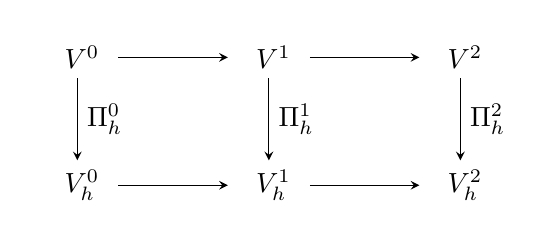
\begin{tikzpicture}[ampersand replacement=\&, baseline] %=(current  bounding  box.center)]
	\matrix (m) [matrix of math nodes,row sep=3em,column sep=4em,minimum width=2em] {
					~~ V^0 ~ \bbb
							\& ~~ V^1 ~ \bbb
									\& ~~ V^2 ~ \bbb
		\\
		~~ V^0_h ~ \bbb
				\& ~~ V^1_h ~ \bbb
						\& ~~ V^2_h ~ \bbb
		\\
	};
	\path[-stealth]
	(m-1-1) edge node [above] {$\grad$} (m-1-2)
					edge node [right] {$\Pi^0_h$} (m-2-1)
	(m-1-2) edge node [above] {$\curl$} (m-1-3)
					edge node [right] {$\Pi^1_h$} (m-2-2)
	(m-1-3) edge node [right] {$\Pi^2_h$} (m-2-3)
	(m-2-1) edge node [above] {$\grad$} (m-2-2)
	(m-2-2) edge node [above] {$\curl$} (m-2-3)
	;
	\end{tikzpicture}
\end{equation}

%TODO: mention that our construction also applies to the spaces with homogeneous boundary conditions.

On a single patch $\Omega_k$, %tensor-product space $V^{\ell}_k$, %of the form $\Omega_k = F_k(\hat \Omega)$, with 
the approach of \cite{buffa_isogeometric_2011} starts 
from a general tensor-product projection $\hat \Pi^0_k : L^2(\hat \Omega) \to \hat V^0_k$ 
on the first logical space, and defines
% pushing forward
% commuting 
projections on the next spaces %$\hat V^{\ell}_k$,
% built using the 
% tensor-product structure of the parametric spaces.
% Starting from a %can be mapped using the push-forward starts from a 
% stable projection 
% the method of \cite{buffa_isogeometric_2011} defines 
% and yields 
of the form 
\begin{equation}
	\label{Pi12k}
	\hat \Pi^1_k \hat \bu := \sum_{d \in \{1,2\}} \nabla_d \hat \Pi^0_k \hat \Phi_d(\hat \bu)
	\quad \text{ and } \quad
	\hat \Pi^2_k \hat f := \partial_1\partial_2 \hat \Pi^0_k \hat \Psi(\hat f)
\end{equation}
with antiderivative operators
\begin{equation*}
	\left\{\begin{aligned}
	\hat \Phi_1(\hat \bu)(\hbx) := \int_{0}^{\hx_1} \hat u_1(z, \hx_2) \dd z
	\\
	\hat \Phi_2(\hat \bu)(\hbx) := \int_{0}^{\hx_2} \hat u_2(\hx_1, z) \dd z	
\end{aligned}\right.
	\quad \text{ and } \quad
	\hat \Psi(\hat f)(\hbx) := \int_{0}^{\hx_1}\int_{0}^{\hx_2} \hat f(z_1,z_2) \dd z_2\dd z_1.
\end{equation*}
% where $\hat \bu$ and $\hat f$ are the 1-form and 2-form pull-backs of $\bu$ and $f$,
% respectively.
The projections \eqref{Pi12k} commute with the logical differential operators
thanks to the tensor-product structure of $\hat \Pi^0_k$, and they inherit 
its local stability due to the intrinsic integrability 
of the antiderivative operators.
On the mapped spaces the projections are defined through pull-backs and push-forwards,
\begin{equation*}
	\Pi^{\ell}_k = \cF^\ell_k \hat \Pi^{\ell}_k (\cF^\ell_k)^{-1} :
	\quad L^2(\Omega_k) \to V^\ell_k.
\end{equation*}
Their stability and commuting properties respectively follow from the smoothness of the mapping $F_k$ and from the fact that the pull-backs commute with the differential operators, see e.g. \cite{Hiptmair.2002.anum,buffa_isogeometric_2011}.

At patch interfaces where the parametric tensor-product structure breaks down, this construction must be adapted.
% \subsection{A broken-FEEC approach with interface correction terms}
Our approach is to first consider the patch-wise projections
\begin{equation} \label{Pipw}
\Pi^\ell_\pw = \sum_{k \in \cK} \Pi^\ell_k : \quad L^2(\Omega) \to V^{\ell}_\pw
\end{equation}
on the broken (fully discontinuous) patch-wise spaces
\begin{equation} \label{Vpw}
	V^{\ell}_\pw = 
		\{ v \in L^2(\Omega) : v|_{\Omega_k} \in V^{\ell}_k  \text{ for } k \in \cK\}
\end{equation}
% which are defined as the simple juxtaposition of the single-patch ones. 
% with a logical tensor-product structure.
and to modify the former so as to enforce the conformity conditions at the patch interfaces.
On the first space where the $H^1$ conformity amounts to continuity conditions, i.e.,
$V^0_h = V^0_\pw \cap C^0(\Omega)$,
this is done by applying a local conforming projection 
$P^0: V^0_\pw \to V^0_h$
which averages interface degrees of freedom: we set  %conforming projection 
\begin{equation}
\label{Pi0_intro}
\Pi^0_h := P^0 \Pi^0_\pw.
\end{equation}
On the next spaces our modification takes the form of additive correction terms
associated with the patch interfaces. The global projection on $V^1_h$ reads
% patch-wise projection, of the form
\begin{equation}
	\label{Pi1_intro}
	\Pi^1_h := \Pi^1_\pw 
		% \sum_{k \in \cK} \Pi^1_k 
			+ \sum_{e \in \cE} \tilde \Pi^1_e
					+ \sum_{\bv \in \cV} \tilde \Pi^1_\bv
						+ \sum_{\bv \in \cV, e \in \cE(\bv)} \tilde \Pi^1_{e,\bv}
\end{equation}
with correction terms %$\tilde \Pi^1_g : L^2(\Ome)$ with $g = e, \bv$ or $(e,\bv)$ are 
that are localized on patch edges and vertices. Like the single-patch
projections \eqref{Pi12k} they involve antiderivative operators,
local projections $\Pi^0_k$ and partial derivative operators. In addition they
also involve local projection operators which vanish on conforming functions. 
Specifically, our correction terms take the following form:
\begin{equation}
	\label{tPi1_intro}
	\left\{\begin{aligned}
	\tilde \Pi^1_e \bu &:= \sum_{d \in \{\parallel, \perp\}} \nabla^e_d (P^e - I^e) \Pi^0_\pw \Phi^e_{d}(\bu)
	\\
	\tilde \Pi^1_\bv \bu &:= \nabla_\pw (P^{\bv} - \bar I^{\bv}) \Pi^0_\pw \Phi^\bv(\bu)
	\\[5pt]
	\tilde \Pi^1_{e,\bv} \bu &:= \sum_{d \in \{\parallel, \perp\}} 
						\nabla^e_d (\bar I^e_{\bv} - P^e_{\bv})\Pi^0_\pw \Phi^{\bv,e}_{d}(\bu).
	\end{aligned}
\right.
\end{equation}
Here, $\nabla_\pw$ is the patch-wise gradient operator and 
$\nabla^e_d$, $d \in \{\parallel,\perp\}$, 
are patch-wise gradients along the logical parallel and perpendicular 
directions relative to a given edge $e$: they will be defined in Section~\ref{sec:broken}.
The various operators $P^g$, $I^g$, $\bar I^g$ ... are 
discrete projections on local conforming and broken subspaces associated to patch
edges (for $g = e$), vertices (for $g = \bv$) and edge-vertex pairs (for $g = (\bv,e)$). 
These local projection operators are designed so as to guarantee the grad-commuting properties 
of $\Pi^1_h$ and $\Pi^0_h$, and to vanish on continuous functions: they 
will be described in Section~\ref{sec:conf}.
Finally the various $\Phi^g$ operators are antiderivative operators associated 
with edges and vertices: they will be studied in Section~\ref{sec:antider}. 

Similarly, the projection on $V^2_h$ reads
\begin{equation}
	\label{Pi2_intro}
	\Pi^2_h :=
		\Pi^2_\pw 
			+ \sum_{e \in \cE} \tilde \Pi^2_e
						+ \sum_{\bv \in \cV, e \in \cE(\bv)} \tilde \Pi^2_{e,\bv}
\end{equation}
with interface correction terms of the form
\begin{equation}
	\label{tPi2_intro}
	\left\{\begin{aligned}
	\tilde \Pi^2_e f & := D^{2,e} (P^e - I^e) \Pi^0_\pw \Psi^{e}(f)
	\\
	% \\[5pt]
	\tilde \Pi^2_{e,\bv} f & := 
					D^{2,e} 
						(\bar I^e_{\bv} - P^e_{\bv})\Pi^0_\pw \Psi^{\bv,e}(f).	
	\end{aligned}
\right.
\end{equation}
Here, $D^{2,e}$ is a second order patch-wise derivative and 
$\Psi^{e}$, $\Psi^{\bv,e}$ are bivariate antiderivative: they will be 
described in Section~\ref{sec:broken} and \ref{sec:antider}.

Our findings can be summarized as follows. %that this construction yields following theorem.

% Our main result is 
\begin{theorem}
	The operators $\Pi^\ell_h$ 
	are local projections on the spaces $V^\ell_h$, $\ell = 0, 1, 2$.
	They yield a commuting diagram \eqref{cd}
	and they are uniformly $L^2$ stable
	with respect to the %constants independent of the 
	size and inner resolution
	of the patches.
\end{theorem}


% To overcome this difficulty we begin by summing the single patch projection 
% operators $\Pi^1_k$ that
% design our projection operator on $V^1_h$ 
% by adding correction terms corresponding to the different interfaces to the 
% single patch operators $\Pi^1_k$. 
% 
% adding correction terms
This result will be formally stated and proven in Section~\ref{sec:cpo}.
Here a precise meaning for the uniform stability will be given by 
listing discretization parameters 
$\kappa_1$, $\kappa_2$, $\dots$ on which our estimates depend:
they will characterize the regularity of our multipatch spaces.
Throughout the article we will then write 
\begin{equation*}
f \lesssim g
\end{equation*}
to mean that $f \le C g$ holds for a constant that only depends on these constants $\kappa_m$ 
while $f \sim g$ indicates that both $f \lesssim g$ and $g \lesssim f$ hold.




%%%% %%%% %%%% %%%% %%%% %%%% %%%% %%%% %%%% %%%% %%%% %%%% %%%% %%%% %%%% %%%% 
%%%% %%%% %%%% %%%% %%%% %%%% %%%% %%%% %%%% %%%% %%%% %%%% %%%% %%%% %%%% %%%% 

\section{Broken multipatch spaces}
\label{sec:broken}

In this section we describe in more detail the multipatch domain 
and the finite element spaces on which our construction applies.


\subsection{Multipatch geometry}
\label{sec:geom}

As described above we consider a domain $\Omega$ 
of the form \eqref{Om}, made of disjoint open patches
$\Omega_k = F_k(\hat \Omega)$ with smooth mappings
$F_k$, $k \in \cK$.
We denote by $H_k$ the diameter of patch $\Omega_k$, 
and assume that the mappings are $C^1$ diffeomorphisms
with Jacobian matrices satisfying
\begin{equation*}
% \kappa_1 \le 
\norm{DF_k} \le \kappa_1 H_k 
\quad \text{ and } \quad
\norm{(DF_k)^{-1}} \le \kappa_2  (H_k)^{-1}
\qquad \text{ for all } k \in \cK.
\end{equation*}
In particular, %we see that the bounds \eqref{boundsDF} yield
\begin{equation}  \label{boundsDF}
\norm{DF_k} \sim H_k, 
\quad 
\norm{(DF_k)^{-1}} \sim (H_k)^{-1}, 
\quad
\det (DF_k) \sim H_k^2 %, \qquad . 
\end{equation}
hold for all $k \in \cK$.
We make the following assumptions: 
\begin{itemize}
	\item[(i)] 
	the decomposition is geometrically conforming,
	\item[(ii)] across an edge $e \in \cE$ the patch discretizations are either the same or nested,
	\item[(iii)] vertices $\bv \in \cV$ may be shared by at most four patches 
	(exactly four in the case of interior vertices)
	with one coarse edge.
\end{itemize}
Here, (i) amounts to saying that the intersection of two closed patches 
is either empty, or a common vertex $\bv$, or a common edge $e$. In addition 
we assume that the mappings are continuous on the patch edges, in the sense that
both sides provide the same parametrization up to a possible change in orientation.
The precise meaning of assumptions (ii) and (iii) will be specified in Section~\ref{sec:ev}.


 
\subsection{Tensor-product logical spaces} %Primal and dual bases}

Following \cite{Hiptmair.2002.anum,buffa_isogeometric_2011,perse_geometric_2021}, 
we consider discrete spaces on each patch which are obtained by pushing forward 
tensor-product de Rham sequences on the logical cartesian domain $\hat \Omega$.

To allow for local refinements,
each logical patch is equipped with a local discrete de Rham sequence 
\begin{equation*}
\hat V^{0}_{k}
~ \xrightarrow{ \grad }  ~
\hat V^{1}_{k} 
~ \xrightarrow{ \curl}  ~
\hat V^{2}_{k} 
\end{equation*}
with tensor-product spaces of the form
\begin{equation*}
\hat V^{0}_{k}  := \VV^{0}_k \otimes \VV^{0}_k,
\qquad
\hat V^{1}_{k}  := \begin{pmatrix}
  \VV^{1}_{k} \otimes \VV^{0}_k
  \\ \noalign{\smallskip}
  \VV^{0}_k\otimes \VV^{1}_{k}
\end{pmatrix},
\qquad
\hat V^{2}_{k}  := \VV^{1}_{k} \otimes \VV^{1}_{k}.
\end{equation*}
% TODO: check, and add this remark if true
% \begin{remark}
% 	Our assumption that the discretization is isotropic in every patch 
% 	is to avoid additional complexity in the notations.
% 	Our construction, however, remains valid for anisotropic patch discretizations.
% \end{remark}
Here the univariate spaces form de Rham sequences on the reference interval, 
i.e.,
\begin{equation} \label{1D_seq}
\VV^{0}_{k} \subset W^{1,1}([0,1])
\quad \xrightarrow{ \mbox{$~ \partial_\hx ~$}}  \quad 
\VV^{1}_{k} \subset L^1([0,1])
\end{equation} 
% holds for both logical dimensions $d \in \{\hx, \hy\}$, 
and antiderivative operators map back to the first space,
\begin{equation} \label{ad_1d}
	\VV^{0}_{k}
	\quad \xleftarrow{ \mbox{$~ \int^{\hx} ~$}}  \quad 
	\VV^{1}_{k}
\end{equation}
for arbitrary integration constants,
which also implies that constants belong to $\VV^{0}_{k}$.
An important particular case is provided by spline spaces 
\begin{equation*}
	\VV^{0}_{k} = \mathbbm{S}^p_{\bs\alpha},  \qquad
	\VV^{1}_{k} = \mathbbm{S}^{p-1}_{{\bs\alpha} - 1} 
\end{equation*}
where $p$ and ${\bs\alpha}$ are the degree and regularity vector of the first space, 
as described in \cite{buffa_isogeometric_2011}. We remind that this also includes
the case of polynomial spaces, namely $\VV^{0}_{k} = \PP^p$ and $\VV^{0}_{k} = \PP^{p-1}$. 
To simplify the matching of functions across patch interfaces we further assume that 
the univariate spaces are invariant by a change of orientation, namely
\begin{equation} \label{sym_VV0}
  \vp \in \VV^{0}_{k} \quad \implies \quad \vp \circ \eta \in \VV^{0}_{k}
	\quad \text{where} \quad \eta(s) = 1-s.
\end{equation}

Our next assumption is that the first space is equipped with basis functions 
\begin{equation*}
\VV^{0}_{k} = \Span(\{\lambda^{k}_{i} : i = 0, \dots, n_k\})
\end{equation*}
with the following properties:
\begin{itemize}
	\item an interpolation property at the endpoints,
	\begin{equation} \label{ipe}
		\lambda^{k}_{i}(0) = \delta_{i,0}
		\qquad \text{ and } \qquad
		\lambda^{k}_{i}(1) = \delta_{i,n_k}
	\end{equation}

	\item bounded overlapping and quasi-uniformity:
	the open supports of $\lambda^{k}_i$, which we denote by $\hat S^{k}_i$,
	are intervals of diameter 
	\begin{equation} \label{S_size}
		\kappa_3^{-1} \hat h_k \le \diam(\hat S^{k}_i) \le \kappa_3 \hat h_k
		\qquad \text{with} \qquad 
		\hat h_k := (n_k+1)^{-1}
	\end{equation}
	and they overlap in a bounded way, i.e.
	\begin{equation} \label{overlap}
		\#\big(\{ j : \hat S^{k}_j \cap \hat S^{k}_i \neq \emptyset \}\big)
		\le \kappa_4
		\qquad
		\text{ for } i = 0, \dots, n_k.
	\end{equation}

	\item inverse estimate:	
	assuming an $L^\infty$ normalization, we have the estimate
	\begin{equation} \label{l_norm}
		\norm{\lambda^{k}_{i}}_{L^\infty} \le 1,
			\qquad 		
		\norm{\partial_\hx \lambda^{k}_{i}}_{L^\infty} 
			\le \kappa_5 (\hat h_k)^{-1}.
		\end{equation}

	\item local stability:
	there exists dual basis functions $\theta^{k}_{i}$ 
	with the same supports $\hat S^{k}_{i}$ (for simplicity), such that
	\begin{equation*}
	\sprod{\theta^{k}_{i}}{\lambda^{k}_j}_{L^2([0,1])} = \delta_{i,j}
	% \quad \text{ for }
	\end{equation*}
	holds for all $i, j \in \{0, \dots, n_k\}$, as well as
	the normalization %(for all $i \in \{0, \dots, n_k\}$)
	\begin{equation} \label{t_norm}
		\norm{\theta^{k}_{i}}_{L^\infty} \le \kappa_6 (\hat h_k)^{-1}.
	\end{equation}

\end{itemize}
%
The basis functions for $\hat V^0_k$, as well as the dual functions, are 
then defined as 
\begin{equation*}
\left\{\begin{aligned}
	\hat \Lambda^{k}_{\bi}(\hbx) := \lambda^{k}_{i_1}(\hx_1) \lambda^{k}_{i_2}(\hx_2)
	\\
	\hat \Theta^{k}_{\bi}(\hbx) := \theta^{k}_{i_2}(\hx_1) \theta^{k}_{i_2}(\hx_2)
\end{aligned}\right.
\qquad \text{ for } ~
\hbx \in \hat \Omega, \quad \bi \in \cI^k := \{0, \dots, n_k\}^2.
\end{equation*}
Both functions have the same supports 
\begin{equation} \label{hSki}
\hat S^{k}_{\bi} = \hat S^{k}_{i_1} \times \hat S^{k}_{i_2}
\end{equation}
which, according to \eqref{overlap}, also overlap in a bounded way.
From \eqref{S_size} and the normalization \eqref{l_norm}, \eqref{t_norm} we infer
\begin{equation} \label{hLT_L2}
	% \left\{\begin{aligned}
	\norm{\hat \Lambda^{k}_{\bi}}_{L^2(\hat S^k_\bi)} 
	%\lesssim \norm{\hat \Lambda^{k}_{\bi}}_{L^\infty} \abs{\hat S^k_\bi}^{\frac 12} 
	\lesssim \hat h_k,
	\qquad
% \end{equation}
% and 
% \begin{equation} \label{hTheta_L2}
	\norm{\hat \Theta^{k}_{\bi}}_{L^2(\hat S^k_\bi)} %\lesssim 
% \norm{\hat \Theta^{k}_{\bi}}_{L^\infty} \abs{\hat S^k_\bi}^{\frac 12}
	\lesssim (\hat h_k)^{-1}.
% \end{aligned}\right.
\end{equation}
%
Using these dual functions we can define a projection operator
\begin{equation} \label{hPi0k}
\hat \Pi^0_k: L^2(\hat \Omega) \to \hat V^0_k, \qquad 
\hat \phi \mapsto \sum_{\bi \in \cI^k} 
	\sprod{\hat \Theta^{k}_{\bi}}{\hat \phi}_{L^2(\hat \Omega)} \hat \Lambda^{k}_{\bi}.
\end{equation}
Our assumptions classically imply that both the basis and $\hat \Pi^0_k$ are locally stable. 
Specifically, if we define the {\em extension} of a domain 
$\hat \omega \subset \hat \Omega$ as
\begin{equation} \label{hEk_ext}
	\hat E_k(\hat \omega) := \bigcup_{\bi \in \cI^k(\hat \omega)} \hat S^k_\bi
	\quad \text{ where  } \quad
	\cI^k(\hat \omega) := 
		\{\bi \in \cI^k : \hat S^k_\bi \cap \hat \omega \neq \emptyset\},
\end{equation}
then we have 
\begin{equation} \label{stab_hPi0}
	\norm{\hat \Pi^0_k \hat \phi}_{L^2(\hat \omega)} 
		\lesssim \norm{\hat \phi}_{L^2(\hat E_k(\hat \omega))}		
		\qquad \text{ for } ~~ \hat \phi \in L^2(\hat \omega).
\end{equation}
To verify this we consider 
$\hat \phi_h = \sum_{k, \bi} \phi^k_\bi \hat \Lambda^{k}_\bi \in \hat V^0_k$, 
and use \eqref{hLT_L2} to estimate
\begin{equation} \label{stab_hbasis}
	\hat h_k \abs{\phi^k_\bi} 
	= \hat h_k \abs{\sprod{\hat \Theta^{k}_\bi}{\hat \phi_h}}_{L^2}
	\lesssim \norm{\hat \phi_h}_{L^2(\hat S^k_\bi)}
	\le \sum_{\bj \in \cI^k(\hat S^k_\bi)} \abs{\phi^k_\bj} \norm{\hat \Lambda^{k}_\bj}_{L^2}
	\lesssim \sum_{\bj \in \cI^k(\hat S^k_\bi)} \abs{\phi^k_\bj} \hat h_k
\end{equation}
which shows that the basis is indeed stable. Similarly we compute for $\hat \phi \in L^2(\hat \Omega)$
\begin{equation*}
% \begin{aligned}
	\norm{\hat \Pi^0_k \hat \phi}_{L^2(\hat \omega)}
	\le \sum_{\bi \in \cI^k(\hat \omega)} 
	\abs{\abs{\sprod{\hat \Theta^{k}_\bi}{\hat \phi}}_{L^2}} \norm{\hat \Lambda^{k}_\bi}_{L^2} 
	\lesssim \sum_{\bi \in \cI^k(\hat \omega)}  \norm{\hat \phi}_{L^2(\hat S^k_\bi)}
\end{equation*}
so that \eqref{stab_hPi0} follows from the bounded overlapping property 
\eqref{overlap} of the supports. 
Using \eqref{l_norm} we further infer 
$\norm{\nabla \hat \Lambda^{k}_\bi}_{L^2} \lesssim 1$
which yields the inverse estimate 
\begin{equation} \label{inverse_est}
	\norm{\nabla \hat \phi}_{L^2(\hat \omega)} 
			\lesssim \sum_{\bi \in \cI^k(\hat \omega)} \abs{\phi_\bi} \norm{\nabla \hat \Lambda^{k}_\bi}_{L^2}
			\lesssim \sum_{\bi \in \cI^k(\hat \omega)} \abs{\phi_\bi} 
			\lesssim (\hat h_k)^{-1}\norm{\hat \phi}_{L^2(E_h(\hat \omega))}. 
\end{equation}

A key property of the tensor-product structure is the well-known preservation of 
directional invariance.
\begin{lemma} \label{lem:dd_Pi0k}
	If $\partial_d \hat \phi = 0$ for some dimension $d \in \{1,2\}$,
	then $\partial_d \hat \Pi^0_k \hat \phi = 0$.
\end{lemma}
\begin{proof}
	% Let us write $\hat \psi \hat \phi(\bx)$
	Wlog consider the case $d=1$ so that $\hat \phi(\hbx) = \hat \phi(\hx_2)$, and compute 
	% The tensor-product structure of \eqref{hPi0k} allows us to write
	% for $\hat \psi(\hbx) := \hat \phi^k(0, \hx_{d'})$,
	\begin{equation*}
	\begin{aligned}
		\hat \Pi^0_k \hat \phi(\hbx)
			= \sum_{\bi \in \cI^k} \sprod{\hat \Theta^{k}_{\bi}}{\hat \phi} %_{L^2(\hat \Omega)} 
			\hat \Lambda^{k}_{\bi}(\hbx)
			= 
				\underbrace{\Big(\sum_{i_1} \sprod{\theta^{k}_{i_1}}{1} \lambda^{k}_{i_1}(\hx_1) \Big)}_{=~1}
				\Big(\sum_{i_2} \sprod{\theta^{k}_{i_2}}{\hat \phi} \lambda^{k}_{i_2}(\hx_2)\Big)
	\end{aligned}
	\end{equation*}
	where the univariate $L^2$ products are over $[0,1]$ and the last equality follows from the fact that 
	the first term in the product is the projection of a constant which belongs to all the univariate
	spaces $\hat \VV^{0}_{k}$. This shows that $\partial_d \hat \Pi^0_k \hat \phi = 0$ holds indeed.
\end{proof}
% \begin{lemma} \label{lem:dirinv_Pi0k}
% 	If $\hat \vp \in L^2(\hat \Omega)$ is such that $\hat \nabla_d \hat\vp = 0$,
% 	then,
% 	\begin{equation*}
% 	\hat\nabla_d \hat \Pi^0_k \hat \vp = 0.
% 	\end{equation*}
% \end{lemma}


% 
% ADD assumptions on basis functions normalization in V1 and locality od derivative...
% \begin{equation*}
% \norm{\lambda^{1,k}_{i}} \lesssim 1
% % \partial_{\hx} \lambda^{k}_{i} =  - \lambda^{1,k}_{i+1}
% \end{equation*}
% % where we have set $\lambda^{1,k}_{1} := 0$ for $\alpha \notin \{1, \dots, n_k\}$.




\subsection{Push-forward spaces on the mapped patches}

On each patch $\Omega_k = F_k(\hat \Omega)$,
the local spaces are defined as the image of the logical ones by 
the push-forward operators associated with $F_k$, i.e. 
$V^{\ell}_k := \cF^{\ell}_k (\hat V^{\ell}_{k})$.
We remind that these operators read
\begin{equation} \label{pf_gc}
  \left\{
  \begin{aligned}
  &\cF^0_k : \hat \phi \mapsto \phi := \hat \phi \circ F_k^{-1}
  \\
  &\cF^1_k : \hat \bu \mapsto \bu :=  \big(DF_k^{-T} \hat \bu \big)\circ F_k^{-1}
  \\
  &\cF^2_k : \hat f \mapsto f :=  \big(J_{F_k}^{-1} \hat f \big)\circ F_k^{-1}
  \end{aligned}
  \right.
\end{equation}
where $DF_k = \big(\partial_b (F_k)_a(\hat \bx)\big)_{1 \le a,b \le 2}$
is the Jacobian matrix of $F_k$, and $J_{F_k}$ %(\hat \bx) = \det (DF_k(\hat \bx))$
its (positive) metric determinant, 
see e.g. \cite{Hiptmair.2002.anum,kreeft2011mimetic,Buffa_Doelz_Kurz_Schoeps_Vazquez_Wolf_2019,%
Holderied_Possanner_Wang_2021}.
These operators define isomorphisms between $L^2(\hat \omega)$ and 
$L^2(\omega)$ for any open domain $\hat \omega \subset \hat \Omega$ 
with image $\omega = F_k(\hat \omega)$. Specifically, for all 
$\hat \phi, \hat \bu, \hat f \in L^2(\hat \Omega)$
the push-forwards
$\phi := \cF^0_k \hat \phi$, $\bu := \cF^1_k \hat \bu$ and  $f := \cF^2_k \hat f$
satisfy
\begin{equation} \label{L2_scale_pf}
	\norm{\phi}_{L^2(\omega)} \sim H_k \norm{\hat \phi}_{L^2(\hat \omega)},
	\quad 
	\norm{\bu}_{L^2(\omega)} \sim \norm{\hat \bu}_{L^2(\hat \omega)},
	\quad 
	\norm{f}_{L^2(\omega)} \sim H_k^{-1} \norm{\hat f}_{L^2(\hat \omega)}.
\end{equation}
A key property is the commutation with the differential operators, 
namely
\begin{equation*}
\grad \cF^0_k \hat \phi = \cF^1_k \grad \hat \phi,
\qquad 
\curl \cF^1_k \hat \bu = \cF^2_k \curl \hat \bu
\end{equation*}
which holds for all $\hat \phi \in H^1(\hat \Omega)$ and 
$\hat \bu \in H(\hcurl; \hat \Omega)$.
In particular the mapped spaces also form de Rham sequences
\eqref{dR_k}.



\subsection{Broken basis functions and patch-wise projection on $V^0_\pw$} 

Basis functions for the single-patch spaces $V^\ell_k = \cF_k^\ell \hat V^\ell_k$ 
are obtained by pushing forward the reference basis functions.
% $\Lambda^{\ell,k}_{\bi} := \cF^\ell_k(\hat \Lambda^{\ell,k}_{\bi})$,
Outside of $\Omega_k$ we implicitely extend $\cF^\ell_k$ by zero, so that
these functions also provide a basis for the patch-wise spaces \eqref{Vpw}.
Of particular importance to us is the corresponding basis for $V^{0}_\pw$,
\begin{equation*}
\Lambda^{k}_{\bi} := \cF^0_k(\hat \Lambda^{k}_{\bi})
	=
	\begin{cases}
		\hat \Lambda^{k}_{\bi} ~ &\text{ on } \Omega_k
		\\
		0 &\text{ elsewhere}
	\end{cases}
	\quad \text{ for } k \in \cK, \quad \bi \in \cI^k = \{0, \dots, n_k\}^2
\end{equation*} 
with local supports mapped from \eqref{hSki},
\begin{equation} \label{Ski}
S^{k}_\bi := F_k(\hat S^{k}_\bi) = \supp(\Lambda^{k}_{\bi}) \subset \Omega_k.
\end{equation} 
The stability of the basis follows from \eqref{stab_hbasis}, \eqref{L2_scale_pf}:
for $\phi_h = \sum_{k, \bi} \phi^k_\bi \Lambda^{k}_\bi \in V^0_k$, 
\begin{equation} \label{stab_basis}
	h_k \abs{\phi^k_\bi}
		\lesssim \norm{\phi_h}_{L^2(S^k_\bi)} 
			\lesssim h_k \sum_{\bj \in \cI^k(\hat S^k_\bi)} \abs{\phi^k_\bj}		
\end{equation}
holds with  
\begin{equation} \label{hk}
	h_k := H_k \hat h_k = \frac{\diam(\Omega_k)}{n_k + 1}. 
%see  from \eqref{Hk} and \eqref{S_size} % \hat h_k := \frac {1}{n_k}.	
\end{equation}
% Using \eqref{S_size} this also yields
% \begin{equation} \label{bound_L}
% 	\norm{\Lambda^{k}_\bi} \sim h_k \sim \diam(S^{k}_\bi),
% 	\qquad k \in \cI^k.
% \end{equation}
The single-patch projection operator is then defined as
\begin{equation} \label{Pi0k}
	\Pi^0_k = \cF^0_k \hat \Pi^0_k (\cF^0_k)^{-1}
\end{equation}
% where $\hat \Pi^0_k$ is the reference 
see \eqref{hPi0k},
and the patch-wise projection on $V^0_\pw$ consists of summing the local contributions,
\begin{equation} \label{Pi0pw}
	\Pi^0_\pw = \sum_{k \in \cK} \Pi^0_k : \quad L^2(\Omega) \to V^0_\pw.
\end{equation}

\begin{lemma} \label{lem:stab_Pi0k}
	On a domain $\omega \subset \Omega_k$, $k \in \cK$,
	the single-patch projection satisfies
	\begin{equation} \label{stab_Pi0k}
		\norm{\Pi^0_k \phi}_{L^2(\omega)} 
			\lesssim \norm{\phi}_{L^2(E_k(\omega))}		
			\qquad \text{ for } ~~ \phi \in L^2(\omega)
	\end{equation}
 	with $E_k(\omega)$ the single-patch extension corresponding to \eqref{hEk_ext},
	\begin{equation} \label{Ek_ext}
		E_k(\omega)			
			:= F_k(\hat E_k(F_k^{-1}(\omega)))
			= \bigcup_{\bi \in \cI^k: \, S^k_\bi \cap \omega \neq \emptyset} S^k_\bi,
	\end{equation}
	which is also visualized in Figure \ref{fig:dom_ext_patch}.
	In particular, for any constant $c$ we have
	\begin{equation} \label{c_Pi0}
	\phi = c \text{ on } E_k(\omega) \quad \implies \quad \Pi^0_k \phi = c \text{ on } \omega
	\end{equation}
	and the patch-wise projection satisfies the global bound
	\begin{equation} \label{stab_Pi0_pw}
		\norm{\Pi^0_\pw \phi}_{L^2(\Omega)} \lesssim \norm{\phi}_{L^2(\Omega)}.		
	\end{equation}
\end{lemma}
\begin{proof}
	The bound \eqref{stab_Pi0k} follows by applying \eqref{stab_hPi0} 
	to the pull-back $\hat \phi = (\cF_k^0)^{-1}\phi$ 
	and using the scaling properties \eqref{L2_scale_pf}.
	To show \eqref{c_Pi0} we apply this bound
	to the function $\psi = \phi - c$ and use the fact that $\Pi^0_k c = c$
	holds because the constants belong to $\hat V^0_k$, hence also to $V^0_k$.
	(In passing note that \eqref{c_Pi0} holds for all functions $c \in V^0_k$,
	not only constants.)
	Estimate \eqref{stab_Pi0_pw} then follows 
	by summing the local bounds \eqref{stab_Pi0k} over $k \in \cK$ 
	with $\omega = \Omega_k$ (whose domain extension is $E_k(\Omega_k) = \Omega_k$)
	and by using the fact that the patches form a partition the domain $\Omega$.
\end{proof}

\begin{comment}
	
	This basis is locally $L^2$ stable in the sense that for
an arbitrary $\phi = \sum_{k, \bi} \phi^k_\bi \Lambda^{k}_\bi$ in the broken space 
$V^0_\pw$, we have
\begin{equation} \label{stab_basis}
 	h_k \abs{\phi^k_\bi} \lesssim \norm{\phi}_{L^2(S^k_\bi)} \lesssim h_k \sum_{\bj \in \cI^k(S^k_\bi)} \abs{\phi^k_\bj}
\end{equation}
holds for all $k$ and $\bi \in \cI^k$, with 
$\cI^k(S^k_\bi) = \{ \bj \in \cI^k : S^k_\bj \cap S^k_\bi \neq \emptyset \}$ 
as defined in \eqref{Ek_ext}.
Indeed from the scaling properties of the basis 
and dual functions \eqref{hLT_L2}, we have
\begin{equation*}
\abs{\phi^k_\bi} = \abs{\sprod{\hat \Theta^{k}_\bi}{\hat \phi}} 
\lesssim \hat h_k^{-1} \norm{\hat \phi}_{L^2(\hat S^k_\bi)}
\end{equation*}
moreover
\begin{equation*}
\norm{\hat \phi}_{L^2(\hat S^k_\bi)} 
\le \sum_{\bj \in \cI^k(S^k_\bi)} \abs{\phi^k_\bj} \norm{\hat \Lambda^{k}_\bj}_{L^2(\hat S^k_\bi)}
\lesssim \sum_{\bj \in \cI^k(S^k_\bi)} \abs{\phi^k_\bj} \hat h_k.
\end{equation*}
The estimate \eqref{stab_basis} follows from the scaling property of 0-form pullbacks
\eqref{L2_scale_pf}.
\end{comment}


\begin{figure}
	\centering 
	 {
		\fontsize{13pt}{18pt}\selectfont
	 \resizebox{!}{0.25\textheight}{\input{plots/dom_ext_p.pdf_tex}}
		}
	\caption{Domain extensions of a domain % and mapped patches. 
	$\hat \omega \in \hat \Omega$ (left) 
	and its mapped image $\omega = F_k(\hat \omega)$ on a patch $\Omega_k$ (right), 
	as defined by equations \eqref{hEk_ext} and \eqref{Ek_ext}. 
	In different shading we show the overlapping basis function supports 
	$\hat S^{k}_\bi$ and $S^{k}_\bi$ that have a non-empty intersection with 
	the respective $\hat \omega$ and $\omega$. The domain extensions 
	$\hat E_k(\hat \omega)$ and $E_k(\omega)$ are the domains delimited by
	the orange boundaries.
	 % On the right, we show the equivalent mapped quantities $\omega$, $S^{k}_\bi$ 
	% and $E_k(\omega)$ in a similar setup.
	}
	\label{fig:dom_ext_patch}
\end{figure}

\subsection{Edges and vertices}
\label{sec:ev}

We denote by $\cE$ the set of patch edges. 
Given $e \in \cE$, the indices of contiguous patches is gathered in the set
\begin{equation*}
\cK(e) = \{k \in \cK: e \subset \partial \Omega_k\}.
\end{equation*}
Our edge-nestedness assumption (ii) from Section~\ref{sec:geom} is that $\cK(e)$
consists either of two patches $k^-(e)$, $k^+(e)$ of nested resolutions
in the sense that 
\begin{equation} 
	\label{-+_assumption}
	\VV^{0}_{k^-(e)} \subset \VV^{0}_{k^+(e)},
\end{equation}
or of a single patch (if $e \subset \partial \Omega$), 
which we also denote by $k^-(e)$.

Moreover we assume that two adjacent patches across an edge $e$ have similar
diameters and resolutions, i.e.,
\begin{equation}\label{sdr}
	\kappa_7^{-1} \le \frac{H_{k^-(e)}}{H_{k^+(e)}} \le \kappa_7
	\quad \text{ and } \quad
	\kappa_8^{-1} \le \frac{n_{k^-(e)}}{n_{k^+(e)}} \le \kappa_8.
\end{equation}
Given an edge $e$ and a point $\bx \in \Omega_k$, $k \in \cK(e)$,
we denote by $(\hx^k_{\parallel}, \hx^k_{\perp})$
(with implicit dependence on $e$)
the components of the reference variable $\hbx = (\hx_1, \hx_2) := F_k^{-1}(\bx)$ 
in the directions parallel and perpendicular to the 
reference edge $\hat e^k := (F_k)^{-1}(e)$. 
In other terms, we set
\begin{equation} \label{ppe}
(\hx^k_{\parallel}, \hx^k_{\perp}) = (\hx^k_{\parallel(e)}, \hx^k_{\perp(e)}) %:= 
:= \begin{cases}
	(\hx_1, \hx_2) & \text{ if $\hat e^k$ is parallel to the $\hx_1$ axis}
	\\
	(\hx_2, \hx_1) & \text{ if $\hat e^k$ is parallel to the $\hx_2$ axis}
\end{cases}
\end{equation}
and it will be convenient to denote the corresponding reordering function by 
\begin{equation}
	\label{Xke}
	\hat X^k_e : (\hx^k_\parallel,\hx^k_\perp) \mapsto \hbx 
	\quad \text{ and } \quad 
	X^k_e := F_k (\hat X^k_e) : (\hx^k_\parallel,\hx^k_\perp) \mapsto \bx .
\end{equation}
% Note that this is always an involution, so that 
% $\hat X^k_e(\hx^k_\parallel,\hx^k_\perp) = \hbx$ also holds.
% In particular we may write $X^k_e := F_k(\hat X^k_e)$ when convenient.
Using this notation, a logical edge is always of the form 
\begin{equation} \label{e_perp}
	\hat e^k = \{\hbx \in \hat \Omega : \hx^k_\perp = \hat e^k_\perp\}
\end{equation}
where $\hat e^k_\perp \in \{0,1\}$ is constant for any $e$ and $k \in \cK(e)$.
We next let $\cV$ be the set of all vertices and for
$\bv \in \cV$ we gather the 
indices of the contiguous patches in the set
\begin{equation*}
\cK(\bv) = \{k \in \cK: \bv \in \partial \Omega_k\}. % \qquad  \bv \in \cV.
\end{equation*}

\begin{figure}[h]
	\centering 
	 {
	\fontsize{18pt}{22pt}\selectfont
	 \resizebox{!}{0.3\textheight}{\input{plots/vertex_partition.pdf_tex}}
		}
	\caption{Adjacent patches around a vertex $\bv$
	corresponding to the decomposition \eqref{cK_seqs}, with
	$n^l(\bv) =  n^r(\bv) = 2$ since $\bv$ is an interior vertex.
	%$\cK(\bv) = \{k^l_1(\bv), k^l_2(\bv) \} \cup \{k^r_1(\bv), k^r_{2}(\bv) \}$.
	Here the plotted cells correspond to the minimal intersections of the overlapping
	supports $S^{k}_\bi$ defined in \eqref{Ski}.
	}
	\label{fig:ver_part}
\end{figure}

Our assumption (iii) from Section~\ref{sec:geom}
consists of saying that $\cK(v)$ consists of two sequences
of adjacent patches with nested resolutions, namely
\begin{equation} \label{cK_seqs}
	\cK(\bv) = \{k^l_i(\bv) : 1 \le i \le n^l(\bv)\} \cup 
	\{k^r_i(\bv) : 1 \le i \le n^r(\bv)\}
\end{equation}
with two integers $n^l(\bv), n^r(\bv) \le 2$ %for $s = l$ or $r$,
%satisfying $n^l(\bv) + n^r(\bv) = \#(\cK(\bv))$
and $n^l(\bv)= n^r(\bv) = 2$ if $\bv$ is an interior vertex. 
(We may assume that one sequence rotates clockwise and the other one rotates counterclockwise.)
These patches are adjacent and nested in the following sense:
\begin{itemize}
	\item if both patches
	$\Omega_{k^s_1(\bv)}$ and $\Omega_{k^s_2(\bv)}$ exist (with $s = l$ or $r$)
	then they must share an edge which we denote by $e^s(\bv)$, 
	and %they are of nested resolution in the sense that 
	their FEM spaces satisfy
	\begin{equation*}
	\VV^{0}_{k^s_{1}(\bv)} \subset \VV^{0}_{k^s_{2}(\bv)} \quad \text{ for $s = l$ or $r$}
	\end{equation*}
	
	\item if both sequences are non-empty ($n^s(\bv) \ge 1$ for both $s = l$ and $r$), 
	then %we further assume that 
	the patches $k^l_1(\bv)$ and $k^r_1(\bv)$ must also 
	share an edge which is denoted $e^*(\bv)$.
\end{itemize}
Note that if only one sequence is non-empty ($n^s(\bv) \ge 1$ for either $s = l$ or $r$,
which can only happen for boundary vertices), 
then its first patch $k^s_1(\bv)$ has two edges contiguous to $\bv$ which we also 
denote by $e^s(\bv)$ and $e^*(\bv)$: if $n^s(\bv) = 2$ then $e^s(\bv)$ is shared by
two patches as described above while $e^*(\bv)$ is a boundary edge, 
and if $n^s(\bv) = 1$ then both edges are on the boundary.

In the sequel the edges $e^l(\bv)$ and $e^r(\bv)$ (when they exist) will be called
the left and right intermediate edges of $\bv$, while $e^*(\bv)$ 
(which always exists) will be called the coarse edge of $\bv$.
An example configuration can be seen in Figure \ref{fig:ver_part}. 

% (If $\bv$ is an interior vertex then the finest patches must also be adjacent.)
% \begin{definition} \label{def:v_orientation}	
% 	Let $\Omega_k$, $k \in \cK(\bv)$, be a patch contiguous to $\bv$, i.e. $k = k^s_i(\bv)$ with 
% 	$1 \le i \le N^s(\bv)$, $s = l$ or $r$.
% 	If $i < N^s(\bv)$ then we say that the interface $e' = \partial\Omega_{k} \cap \partial\Omega_{k'}$,
% 	with $k' = k^s_{i+1}(\bv)$,
% 	is the \textbf{fine interface} of $\Omega_k$.
% 	If $i = 1$ and if there exists a patch $k^* = k^{t}_1(\bv)$ in the other sequence $t \neq s$,
% 	or if $i > 1$ (in which case $k$ has a coarse neighboor $k^* = k^{s}_{i-1}(\bv)$), 
% 	then we say that the interface $e^* = \partial\Omega_{k} \cap \partial\Omega_{k^*}$
% 	is the \textbf{coarse interface} of $\Omega_k$.
% 	Finally we say that $\Omega_k$ has a \textbf{canonical orientation} 
% 	relative to the vertex $\bv$ if the following conditions are satisfied:
% 	\begin{itemize}
% 		\item [(i)] the local coordinates of the vertex are $(F_k)^{-1}(\bv) = (0,0)$, 
% 		\item [(ii)] if there is a fine interface, it corresponds to the 
% 		edge $(F_k)^{-1}(e') = \{\hx_2 = 0\}$,
% 		\item [(iii)] if there is a coarse interface, it corresponds to $(F_k)^{-1}(e^*) = \{\hx_1 = 0\}$.
% 	\end{itemize}
% \end{definition}



\subsection{Patch-wise differential operators}

Using the push-forward and pull-back operators we also define patch-wise gradient operators.
Given $d \in \{1,2\}$, we define the single-patch directional gradients as
\begin{equation} \label{nabla_kd}
	\nabla^k_d : V^{0}_k \to V^{1}_k, 
	\qquad \phi \mapsto \cF^1_k \big( \hat \btau_d \partial_{\hx_d} (\cF^0_k)^{-1}(\phi)
\end{equation}
where $\hat \btau_d$ is the unit vector of $\RR^2$ along $\hx_d$,
and the patch-wise (broken) gradient is
\begin{equation} \label{nabla_pw}
	\nabla_\pw : V^{0}_\pw \to V^{1}_\pw, 
	\qquad \phi \mapsto \sum_{k \in \cK, d \in \{1,2\}} \nabla^k_d (\phi|_{\Omega_k})
\end{equation}
(where each single-patch gradient is implicitely extended by zero outside of its patch).
Finally for an edge $e \in \cE$ we define broken gradients
along the parallel and perpendicular directions: for $d \in \{\parallel,\perp\}$,
\begin{equation} \label{nabla_ed}
	\nabla^e_d : V^{0}_\pw \to V^{1}_\pw,
	\quad
	\phi \mapsto \sum_{k\in \cK(e)} \cF^1_k \big( \hat \btau^k_d \partial_{\hx_d} (\cF^0_k)^{-1}(\phi|_{\Omega_k})\big)
\end{equation}
where $\hat \btau^k_d$ is the unit vector of $\RR^2$ along $\hx^k_d$, the 
parallel or perpendicular logical directions respective to $e$ according to \eqref{ppe}.
Observe that these operators satisfy
\begin{equation} \label{sum_nabla_ked}
	\nabla^e_\parallel + \nabla^e_\perp = \sum_{k \in \cK(e)} \nabla^k_1 + \nabla^k_2 = \nabla_\pw
	\quad 
	\text{ on } \quad \Omega(e) := \cup_{k\in \cK(e)} \Omega_k.
\end{equation}

To design our commuting projection on $V^2_h$ we will need 
broken second order (mixed) derivative operators:
a single patch operator %$$ defined as 
\begin{equation} \label{D2k}
	D^{2,k} := \cF_k^2 \hat \partial_1 \hat \partial_2 (\cF_k^0)^{-1}
	: \quad V^0_k \to V^2_k
	% D^{2,k} \phi|_{\Omega_k} 
	% 	:= \cF_k^2\big(\hat \partial_1 \hat \partial_2 \hat \phi^k \big)
\end{equation}
and a patch-wise operator $D^{2,e} : V^0_\pw \to V^2_\pw$ 
associated with any edge $e \in \cE$.
We define the latter by its values on the local domain $\Omega(e)$, as 
% patches $\Omega_k$, $k\in \cK(e)$, as
\begin{equation} \label{D2e}
	D^{2,e} \phi|_{\Omega_k} 
		:= (\det \hat X^k_e) \cF_k^2\big(\hat \partial^k_\parallel \hat \partial^k_\perp \hat \phi^k \big)
\end{equation}
where we have denoted $\hat \phi^k := (\cF_k^0)^{-1}\phi \in \hat V^0_k$.
Outside of $\Omega(e)$ we set $D^{2,e} \phi = 0$.
Note that $\det \hat X^k_e = \pm 1$ so that $D^{2,e} \phi|_{\Omega_k}$
indeed belongs to $V^2_k$.
This operator satisfies the following relation.
\begin{lemma} \label{lem:D2e}
	Let $\psi_\parallel$, $\psi_\perp$ be functions in $V^0_\pw$ which vanish
	outside $\Omega(e)$.
	We have 
	% The patch-wise curl of
	% reads
	\begin{equation*}
	\curl_\pw \Big(\sum_{d \in \{\parallel, \perp\}} \nabla^e_d \psi_d \Big)
	= D^{2,e} (\psi_\perp - \psi_\parallel).
	\end{equation*}
\end{lemma}
\begin{proof}
	Let $\bw := \sum_{d \in \{\parallel, \perp\}} \nabla^e_d \psi_d$.
	On each patch $\Omega_k$, $k \in \cK(e)$, its pull-back 
	 reads
	\begin{equation*}
	\hat \bw^k := (\cF_k^1)^{-1} \bw
	= \sum_{d \in \{\parallel, \perp\}} \hat \btau^k_d \hat \partial^k_d \hat \psi^k_d
	= \begin{cases}
		(\hat \partial^k_\parallel \hat \psi^k_\parallel, 
			\hat \partial^k_\perp \hat \psi^k_\perp ) & \text{ if } \det \hat X^k_e = 1
			\\
		(	\hat \partial^k_\perp \hat \psi^k_\perp,
		  \hat \partial^k_\parallel \hat \psi^k_\parallel ) & \text{ if } \det \hat X^k_e = -1
	\end{cases}
	\end{equation*}
	where we have denoted $\hat \psi^k_d := (\cF_k^0)^{-1} \psi_d$. 
	In particular, we have
	\begin{equation*}
	\begin{aligned}
		\curl_\pw \bw |_{\Omega_k}
		= \cF_k^2\big( \hcurl \hat \bw^k \big)
		= (\det \hat X^k_e) \cF_k^2\big(\hat \partial^k_\parallel \hat \partial^k_\perp (\hat \psi^k_\perp - \hat \psi^k_\parallel)\big)
		= D^{2,e} (\psi_\perp - \psi_\parallel) |_{\Omega_k}.
	\end{aligned}
	\end{equation*}	
\end{proof}




%%%% %%%% %%%% %%%% %%%% %%%% %%%% %%%% %%%% %%%% %%%% %%%% %%%% %%%% %%%% %%%% 
%%%% %%%% %%%% %%%% %%%% %%%% %%%% %%%% %%%% %%%% %%%% %%%% %%%% %%%% %%%% %%%% 

\section{Conforming multipatch spaces}
\label{sec:conf}

In this section we specify a basis for the first conforming space 
$V^0_h = V^0_\pw \cap H^1(\Omega)$, 
and we construct several projection operators on local broken and conforming 
spaces that will play a central role in the construction of our commuting operators,
as presented in Section~\ref{sec:approach}. % $\Pi^\ell_h$, $\ell = 0, 1, 2$.



\subsection{Conforming constraints on patch interfaces}

The finite element spaces \eqref{Vh} are the maximal conforming subspaces
of the broken spaces \eqref{Vpw}, namely
\begin{equation*} %\label{Vh_sub}
	V^0_h = V^{0}_\pw \cap H^1(\Omega),
	\qquad 
	V^1_h = V^{1}_\pw \cap H(\curl;\Omega),
	\qquad 
	V^2_h = V^{2}_\pw \cap L^2(\Omega) = V^2_\pw
\end{equation*}
(here for simplicity we consider the case without boundary conditions).
Since each local space $V^\ell_k$ consists of continuous functions,
the conforming subspaces 
are characterized by continuity constraints on the patch interfaces.
Specifically, a function $\phi \in V^{0}_\pw$ 
belongs to $H^1(\Omega)$, and hence to $V^0_h$, 
if and only if we have
\begin{equation} \label{V0_confcond}
	\phi|_{\Omega_{k^-}} = \phi|_{\Omega_{k^+}}
	\qquad \text{ on every } e = \partial \Omega_{k^-} \cap \partial \Omega_{k^+}
\end{equation}
and a function $\bu \in V^{1}_\pw$ belongs to $H(\curl;\Omega)$, and hence to $V^1_h$,
if and only if
\begin{equation} \label{V1_confcond}
	\btau \cdot \bu|_{\Omega_{k^-}} = \btau \cdot \bu|_{\Omega_{k^+}} 
	\qquad \text{ on every } e = \partial \Omega_{k^-} \cap \partial \Omega_{k^+}
\end{equation}
where $\btau$ denotes an arbitrary vector tangent to the interface.
For the last space of the sequence there are no constraints since $V^2_h = V^2_\pw$.

It is possible to reformulate these interface constraints on the pull-back fields.
To do so we consider the parametrization of an edge $e \in \cE$
according to the $k^-$ and $k^+$ patches, 
% to both its patches its coarse ($k^-$) patch, 
namely
\begin{equation} \label{x_ek}
	\bx^k_e : [0,1] \to e, \quad z \mapsto F_{k}(\hat \bx_e^k(z)) %X^k_e(z, \hat e^k_\perp)
	\quad	\text{ with } \quad 
	\hat \bx_e^k(z) := \hat X^k_e(z, \hat e^k_\perp)
\end{equation}
% \begin{equation} \label{x_e-}
% 	% \left\{
% 	% \begin{aligned}
% 	% 	&\bx_e : [0,1] \to e, \quad z \mapsto F_{k^-}(\hat \bx_e^-(z))
% 	% 	\\
% 	% 	% \quad 
% 	% 	&\text{ with }
% 	% 	\hat \bx_e^-(z) := \hat X^-_e(z, e^-_\perp)
% 	% \end{aligned}\right.
% 	\bx_e : [0,1] \to e, \quad z \mapsto F_{k^-}(\hat \bx_e^-(z))
% 	\quad	\text{ with } \quad 
% 	\hat \bx_e^-(z) := \hat X^-_e(z, \hat e^-_\perp)
% \end{equation}
where $\hat e^k_\perp$ is as in \eqref{e_perp}.
% The associated parametrization the logical interface for the $k^+$ side
% On the fine ($k^+$) patch we then let
% \begin{equation} \label{x_e+}
% 	\hat \bx_e^+(z) := (F_{k^+})^{-1}(\bx_e(z)).
% \end{equation}
We remind that the continuity assumption on the mappings (see Section~\ref{sec:geom})
implies that these parametrization coincide up to a possible change in orientation,
namely an affine bijection $\eta_e : [0,1] \mapsto [0,1]$ such that
\begin{equation} \label{cont_param}
	\bx_e^-(z) = \bx_e^+(\eta_e(z))
	% \hat X^k_e(\eta_e(z), \hat e^k_\perp)
	\quad \text{ where } \quad %k \in \{k^-,k^+\}
	\eta_e(z) := \begin{cases}
		z &\text{ if both orientations coincide}
		\\
		1-z &\text{ if they differ.}
	\end{cases}	
\end{equation}
For later purpose we denote
\begin{equation} \label{eta}
	\eta_e^-(z) := z
	\quad \text{ and } \quad 
	\eta_e^+(z) := \eta_e(z).
\end{equation}
The continuity condition \eqref{V0_confcond} 
expressed on the pull-backs $\hat \phi^k := (\cF^0_k)^{-1}(\phi|_{\Omega_k})$ reads then
\begin{equation} \label{V0_confcond_ref}
 \hat \phi^-(\hbx_e^-(z)) = \hat \phi^+(\hbx_e^+(\eta_e(z))), \quad z \in [0,1].
\end{equation}

To specify the curl-conforming condition \eqref{V1_confcond}
we consider the tangent vectors to $e$ oriented according to the
$k^-$ and $k^+$ patches, namely
% \begin{equation*}
%  % \btau_e = \btau^-_e := \frac{\tilde \btau^-_e}{\norm{\tilde \btau^-_e}}
%  % \quad \text{ with } \quad 
%  % \tilde \btau^-_e(\bx) := DF_{k^-}(\hbx^-) \hat \btau^-_\parallel
% \end{equation*}
\begin{equation*}
\btau^k_e(\bx) := \frac{\dd \bx^k_e(z)}{\dd z} = DF_{k}(\hbx^k_e(z)) \hat \btau^k_\parallel
\end{equation*}
where $\bx = \bx^k_e(z) = F_{k}(\hbx^k_e(z)) \in e$ and 
$\hat \btau^k_\parallel$ is the 
positive unit vector parallel to the reference edge $\hat e^k = F_{k}^{-1}(e)$.
% Similarly, we consider the tangent vector oriented according to the $k^+$ side, 
% \begin{equation*}
% \tilde \btau^+_e(\bx) := DF_{k^+}(\hbx^+) \hat \be^+_\parallel
% \end{equation*}
% with $\hbx^+ = F_{k^+}^{-1}(\bx)$,
According to \eqref{cont_param} these vectors %$\tilde \btau_{k^-}$ and $\tilde \btau_{k^+}$	
coincide up to their orientation, namely
\begin{equation} \label{tau+-}
	\btau^+_e(\bx) = (\eta_e)' \btau^-_e(\bx)
	\quad \text{ with } \quad (\eta_e)' = \pm 1.	
\end{equation}
% corresponds to the relative orientation of the interface in the $k^+$ patch.
% We also observe that, for $k = k^\pm$ and $\bx = F_k(\hbx^k_\Gamma) \in \Gamma$, 
% the scaled tangent component of $\bu = \cF^1_k \hat \bu^k$ reads
% \begin{equation} \label{tau.u}
% 	(\tilde \btau^k_\Gamma \cdot \bu)(\bx) = (DF_k \hat \be^k_\parallel) \cdot (DF_k)^{-T} \hat \bu^k(\hbx^k_\Gamma)
% 	= \hat \be^k_\parallel \cdot \hat \bu^k(\hbx^k_\Gamma)
% \end{equation}
% in particular,
% \begin{equation} \label{tau.Feperp}
% 	\tilde \btau^k_\Gamma \cdot \cF^1_k \hat \be^k_\perp = (DF_k \hat \be^k_\parallel) \cdot (DF_k)^{-T} \hat \be^k_\perp 
% 	= \hat \be^k_\parallel \cdot  \hat \be^k_\perp = 0.
% \end{equation}
% 
% and using \eqref{tau+-} and \eqref{tau.u} we find that
%
Expressed on the pull-backs 
$\hat \bu^k(\hbx^k) := (\cF^1_k)^{-1}(\bu|_{\Omega_k})(\hbx^k) 
= DF_k^T(\hbx^k) \bu|_{\Omega_{k}}(\hbx)$, 
the curl-conformity condition \eqref{V1_confcond} reads then
\begin{equation} \label{V1_confcond_ref}
\hat \btau^-_\parallel \cdot \hat \bu^-(\hbx^-_e(z))
	= (\eta_e)' \hat \btau^+_\parallel \cdot \hat \bu^+(\hbx^+_e(z)), \quad z \in [0,1].
\end{equation}



\subsection{Conforming basis functions in $V^0_h$}
\label{sec:conf_bf}

A basis of the conforming space $V^0_h$ can be obtained as a collection of % the form
\begin{itemize}
	\item single-patch basis functions associated with interior indices
	\begin{equation} \label{Lk0}
		\Lambda^{k}_{\bi} : ~ k \in \cK, \bi \in \{1, \dots, n_k-1\}^2 %\cI^k_0		
	\end{equation}
	which are supported on a single patch $\Omega_k$ 
	and vanish on the boundary $\partial \Omega_k$,
	\item edge-conforming basis functions
	\begin{equation} \label{Le0}
	\Lambda^{e}_{i} : ~ e \in \cE, i \in \{1, \dots, n_e-1\}
	\end{equation}
	which are supported on the patches sharing the edge $e$,
	\begin{equation} \label{Omega_e}
		\Omega(e) := \Int\big(\cup_{k \in \cK(e)} \bar\Omega_k\big), 
	\end{equation}
	and vanish on $\partial \Omega(e)$,

	\item vertex-conforming basis functions 
	\begin{equation} \label{Lv}
		\Lambda^{\bv} : ~ \bv \in \cV
	\end{equation}
	which are supported on the patches sharing the vertex $\bv$,
	\begin{equation} \label{Omega_v}
		\Omega(\bv) := \Int\big(\cup_{k \in \cK(\bv)} \bar\Omega_k\big), 
	\end{equation}
	and vanish on $\partial \Omega(\bv)$.
\end{itemize}


\subsubsection{Edge-based conforming basis functions.}

% \begin{itemize}
	% \item
		For all $e \in \cE$ and $i \in \{0, \dots, n_e\}$ with $n_e := n_{k^-(e)}$,
		we define the egde-continuous function %$\Lambda^{e}_{i}$ as
		\begin{equation} \label{Lambda_ei}
			\Lambda^{e}_{i}(\bx) := \begin{cases}
				\hat \lambda^{-}_{i}(\hx^-_\parallel)\hat \lambda^{-}_{i^-_\perp(e)}(\hx^-_\perp)
				&\text{ on $\Omega_k$ with $k = k^-(e)$}, 
				\\
				\hat \lambda^{-}_{i}(\eta_e(\hx^+_\parallel))\hat \lambda^{+}_{i^+_\perp(e)}(\hx^+_\perp)
				&\text{ on $\Omega_k$ with $k = k^+(e)$},
				\\
				0 &\text{ elsewhere}
			\end{cases}
		\end{equation}
		where 
		\begin{equation} \label{ikpe}
				i^k_\perp(e) := n_k \hat e^k_\perp \in \{0, n_k\}
		\end{equation}
		is the index corresponding to the constant (perpendicular) coordinate 
		of $e$ in the patch, see \eqref{e_perp}.		
		These functions are continuous across $e$, in the sense that their values
		on the adjacent patches $k^-(e)$ and $k^+(e)$ coincide on $e$. 
		Those with indices $i \in \{1, \dots, n_e-1\}$ 
		further vanish on 
		$\partial \Omega(e)$ as mentioned above, so they are actually continuous over 
		the whole $\Omega$.
		% all the other (closed) edges of patches $k^\pm(e)$.
		Their open supports $S^{e}_i := \supp(\Lambda^{e}_i)$ 
		are of the form
		\begin{equation} \label{Sei}
		S^{e}_i = \Int ( \bar S^{e,-}_i \cup \bar S^{e,+}_i )
		\subset \Omega(e)
		\end{equation}
		% see \eqref{Omega_e}, 
		where we have set
		$
		S^{e,k}_i := \{X^k_e(\hx_\parallel, \hx_\perp) \in \hat \Omega: 
				\eta^k_e(\hx_\parallel) \in S^{-}_{i}, % [(j-1) \hat h_e, j \hat h_e], \abs{\hx_\perp - \hat e^k_\perp} \le \hat h_e
				\hx_\perp \in S^{k}_{i^k_\perp(e)} \}.
		$
		
\subsubsection{Vertex-based conforming basis functions.}
	
For all $\bv \in \cV$, 
we define the vertex-conforming function
% \begin{equation} \label{Lv}
% 	\Lambda^{\bv}(\bx) := \begin{cases}
% 		\hat \lambda^{e_1}_{i^{e_1}(\bv)}(\eta^k_{e_1}(\hx_1)) \hat \lambda^{k}_{i^k_2(\bv)}(\hx_2)
% 		&
% 		\\ 
% 		\mspace{60mu} 
% 		+ \hat \lambda^{k}_{i^k_1(\bv)}(\hx_1) \hat \lambda^{e_2}_{i^{e_2}(\bv)}(\eta^k_{e_2}(\hx_2))
% 		- \hat \Lambda^{k}_{\bi^k(\bv)}(\hbx)
% 		&\text{ on $\Omega_k$, $k \in \cK(\bv)$}, 
% 		\\
% 		0 &\text{ elsewhere}
% 	\end{cases}			
% \end{equation}
\begin{equation} \label{Lv_def}
	\Lambda^{\bv}
			= \sum_{e \in \cE(\bv)}\Lambda^{e}_{\bv} - \sum_{k\in \cK(\bv)} \Lambda^{k}_{\bv}
\end{equation}
where we have denoted 
\begin{equation} \label{Lke_v}
	\Lambda^{e}_{\bv} := \Lambda^{e}_{i^e(\bv)}
	\qquad \text{ and } \qquad 
	\Lambda^{k}_{\bv} := \Lambda^{k}_{\bi^k(\bv)}.
\end{equation}
Here, 
$\bi^k(\bv)$ is the index of $\bv$ in the patch $k$, see \eqref{ikv},
and 
$i^e(\bv) := i^{k^-(e)}_\parallel(\bv)$ is the $e$-parallel component of that 
index for the patch $k=k^-(e)$.
The function $\Lambda^{\bv}$ is then supported in the domain
$\Omega(\bv)$, see \eqref{Omega_v},
and we claim that it is continuous on every edge $e$ contiguous to $\bv$.
Indeed from the definition \eqref{Lambda_ei}, we observe that for two distinct edges
$e \neq e'$ contiguous to $\bv$ in a patch $k \in \cK(\bv)$, we have
\begin{equation*}
\Lambda^{e'}_\bv |_{e} = \Lambda^k_\bv |_{e}.
\end{equation*}
By applying this to \eqref{Lv_def} we find that
\begin{equation} \label{Levee}
	\Lambda^{\bv}|_e = \Lambda^{e}_{\bv}|_e \qquad \text{ for all $e \in \cE(\bv)$}
\end{equation}
which proves our claim.
As $\Lambda^{\bv}$ vanishes on every edge $e \notin \cE(\bv)$, it is actually continuous 
over the whole domain $\Omega$
and its support satisfies
\begin{equation} \label{Sv}
\supp(\Lambda^{\bv}) \subset S^{\bv} := \big(\cup_{e \in \cE(\bv)}  S^{e}_{i^e(\bv)} \big) \bigcup 
\big(\cup_{k \in \cK(\bv)}  S^{k}_{\bi^k(\bv)} \big)\subset \Omega(\bv)
\end{equation}
see \eqref{Omega_v}. 
Note that $S^{\bv}$ may not be patch-wise cartesian as shown for example in Figure~\ref{fig:v_ext}.
For later purposes we define 
\begin{equation} \label{he}
	\hat h_e := \min_{k \in \cK(e)} \diam(\hat S^{k}_{i^k_\perp(e)})
	\quad \text{ and } \quad 
	h_e := \min_{k \in \cK(e)} h_k
\end{equation}
and
\begin{equation} \label{hv}
	\hat h_\bv := \min_{k \in \cK(\bv), d \in \{1,2\}} \diam(\hat S^{k}_{i^k_d(\bv)})
	\quad \text{ and } \quad 
	h_\bv := \min_{k \in \cK(\bv)} h_k 	.
\end{equation}
Note that the local quasi-uniformity assumption \eqref{sdr} and the 
regularity \eqref{boundsDF} yields 
$\hat h_g \sim \hat h_k$, as well as $h_g \sim H_k \hat h_g$, 
for any $g = e$ or $\bv$ and any contiguous patch $k \in \cK(g)$.
Using \eqref{l_norm}, \eqref{S_size} and the scaling relations \eqref{L2_scale_pf}
we also find that both edge and vertex-conforming basis functions satisfy the a priori bounds 
\begin{equation} \label{bound_Lei_Lv}
	\norm{\Lambda^{e}_i} \lesssim h_e
	\quad \text{ and } \quad 
	\norm{\Lambda^{\bv}} \lesssim h_\bv.
\end{equation}



\subsection{Edge and vertex-based domain extension operators}

For a domain $\omega \subset \Omega(g)$ on an edge-domain (for $g=e \in \cE$) or 
a vertex-domain (for $g = \bv \in \cV$), we now define a domain extension 
$E_g(\omega) \subset \Omega(g)$.
The process is similar to the one used for single-patch domain extensions $E_k(\omega)$
defined in \eqref{Ek_ext}, but we add a few requirements
which will be convenient for studying the locality 
of our antiderivative operators: specifically, we ask that the extension is
(i) {\em patch-wise cartesian} 
in the sense that each restriction $E^k_g(\omega) := E_g(\omega)|_{\Omega_k}$, $k\in \cK(g)$,
is the image by $F_k$ of a convex cartesian domain in $\hat \Omega$,
(ii) {\em continuous} across every edge $e'$ inside $\Omega(g)$,
in the sense that the closed domains $\bar E^k_g(\omega)$, $k \in \cK(e')$,
coincide on $e'$.
In addition, we ask that (iii) the overlapping supports of the 
{\em conforming basis functions} are also included in these extensions. 

As a result, we define 
the edge-based extension $E_e(\omega)$ 
of some domain $\omega \subset \Omega(e)$
as the smallest patch-wise cartesian domain that 
is continuous across $e$ in the above sense, % of Definition~\ref{def:cartdom},
and that satisfies
\begin{equation} \label{Ee_ext}
	E_e(\omega) \supset \Big(\cup_{i \in \cI^e(\omega)} S^{e}_i 
			\Big) \bigcup \Big(\cup_{k \in \cK(e)} E_k(\omega)\Big)
\end{equation}
where we have denoted $\cI^e(\omega) = \{i \in \{0, \dots, n_e\} : S^{e}_i \cap \omega \neq \emptyset\}$. 
An illustration is provided in Figure~\ref{fig:e_ext}.

\begin{figure}[h]
	\centering 
	 {
		\fontsize{13pt}{17pt}\selectfont
	 \resizebox{!}{0.25\textheight}{\input{plots/dom_ext_e.pdf_tex}}
		}
	\caption{Illustration of the edge-based extension $E_e(\omega)$ characterized by \eqref{Ee_ext}.
	 Here the overlapping supports of broken and edge-conforming basis functions are indicated 
	 as shaded cells, and the extended domain $E_e(\omega)$ is the region delimited by the orange boundary.
 	It contains a few additional cells on the 
	 fine patch in order to be patch-wise cartesian and continuous across the edge interface $e$.
	 % the (blue) set $\omega$ has non-empty intersection with the support of the conforming edge basis function which goes across the edge $e$, which is accounted for in the first part of the right-hand-side. Additionally, we have two patch-wise domains on each patch that intersect with $\omega$, such that all the different shaded areas, which correspond to these supports, are all contained in the edge-based extension $E_e(\omega)$. In order to achieve continuity of $E_e(\omega)$ across the edge $e$, we end up with the (orange) box that also contains two non-shaded cells on the fine domain. 
	 }
	\label{fig:e_ext}
\end{figure}

% Here we recall that respective single-patch extensions 
% which consist of the overlapping single-patch supports $S^{k}_\bi$,
% and the overlapping of the conforming supports, namely 
% \begin{equation} \label{tEe_ext}
% \tilde E_e(\omega) = \cup_{i \in \cI^e(\omega)} S^{e}_i 
% \end{equation}
% .

\begin{comment}
As these are also patch-wise cartesian, they are of the form 
\begin{equation*}
\tilde E_e(\omega) 
		= \cup_{k \in \cK(e)} 
				F_k(\openint{\tilde \alpha^k_1}{\tilde \beta^k_1} \times \openint{\tilde \alpha^k_2}{\tilde \beta^k_2}).
\end{equation*}
We then let 
\begin{equation} \label{ab_e}
	\openint{\alpha^e_\parallel}{\beta^e_\parallel}
	:= 
	\cup_{k \in \cK(e)} \big(\eta^k_e(\openint{\alpha^k_\parallel}{\beta^k_\parallel}) 
			\cup
					\eta^k_e(\openint{\tilde \alpha^k_\parallel}{\tilde \beta^k_\parallel}) \big)
\end{equation}
be the interval containing all parallel coordinates
(in the orientation of the edge, i.e. that of the $k^-(e)$ patch).
Then setting for $k = k^\pm(e)$
\begin{equation*}
E^k_e(\omega) := 
	F_k\big(\{\hat X^k_e(\hx_\parallel, \hx_\perp) : \eta^k_e(\hx_\parallel) \in 
	\openint{\alpha^e_\parallel}{\beta^e_\parallel},
	 \hx_\perp \in \openint{\alpha^k_\perp}{\beta^k_\perp}\}\big) 
\end{equation*}
(note: this is also 
$
E^k_e(\omega) := 
	X^k_e\big(\eta^k_e(\openint{\alpha^e_\parallel}{\beta^e_\parallel}) 
	 \times \openint{\alpha^k_\perp}{\beta^k_\perp}\big)
$, but maybe less readable)

we define the edge-based domain extension as $E_e(\omega)$ as the domain of 
\begin{equation} \label{Ee_ext}   % Eh_domain
	E_e(\omega) := \Int\big(\bar E^-_e(\omega) \cup \bar E^+_e(\omega)\big).	
\end{equation}
Simply put, $E_e(\omega)$ is the open domain obtained by gluing 
the smallest closed cartesian domains that 
contain the mesh extensions of each $\omega_k$
and have the same intersection with $e$. 
\end{comment}



In a similar way, for $\bv \in \cV$ 
we define the vertex-based extension of a 
domain $\omega \subset \Omega(\bv)$
as the smallest patch-wise cartesian domain $E_\bv(\omega)$ 
that is continuous across every contiguous edge $e \in \cE(\bv)$ 
in the above sense,
and that satisfies
\begin{equation} \label{Ev_ext}
	E_\bv(\omega) \supset S^{\bv} \bigcup \Big(\cup_{k \in \cK(\bv)} E_k(\omega)\Big).
\end{equation}
This domain extension is illustrated in Figure~\ref{fig:v_ext}
\begin{figure}[h]
	\centering 
	 {
		\fontsize{18pt}{22pt}\selectfont
	 \resizebox{!}{0.25\textheight}{\input{plots/dom_ext_v.pdf_tex}}
		}
	\caption{
	Illustration of the vertex-based extension $E_\bv(\omega)$ characterized by \eqref{Ev_ext}.
  Here the overlapping supports of broken and vertex-conforming basis functions are indicated 
  as shaded cells, and the extended domain $E_\bv(\omega)$ is the region delimited by the orange boundary.
	It contains a few additional cells on the 
  finer patch in order to be patch-wise cartesian and continuous across the edge interface $e$.	 
	% Since $\omega$ is only supported on the first cell of each grid, the patch-wise extension is just said cells. They are all contained in the support of the vertex-based conforming basis function, that is shaded here. Thus, the vertex-based domain extension $E_\bv(\omega)$ is defined the (orange) box, which additionally is patch-wise cartesian on the fine patch.
	}
	\label{fig:v_ext}
\end{figure}
% [UPDATE]:
% on each edge $e \in \cE(\bv)$ we 
% consider again the maximal interval \eqref{ab_e} along the parallel coordinate, and 
% on each patch $e \in \cE(\bv)$ we let
% \begin{equation*}
% E^k_\bv(\omega) := 
% 	F_k\big(\{\openint{\alpha^{e_1}_\parallel}{\beta^{e_1}_\parallel} \times 
% 		\openint{\alpha^{e_2}_\parallel}{\beta^{e_2}_\parallel}\}\big) 
% \end{equation*}
% where $e_d$ is the edge of $\Omega_k$ contiguous to $\bv$ along the dimension $\hx_d$.
% The vertex-based domain extension is then defined as 
% \begin{equation} \label{Ev_ext}
% 	E_\bv(\omega) := \Int\big(\cup_{k \in \cK(\bv)} \bar E^k_\bv(\omega)\big)
% \end{equation}
% Again this corresponds to the domain obtained by gluing 
% the smallest cartesian domains that 
% contain the mesh extensions of each $\omega_k$,
% and match continuously on each $e \in \cE(\bv)$.

% For $g = e$ or $\bv$, these extensions contain every single patch
% extension of the subdomain $\omega$:
% \begin{equation} \label{Eev_sup_Ek}
% 	E_g(\omega) \supset \cup_{k \in \cK(g)} E_k(\omega_k)
% 	\quad
% 	\text{ where }
% 	\omega_k := \omega \cap \Omega_k.
% \end{equation}


\begin{remark} \label{rem:stab_Pi0_ev}
	Using the nestedness properties \eqref{Ee_ext} and \eqref{Ev_ext} of 
	the edge and vertex-based domain extensions $E_e(\omega)$ and $E_\bv(\omega)$,
	we readily see that Lemma~\ref{lem:stab_Pi0k} applies to patch-wise cartesian 
	domains $\omega \subset \Omega(g)$ with $g = e$ or $\bv$: one has
	\begin{equation} \label{stab_Pi0_ev}
		\norm{\Pi^0_\pw \phi}_{L^2(\omega)} \lesssim \norm{\phi}_{L^2(E_g(\omega))}		
	\end{equation}
	and for any constant $c$,
	\begin{equation} \label{c_Pi0_ev}
	\phi = c \text{ on } E_g(\omega) \quad \implies \quad \Pi^0_\pw \phi = c \text{ on } \omega.
	\end{equation}
\end{remark}


\subsection{Projection operators on local broken and conforming subspaces}


In order to define proper correction terms at the patch interfaces we now introduce
several projection operators on various local subspaces of the broken space $V^0_\pw$: 
% \todo{
% indicate purpose of notations: >>>> IN SECTION 1
% we will use the generic letter $I$ to denote projection operators on broken subspaces
% (? no),
% while the letter $P$ will be used for projection operators on conforming *** ?
% or $B$ for broken and $P$ for conforming ?
% }
first, we define a projection on the homogeneous single-patch space $V^0_k \cap H^1_0(\Omega_k)$,
\begin{equation} \label{Ik0}
	I^k_0 : \Lambda^k_\bi \mapsto \begin{cases}
		\Lambda^k_\bi & \text{ if $\bi \in \{1,\dots, n_k-1\}^2$ }
		\\
		0 & \text{ otherwise}.
	\end{cases}	
\end{equation}
% involving the sets of interior indices
% \begin{equation} \label{cIk0}
% 	\cI^k_{0} 
% 	:= %\cI^k \setminus \bigcup_{e \in \cE} \cI^k_e
% 	\{ \bi \in \{1,\dots, n_k-1\}^2\}.
% \end{equation}
% According to \eqref{ipe} we see that $I^k_0$ is a projection on the homogeneous local space
% basis functions which vanish on their patch boundary
% spanned by the 
% broken functions with indices in the set \eqref{cIk0},

We then define two projection operators associated with an edge $e \in \cE$:
the first one is on the space spanned by the broken functions
which do not vanish identically on $e$,
\begin{equation} \label{Ie}
	I^e : \Lambda^k_\bi \mapsto \begin{cases}
		\Lambda^k_\bi \qquad & \text{ if } k \in \cK(e) \text{ and } \bi \in \cI^k_e
		\\
		0 \qquad & \text{ otherwise}
	\end{cases}
\end{equation}
where 
\begin{equation} \label{cIke}
\cI^k_e := \{ \bi \in \cI^k : i^k_\perp = i^k_\perp(e) \}
\end{equation}
consists of the patch indices associated with the edge $e$,
see \eqref{ikpe}.
Using the reordering coordinate function $\hat X^k_e$ defined by \eqref{Xke},
we write this index set as 
\begin{equation} \label{ike}
	\cI^k_e = \{ \bi^k_e(j) : j \in \{0, \dots, n_k\} \}
	\quad \text{ with } \quad
	\bi^k_e(j) := \hat X^k_e(j, i^k_\perp(e)).
\end{equation}

The second edge projection is
on the space spanned by the edge-conforming basis functions:
\begin{equation} \label{Pe}
P^e : \Lambda^k_\bi \mapsto \begin{cases}
	\Lambda^e_i \qquad & \text{ if } k = k^-(e) \text{ and } \bi = \bi^k_e(i)
		\text{ with } i \in \{0, \dots, n_e\}
	\\
	0 \qquad & \text{ otherwise}
\end{cases}
\end{equation}
where we remind that $n_e := n_{k^-(e)}$. 

Next for each vertex $\bv \in \cV$ we define projection operators on different spaces:
% spanned by vertex functions: 
one on the space spanned by the broken vertex functions  
\begin{equation} \label{Iv}
I^\bv :
\Lambda^k_\bi \mapsto \begin{cases}
	\Lambda^k_\bi & \text{ if } k \in \cK(\bv) \text{ and } \bi = \bi^k(\bv)
	\\
	0 & \text{ else}
\end{cases}
\end{equation}
where $\bi^k(\bv)$ is the local index corresponding to vertex $\bv$,
\begin{equation} \label{ikv}
\bi^k(\bv) := n^k \hat \bv^k \in \{0,n_k\}^2
\end{equation}
with $\hat \bv^k := F_k^{-1}(\bv)$ the reference vertex on the logical patch.
% \begin{equation} \label{cIkv}
% \cI^k_\bv := \{ \bi \in \cI^k : (\Lambda^{k}_\bi)|_{\Omega_k}(\bv) \neq 0\}. 
% \end{equation}
% % If $k \notin \cK(\bv)$ then $\cI^k_\bv = \emptyset$, otherwise 
% % this condition amounts to $\hat \Lambda^{k}_\bi(\hat \bv^k) \neq 0$
% % where $\hat \bv^k = (F_k)^{-1}(\bv)$: 
% According to \eqref{ipe}, $\cI^k_\bv$ consists of a single index
% and those corresponding to edge basis functions which vanish on every vertex, that is
% \begin{equation} \label{cIke0}
% 	\cI^k_{e,0} := \cI^k_e \setminus \bigcup_{\bv \in \cV} \cI^k_\bv
% 	 = \{\bi = \bi^k_e(i) : i \in \{1, \dots, n_k-1\} \}.
% \end{equation}
Another projection is on the single vertex-conforming basis function
\begin{equation} \label{Pv}
P^\bv : \Lambda^k_\bi \mapsto \begin{cases}
	\Lambda^\bv \qquad & \text{ if } k = k^*(\bv) \text{ and } \bi = \bi^k(\bv)
	\\
	0 \qquad & \text{ otherwise}.
\end{cases}
\end{equation}
where $k^*(\bv) \in \cK(\bv)$ is one arbitrary patch contiguous to $\bv$,
and we also define a projection on the broken pieces of the vertex-conforming 
functions, namely 
% which are matching across every edge $e \in \cE(\bv)$ contiguous to $\bv$:
\begin{equation} \label{bIv}
	\bar I^\bv : %= \sum_{k \in \cK(\bv)} \bar I^k_\bv
	% \qquad \text{ where } \qquad
	% \bar I^k_\bv : 
	\Lambda^k_\bi \mapsto \begin{cases}
	\Lambda^\bv \one_{\Omega_k} \qquad & \text{ if } k \in \cK(\bv) \text{ and } \bi = \bi^k(\bv)
	\\
	0 \qquad & \text{ otherwise}.
\end{cases}
\end{equation}
Finally we define projection operators on different spaces spanned by 
edge-vertex functions. Again, we define three operators: one
that projects on the simple broken functions, % to 
\begin{equation} \label{Iev}
I^e_{\bv} : 
	\Lambda^k_\bi \mapsto \begin{cases}
	\Lambda^k_\bi \qquad & \text{ if } k \in \cK(e) \cap \cK(\bv) \text{ and } \bi = \bi^k(\bv)
	\\
	0 \qquad & \text{ otherwise}.
\end{cases}
\end{equation}
one on the edge-conforming functions which do not vanish on a given vertex
\begin{equation} \label{Pev}
	P^e_{\bv} : \Lambda^k_\bi \mapsto \begin{cases}
		\Lambda^e_{\bv} \qquad & \text{ if } k = k^-(e) \in \cK(\bv) \text{ and } \bi = \bi^k(\bv)
		\\
		0 \qquad & \text{ otherwise}
	\end{cases}	
\end{equation}
and one on the broken pieces of the edge-conforming functions that do not vanish on the vertex:
\begin{equation} \label{bIev}
	\bar I^e_{\bv} :
	\Lambda^k_\bi \mapsto \begin{cases}
	\Lambda^e_{\bv} \one_{\Omega_k} \qquad & \text{ if } k \in \cK(e)\cap \cK(\bv) \text{ and } \bi = \bi^k(\bv)
	\\
	0 \qquad & \text{ otherwise}.
\end{cases}
\end{equation}
From these definitions we observe that
\begin{equation} \label{sum_e_Iev}
	\sum_{e \in \cE} I^e_{\bv} = 2 I^\bv
\end{equation} 
holds for all $\bv \in \cV$.	
Multiplying \eqref{Lv_def} with $\one_{\Omega_k}$ we further obtain an equality 
relating the operators \eqref{bIv} and \eqref{bIev}
to the broken vertex-based projection \eqref{Iv}:
\begin{equation} \label{Iv_as_bc}
  \bar I^\bv = \sum_{e \in \cE} \bar I^e_{\bv} - I^\bv.
\end{equation}
% Another useful relation can be derived by observing that 
% for $\phi \in V^0_\pw$, we have 
% \begin{equation*}
% \bar I^\bv \phi = \sum_{k \in \cK(\bv)} \phi|_{\Omega_k}(\bv) \Lambda^\bv|_{\Omega_k}
% \quad \text{ and } \quad 
% \bar I^e_\bv \phi = \sum_{k \in \cK(e)} \phi|_{\Omega_k}(\bv) \Lambda^e_\bv|_{\Omega_k}
% \end{equation*}

For later reference we observe that for all $\phi \in V^0_\pw$, 
the above edge and vertex-based projections are localised in 
edge and vertex-based supports of the form \eqref{Sei} and \eqref{Sv}:
\begin{equation} \label{supp_PIev}
	\left\{\begin{aligned}
			\big(\supp(P^e \phi) \cup \supp(I^e \phi)\big) &\subset \cup_{j=0}^{n_k} S^{e}_j
			\\
			\big(\supp(P^e_{\bv} \phi) \cup \supp(\bar I^e_{\bv} \phi)\big) 
				&\subset S^{e}_{i^e(\bv)} \subset S^{\bv}
			\\
			\big(\supp(P^\bv \phi) \cup \supp(\bar I^\bv \phi) \big)  &\subset S^{\bv}.
	\end{aligned}\right.
\end{equation}

Using the above projection operators
we may decompose any broken function $\phi \in V^0_\pw$ into
\begin{equation} \label{V0pw_dec}
	\phi = \Big(\sum_{k} I^k_0
		+ \sum_{e \in \cE} I^e_{0} 
		+ \sum_{v \in \cV} I^{\bv}\Big)  \phi
\end{equation}
where we have set 
\begin{equation} \label{Ie0}
I^e_{0} := I^{e} - \sum_{\bv \in \cV} I^e_{\bv}.
\end{equation} 
We can also define a projection on the conforming subspace,
$P: V^0_\pw \to V^0_h$, as
\begin{equation} \label{P}
	P: \phi \mapsto \Big(\sum_{k \in \cK} I^k_0 + \sum_{e \in \cE} P^e_{0} + \sum_{\bv \in \cV} P^\bv\Big) \phi.
\end{equation}
where we have set 
\begin{equation} \label{Pe0}
	P^e_{0} := P^e - \sum_{\bv \in \cV} P^e_{\bv}.
\end{equation}
By using the fact that the functions \eqref{Lk0}--\eqref{Lv} form a basis 
for the conforming space $V^0_h = V^0_\pw \cap H^1(\Omega)$, one can verify
that $P$ is indeed a projection on $V^0_h$.
% As will be verified below, this projection is also locally $L^2$ stable.

Several useful properties can be derived from explicit expressions of the above
projections. 
\begin{lemma} \label{lem:projs_exp}
Given
$\phi %= \sum_{k \in \cK, \bi \in \cI^k} \phi^k_\bi \Lambda^{k}_\bi
\in V^0_\pw$, the edge based projections read
\begin{equation} \label{IPe_phi_px}
	(I^e \phi)|_{\Omega_k}(\bx)
		= \phi|_{\Omega_k}(\bp_e(\bx))
		\lambda^{k}_{i^k_\perp(e)}(\hx^k_\perp),
	\quad
	(P^e \phi)|_{\Omega_k}(\bx)
	= \phi|_{\Omega^-}(\bp_e(\bx))
	\lambda^{k}_{i^k_\perp(e)}(\hx^k_\perp)	
\end{equation}
for $\bx \in \Omega_k$, $k \in \cK(e)$ where
\begin{equation} \label{pex}
	\bp_e(\bx) := X^k_e(\hx^k_\parallel,\hat e^k_\perp) 
		% \quad \text{ for } 
\end{equation}
is the point on the edge $e$ that has the same parallel coordinate as $\bx$.
Similarly, the vertex based projections read
\begin{equation} \label{IPv_phi}
	P^\bv \phi 
	= \phi|_{\Omega_{k^*}}(\bv) \Lambda^{\bv}
	\quad \text{ and } \quad 
	\bar I^\bv \phi = \sum_{k \in \cK(\bv)} \phi|_{\Omega_{k}}(\bv) \Lambda^{\bv} \one_{\Omega_k}
\end{equation}
and the edge-vertex based projections read
\begin{equation} \label{IPev_phi}
	P^e_{\bv} \phi = \phi|_{\Omega_{k^-}}(\bv) \Lambda^{e}_\bv%\Lambda^{e}_\bv
	\quad \text{ and } \quad 
	\bar I^e_{\bv} \phi = \sum_{k \in \cK(e)} \phi|_{\Omega_{k}}(\bv) \Lambda^{e}_\bv \one_{\Omega_k}.
\end{equation}
\end{lemma}

\begin{proof}
	Write $\phi = \sum_{k \in \cK, \bi \in \cI^k} \phi^k_\bi \Lambda^{k}_\bi$.
	By definition, the projection $I^e \phi$ 
	involves broken functions $\Lambda^{k}_\bi$ 
	with $\bi = \bi^k_e(j) = X^k_e(j,i^k_\perp(e))$ %, %$j \in \{0, \dots, n_k\}$
	as in \eqref{ike}, i.e.
	\begin{equation*}	
	\Lambda^{k}_{\bi^k_e(j)}(\bx) = \lambda^{k}_{j}(\hx^k_\parallel) \lambda^{k}_{i^k_\perp(e)}(\hx^k_\perp)
	\quad \text{ for } \bx \in \Omega_k, ~ j \in \{0, \dots, n_k\}
	\end{equation*}
	while $P^e \phi$
	% \begin{equation} \label{Pe_phi}
	% 	P^e \phi = \sum_{j = 0}^{n_e} \phi^-_{\bi^-_e(j)} \Lambda^{e}_j
	% \end{equation}
	involves conforming functions of the form \eqref{Lambda_ei}. 
	In particular, we have 
	\begin{equation} \label{IPe_phi_coefs}
  	\left\{\begin{aligned}
  		&(I^e \phi)|_{\Omega_k}(\bx) %|_{\Omega_k} 
				= \sum_{\bi \in \cI^k_e} \phi^k_{\bi} \Lambda^{k}_\bi(\bx)
				= \Big(\sum_{j = 0}^{n_k} \phi^k_{\bi^k_e(j)} \lambda^{k}_{j}(\hx^k_\parallel)\Big) \lambda^{k}_{i^k_\perp(e)}(\hx^k_\perp)
  	\\
  	&(P^e \phi)|_{\Omega_k}(\bx) %|_{\Omega_k} 
  		= \sum_{j = 0}^{n_e} \phi^-_{\bi^-_e(j)} \Lambda^{e}_j(\bx)
			= \Big(\sum_{j = 0}^{n^-} \phi^-_{\bi^-_e(j)} \lambda^{-}_{j}(\eta^k_e(\hx^k_\parallel))\Big) \lambda^{k}_{i^k_\perp(e)}(\hx^k_\perp)
  	\end{aligned}\right.
  \end{equation}
	and the expressions \eqref{IPe_phi_px} 
	follow from the interpolatory property \eqref{ipe} of the basis functions in the 
	$\perp$ direction.
	For the vertex based projections we write
	\begin{equation*}
	P^\bv \phi 
	= \phi^{k^*}_{\bi^{k^*}(\bv)} \Lambda^{\bv},
	\qquad
	\bar I^\bv \phi = \sum_{k \in \cK(\bv)} \phi^{k}_{\bi^{k}(\bv)} \Lambda^{\bv} \one_{\Omega_k}
	\end{equation*}
	and 
	\begin{equation*}
	P^e_{\bv} \phi = \phi^{k^-}_{\bi^{k^-}(\bv)} \Lambda^{e}_\bv,
	\qquad 
	\bar I^e_{\bv} \phi = \sum_{k \in \cK(e)} \phi^{k}_{\bi^{k}(\bv)} \Lambda^{e}_\bv \one_{\Omega_k}.
	\end{equation*}	
	The expressions \eqref{IPv_phi} and \eqref{IPev_phi} follow from the relations 
	$\phi^k_{\bi^k(\bv)} = \phi|_{\Omega_{k}}(\bv)$, %for all $k \in \cK(\bv)$,
	which again follows from the interpolation property
	\eqref{ipe} at the patch boundaries.
\end{proof}


The following properties, which will be needed to analyze the operators $\Pi^\ell$,
are immediate corollaries of Lemma~\ref{lem:projs_exp}
 % 
\begin{lemma} \label{lem:0_corr_e}
	Let $\phi \in V^0_\pw$,
	and $e \in \cE$. The equality
	\begin{equation} \label{0_corr_e}
		P^e \phi(\bx) = I^e \phi(\bx)
	\end{equation}
	holds for all $\bx \in \Omega^-$, and all 
	$\bx \in \Omega^+$ such that 
	$\phi|_{\Omega^-}(\bp_e(\bx)) = \phi|_{\Omega^+}(\bp_e(\bx))$
	where $\bp_e(\bx)$ is the projected point on $e$, see \eqref{pex}.
\end{lemma}

\begin{lemma} \label{lem:corr_ev_ker}
	Let $\phi \in V^0_\pw$ and $\bv \in \cV$. It holds:
	\begin{equation} \label{0_corr_v}
		\text{ if } \quad \phi|_{\Omega_k}(\bv) = \phi|_{\Omega_{k'}}(\bv)
		\text{ for all } k, k' \in \cK(\bv),
		\quad \text{ then } \quad 
		(P^\bv - \bar I^\bv)\phi = 0.
	\end{equation}
	Moreover, for all $e \in \cE(\bv)$ it holds:
	\begin{equation} \label{IvIev}
		\bar I^\bv \phi = \bar I^e_{\bv} \phi  \qquad \text{ on } e
	\end{equation}
	and
	\begin{equation} \label{0_corr_ev}
		\text{ if } \quad \phi|_{\Omega_k}(\bv) = \phi|_{\Omega_{k'}}(\bv)
		\text{ for all } k, k' \in \cK(e),
		\quad \text{ then } \quad 		(P^e_{\bv} - \bar I^e_{\bv})\phi = 0.
	\end{equation}
\end{lemma}

\begin{proof}
	All these relations follow from the expressions \eqref{IPv_phi}--\eqref{IPev_phi}.
	For the equality \eqref{IvIev} we also use the relation \eqref{Levee}.
\end{proof}

Another important property is that both the broken and conforming edge projections 
preserve the invariance along the parallel direction. This partially extends the 
preservation of directional invariance of the local projections stated in Lemma~\ref{lem:dd_Pi0k}.

\begin{lemma} \label{lem:parinv}
	Let $\vp \in L^2(\Omega(e))$ such that $\nabla^e_\parallel \vp = 0$,
	where the broken parallel gradient along $e$ is defined in \eqref{nabla_ed}.
	Then,
	\begin{equation} \label{parinv}
		\nabla^e_\parallel P^e \Pi^0_\pw \vp = \nabla^e_\parallel I^e \Pi^0_\pw \vp 
		= \nabla^e_\parallel \Pi^0_\pw \vp = 0.		
	\end{equation}
\end{lemma}

\begin{proof}
	The last equality from \eqref{parinv}	follows from Lemma~\ref{lem:dd_Pi0k}.
	Apply then \eqref{IPe_phi_px} to $\phi = \Pi^0_\pw \vp$ and observe
	that $\phi|_{\Omega^k}(\bp_e(\bx))$ is constant as
	$\bp_e(\bx)$ only depends on $\hx^k_\parallel$: the result follows.
\end{proof}


Another important property is the local stability of these projection operators.

\begin{lemma}\label{lem:stab_P_I}
The broken and conforming projection operators associated 
with an edge $e$ satisfy the local bound
\begin{equation} \label{stab_P_I_e}
	\norm{Q^e \phi}_{L^2(S^{e}_j)}	\lesssim \norm{\phi}_{L^2(E_e(S^{e}_j))}
	\quad \text{ with } ~~ Q^e = I^e, P^e \text{ or } P^e_{0}
\end{equation}
where $S^{e}_j$, $j \in \{0, \dots, n_e\}$, is the local domain \eqref{Sei} %supp_Le}
and $E_e$ is the edge-based domain extension operator \eqref{Ee_ext}.
Similarly, 
the broken and conforming projection operators associated 
with a vertex $\bv$ satisfy
\begin{equation} \label{stab_P_I_v}
	\norm{Q_\bv \phi}_{L^2(S^{\bv})}	\lesssim \norm{\phi}_{L^2(E_\bv(S^{\bv}))}
	\quad \text{ with } ~~ Q_\bv = \bar I^\bv \text{ or } P^\bv
\end{equation}
where $S^{\bv}$ is the local domain \eqref{Sv}
and $E_\bv$ is the vertex-based domain extension operator defined in \eqref{Ev_ext}.
\end{lemma}

\begin{proof}
	Write $\omega = S^{e}_j$ and $\omega_k := \Omega_k \cap \omega$ for $k \in \cK(e)$.
	Consider then $I^e \phi$ written as in \eqref{IPe_phi_coefs} and use $\cI^k_e \subset \cI^k$ 
	with the local stability of the basis \eqref{stab_basis}: this yields
	\begin{equation} \label{est_Ie}
		\norm{I^e \phi}_{L^2(\omega_k)}
			\le \sum_{\bi \in \cI^k(\omega_k)} \abs{\phi^k_{\bi}} \norm{\Lambda^{k}_\bi}_{L^2(\omega_k)} 
			\lesssim h_k \sum_{\bi \in \cI^k(\omega_k)} \abs{\phi^k_{\bi}}
			\lesssim \norm{\phi}_{L^2(E_k(\omega_k))}.
	\end{equation}
	Summing over $k \in \cK(e)$
	and using $E_k(\omega_k) \subset E_e(\omega)$, see \eqref{Ee_ext}, 
 yields \eqref{stab_P_I_e} for $Q^e = I^e$.
	For $Q^e = P^e$ we consider the two patches together
	(the argument is the same for $P^e_{0}$). 
	Using \eqref{IPe_phi_coefs} and \eqref{bound_Lei_Lv} we write
	\begin{equation*}
	\norm{P^e \phi}_{L^2(\omega)} 
	\le 
		\sum_{i \in \cI^e(\omega)} \abs{\phi^-_{\bi_e(i)}} \norm{\Lambda^{e}_i}_{L^2(\omega)}
		\lesssim h_e \sum_{i \in \cI^e(\omega)} \abs{\phi^-_{\bi_e(i)}}
	% \sum_{\bi \in \cI^-(\omega)} \abs{\phi^k_{\bi}} h_e
	\end{equation*}	
	where the indices $\cI^e(\omega)$ are as in \eqref{Ee_ext}.
	We then observe that $S^{k^-}_{\bi_e(i)} \subset S^{e}_{i} \subset E_e(\omega)$ 
	for all $i \in \cI^e(\omega)$.
	With \eqref{stab_basis} and the bounded overlapping of the supports 
	this allows us to write
	\begin{equation*}
	h_e \sum_{i \in \cI^e(\omega)} \abs{\phi^-_{\bi_e(i)}} \lesssim \norm{\phi}_{L^2(E_e(\omega))}
	\end{equation*}
	which proves \eqref{stab_P_I_e} for $Q^e = P^e$.
	The same arguments prove the bounds \eqref{stab_P_I_v}.
\end{proof}

The next estimate is a corollary of Lemma~\ref{lem:stab_P_I}.
\begin{lemma} \label{lem:stab_P}
	The conforming projection \eqref{P} satisfies
	\begin{equation} \label{stab_P}
		\norm{P \phi}_{L^2(\Omega)}	\lesssim \norm{\phi}_{L^2(\Omega)}
	\end{equation}
	for all $\phi \in V^0_\pw$.
\end{lemma}

\begin{proof}
	The different terms in \eqref{P} can be bounded on local domains 
	which all overlap in a bounded way: For the first term we 
	argue as in \eqref{est_Ie} and write
	\begin{equation*}
	\norm{I^k_0 \phi}_{L^2(S^{k}_\bi)} 
		\lesssim h_k \sum_{\bj \in \cI^k(S^k_\bi)} \abs{\phi^k_\bj} 
		\lesssim \sum_{\bj \in \cI^k(S^k_\bi)} \norm{\phi}_{L^2(S^k_\bj)}
		\lesssim \norm{\phi}_{L^2(E_k(S^k_\bi))}.
	\end{equation*}
	% where in the last step we have used \eqref{Ek_ext} and the bounded overlapping of the 
	% supports $S^k_\bj$. 
	Summing over $\bi \in \cI^k$ then 
	yields $\norm{I^k_0 \phi}_{L^2(\Omega_k)}  \lesssim \norm{\phi}_{L^2(\Omega_k)}$
	because the extensions $E_k(S^k_\bi)$ also overlap in a bounded way according to 
	\eqref{overlap}, and in particular we have
	\begin{equation*}
	\Bignorm{\sum_k I^k_0 \phi}^2_{L^2(\Omega)} = \sum_k \norm{I^k_0 \phi}^2_{L^2(\Omega_k)}  
	\lesssim \sum_k \norm{\phi}^2_{L^2(\Omega_k)} = \norm{\phi}^2_{L^2(\Omega)}.
	\end{equation*}
	For the edge terms $\sum_e P^e_{0} \phi$ we proceed in the same way, starting with the local bounds 
	\eqref{stab_P_I_e} on the local domains $S^{e}_j$ whose union over $j = 0, \dots, n_e$ cover 
	the support of $P^e_{0} \phi$, see \eqref{supp_PIev}, and using the bounded overlapping 
	of these domains and their edge-based extensions. 
	The vertex terms are treated in the same way, using the local bounds 
	\eqref{stab_P_I_v} on the domains $S^{\bv}$.
\end{proof}



%%%% %%%% %%%% %%%% %%%% %%%% %%%% %%%% %%%% %%%% %%%% %%%% %%%% %%%% %%%% %%%% 
%%%% %%%% %%%% %%%% %%%% %%%% %%%% %%%% %%%% %%%% %%%% %%%% %%%% %%%% %%%% %%%% 

\section{$L^2$ stable antiderivative operators}
\label{sec:antider}


The construction of $\Pi^1_h$ relies on several antiderivative operators associated to a vector valued 
function $\bu$:
\begin{itemize}
		\item a single-patch antiderivative $\Phi^k_d$ for $k \in \cK$
		and a direction $d \in \{1,2\}$,
		\item edge antiderivatives $\Phi^e_d$ 
		for $e \in \cE$
		and a direction $d \in \{\parallel, \perp\}$,
		\item a vertex antiderivative $\Phi^\bv$ for $\bv \in \cV$.
\end{itemize}

These operators have the general form 
\begin{equation} \label{Phi_a_form}
	\Phi(\bu)(\bx) = \frac{1}{\hat h} \int_0^{\hat h} \int_{\gamma(\bx,a)} \bu \cdot \dd l %(\gamma(\bx,a,z))\cdot \partial_z \gamma(\bx,a,z) 
	\dd a
\end{equation}
where $\hat h$ is an averaging resolution and 
for every value of the averaging parameter $a$, 
$\gamma(\bx,a)$ is a curve connecting $\bx$ and some starting point $\gamma_*(\bx,a)$ 
which may or may not depend on $\bx$. In particular, applied to gradients these will 
satisfy a relation of the form
\begin{equation} \label{Phi_grad}
\Phi(\grad \phi)(\bx) 
	= \frac{1}{\hat h} \int_0^{\hat h} \int_{\gamma(\bx,a)} \grad \phi \cdot \dd l
	= \phi(\bx) - \frac{1}{\hat h} \int_0^{\hat h}\phi(\gamma_*(\bx,a))\dd a.
\end{equation}
In a similar fashion we will define bivariate antiderivative operators of the form 
\begin{equation*}
\Psi(f)(\bx) = \frac{1}{\hat h} \int_0^{\hat h} \iint_{\sigma(\bx,a)} f \dd \bz \dd a
\end{equation*}
which are involved in the commuting projection $\Pi^2_h$.


\subsection{Single patch antiderivative operators}


In the case of single patch antiderivative operators $\Phi^k_d$, 
the integration curve does not depend on $a$ and for $\bx \in \Omega_k$
it is fully contained in $\Omega_k$.
Writing $\hbx = F_k^{-1}(\bx)$ we parametrize it as 
\begin{equation*}
\gamma^k_d(\bx) = F_k(\hat \gamma_d(\hat \bx, [0,\hx_d]))
\quad \text{ with } \quad
\hat \gamma_d(\hat \bx, \cdot):  [0,\hx_d] \ni z \mapsto \begin{cases}
	(z, \hx_2) &\text{ if } d = 1
	\\
	(\hx_1, z) &\text{ if } d = 2.
\end{cases}
\end{equation*} 
% with 
% \begin{equation*}
% \gamma^k(\bx) = 
% \quad \text{ where } \quad
% \hat \gamma^k(\hat \bx) = \hat \gamma^k(\hat \bx, [z^k_0(\hat \bx),z^k_1(\hat \bx)])
% \end{equation*}
% . 
% Using the invariance of path integrals through the 1-form 
% pull-backs $(\cF^1_k)^{-1}: \bu \mapsto \hat \bu^k$, we then express the antiderivative as
% \begin{equation} \label{Phi_kd}
% \Phi^k_d(\bu)(\bx) = \hat \Phi(\hat \bu^k)(\hat \bx) 
% 	:= 
% 	\int_{z^k_0(\hbx)}^{z^k_1(\hbx)} \hat \bu^k(\hat \gamma^k_d(\hat \bx,z)) 
% 				\cdot \partial_z \hat \gamma^k(\hat \bx,z) \dd z
% \end{equation}
% with $\hbx = F_k^{-1}(\bx)$ and %curves defined as
% \begin{equation*}
% \hat \gamma^k_d(\hat \bx, \cdot):  [0,\hx_d] \ni z \mapsto \begin{cases}
% 	(z, \hx_2) &\text{ if } d = 1
% 	\\
% 	(\hx_1, z) &\text{ if } d = 2.
% \end{cases}
% \end{equation*}
Using the invariance of path integrals through 1-form 
pull-back $(\cF^1_k)^{-1}: \bu \mapsto \hat \bu^k$, this results 
in defining the directional antiderivative operators as
\begin{equation} \label{Phi_kd_exp}
\Phi^k_1(\bu)(\bx) := \int_{0}^{\hx_1} \hat u^k_1(z_1, \hx_2 ) \dd z_1
\quad \text{ and } \quad
\Phi^k_2(\bu)(\bx) := \int_{0}^{\hx_2} \hat u^k_2(\hx_1, z_2 ) \dd z_2.
\end{equation}
As already mentionned, these operators play a central role in the 
tensor-product construction of \cite{buffa_isogeometric_2011}. We review their
main properties in our framework.

\begin{lemma} \label{lem:Phi_kd_nabla}
	If $\bu = \nabla \phi$ with $\phi \in C^1(\Omega)$, then
	% the patch-wise directional antiderivative satisfies
		\begin{equation} \label{Phi_kd_nabla}
			\Phi^k_d(\bu)(\bx) = \phi(\bx) - \phi(F_k(\bar \bx)) \quad \text{ on } \Omega_k,			
		\end{equation}
		where 
		$\bar x_d = 0$ and $\bar x_{d'} = \hx_{d'}$ for the other component. 
\end{lemma}
\begin{proof}
	The proof is straightforward.	
\end{proof}

\begin{lemma} \label{lem:stab_Phik}
	The single patch antiderivative operators are stable in $L^2(\Omega(e))$,
	\begin{equation} \label{L2_bound_Phikd}
		\norm{\Phi^{k}_{d}(\bu)}_{L^2(\Omega_k)} \lesssim \norm{\bu}_{L^2(\Omega_k)}.
	\end{equation}
	Moreover, on a local domain $S^k_\bi$ of the form \eqref{Ski}, $\bi \in \cI^k$, we have 
	the bound 
	\begin{equation} \label{loc_bound_Pik1}
		\norm{\nabla^k_d \Pi^0_k \Phi^{k}_{d}(\bu)}_{L^2(S^k_\bi)} 
		\lesssim \norm{\bu}_{L^2(E_k^2(S^k_\bi))}
	\end{equation}
	where $E_k^2$ is the two-fold single-patch domain extension operator, see \eqref{Ek_ext}. %{Eh_domain}.
\end{lemma}

\begin{proof}
	Using the scaling of \eqref{L2_scale_pf} we work with the 
	pull-back $\hat \Phi^k_d(\hat \bu^k)$ on the reference domain 
	$\hat \Omega$. Wlog we consider $d=1$,
	and with a Cauchy-Schwarz inequality we bound 
  \begin{equation} \label{CS_Phi_k}
		\begin{aligned}
		\norm{\hat \Phi^{k}_1(\hat \bu^k)}^2_{L^2(\hat \Omega)}
		&= \iint_{\hat \Omega} \Bigabs{\int_{0}^{\hx_1} \hat u^k_1(z,\hx_2) \dd z }^2 \dd \hbx
		\\
		&\le
		\iint_{\hat \Omega} \abs{\hx_1} \int_{0}^{\hx_1} \abs{\hat \bu^k(z,\hx_2)}^2 \dd z \dd \hbx
		\le 
		\norm{\hat \bu^k}^2_{L^2(\hat \Omega)}
		\end{aligned}
  \end{equation}
	and \eqref{L2_bound_Phikd} follows from the scaling relations \eqref{L2_scale_pf} and the bound $H_k \lesssim 1$.
	Turning to the local estimate we observe that for any fixed $\tilde x_1 \in [0,1]$, 
	% $\hbx \in \hat S^k_\bi = F_k^{-1}(S^k_\bi)$,
	the antiderivative %of the form 
	\begin{equation*}
	\tilde \Phi^{k}_1(\hat \bu^k)(\hbx) := \int_{\tilde x_1}^{\hx_1} \hat u^k_1(z_1, \hx_2 ) \dd z_1
	\end{equation*}
	satisfies 
	$
	\nabla_1\hat \Phi^{k}_1(\hat \bu^k) = \nabla_1 \tilde \Phi^{k}_1(\hat \bu^k),
	$
	hence $\nabla_1 \Pi^0_k \hat \Phi^{k}_1(\hat \bu^k) = \hat \nabla_1 \Pi^0_k \tilde \Phi^{k}_1(\hat \bu^k)$ 
	by Lemma~\ref{lem:dd_Pi0k}. 
	Using the inverse estimate \eqref{inverse_est} and the local stability \eqref{stab_Pi0k} 
	we next bound
	\begin{equation*}
	\norm{\nabla_1 \Pi^0_k \tilde \Phi^{k}_1(\hat \bu^k)}_{L^2(\hat S^k_\bi)} 
	\lesssim
  	(\hat h_k)^{-1} \norm{\Pi^0_k \tilde \Phi^{k}_1(\hat \bu^k)}_{L^2(\hat E_h(\hat S^k_\bi))}
	\lesssim 
		(\hat h_k)^{-1} \norm{\tilde \Phi^{k}_1(\hat \bu^k)}_{L^2(\hat E^2_h(\hat S^k_\bi))}.
	\end{equation*}		
	We then observe that $\hat E^2_h(\hat S^k_\bi)$ is of diameter $\lesssim \hat h_k$
	and we fix $\tilde x_1 \in \hat S^k_{i_1}$ which
	according to the locality properties \eqref{S_size}--\eqref{overlap}, 
	satisfies $\abs{\hx_1-\tilde x_1} \lesssim \hat h_k$
	for all $\hbx \in \hat E^2_h(\hat S^k_\bi)$. We then compute as in \eqref{CS_Phi_k}: this gives 
	\begin{equation*}
	% \begin{aligned}
			\norm{\tilde \Phi^{k}_1(\hat \bu^k)}^2_{L^2(\hat E^2_h(\hat S^k_\bi))}
		% &= \iint_{\hat S^k_\bi} \Bigabs{\int_{\tilde x_1}^{\hx_1} \hat u^k_1(z,\hx_2) \dd z }^2 \dd \hbx
		% \\
		\le
		\iint_{\hat E^2_h(\hat S^k_\bi)} \abs{\hx_1-\tilde x_1} \int_{\tilde x_1}^{\hx_1} \abs{\hat \bu^k(z,\hx_2)}^2 \dd z \dd \hbx
		\le 
		 \hat h_k^2\norm{\hat \bu^k}^2_{L^2(\hat E^2_h(\hat S^k_\bi))}
	 % \end{aligned}
	\end{equation*} 
	so that we have shown
	\begin{equation*}
	\norm{\hat \nabla_1 \Pi^0_k \hat \Phi^{k}_1(\hat \bu^k)}_{L^2(\hat S^k_\bi)} 
	= \norm{\hat \nabla_1 \Pi^0_k \tilde \Phi^{k}_1(\hat \bu^k)}_{L^2(\hat S^k_\bi)} 
	\lesssim \norm{\hat \bu^k}^2_{L^2(\hat E^2_h(\hat S^k_\bi))}.
	\end{equation*}
	Estimate \eqref{loc_bound_Pik1} then follows from the scaling 
	\eqref{L2_scale_pf} of 1-form pull-backs.
\end{proof}



\subsection{Edge-based antiderivative operators}
\label{sec:Phi_e}

We may define in a similar way edge-based antiderivative operator $\Phi^e_d$
along the parallel and perpendicular directions $d \in \{\parallel, \perp\}$.
Both are supported on the two patches adjacent to $e$ %\eqref{Omega_e}
and the construction is summarized in Figure~\ref{fig:Phi_e}.

\begin{figure}
	\centering %begin{center}
	% \hspace*{\fill}%
 	\subfloat[parallel case]
	 {
		\fontsize{18pt}{22pt}\selectfont
	 \resizebox{!}{0.25\textheight}{\input{plots/Phi_e_par.pdf_tex}}
		\label{fig:type_I}
		}
    % \hspace{5pt}
		% \centerhfill
		\\
		\subfloat[perpendicular case]	
		{
			\fontsize{18pt}{22pt}\selectfont
      \resizebox{!}{0.25\textheight}{\input{plots/Phi_e_perp.pdf_tex}}
    	\label{fig:type_II}
		}
		% \hspace*{\fill}
	\caption{Integration paths $\gamma^e_d(\bx,a)$ defining the edge-based 
	antiderivative operators $\Phi^e_d$. In the case $d=\parallel$ (top panel)
	the curves connect various points $\bx$ to different starting points $\gamma^e_{\parallel,*}(\bx)$ which depend only on the perpendicular
	component $\hx^k_\perp$ of the logical coordinate of $\bx \in \Omega_k$,
	see \eqref{ppe}.
	In the case $d=\perp$ (bottom panel) the curves depend 
	on the averaging parameter $a$.
	For a given value of $a \in (0,\hat h_e)$
	they connect every $\bx \in \Omega(e)$ to the same 
	starting point $\gamma^e_{\perp,*}(a)$
	represented by a white square. 
	Here $a$ corresponds to the curvilinear coordinate 
	of the latter, see \eqref{gam*eperp}.
	% $\gamma^e_{\perp,*}(a)$	  $\Phi^e_\parallel$ %(\ref{fig:type_I}) 
	% and the perpendicular $\Phi^e_{\perp,a}$ on the 
	% (\ref{fig:type_II}) 	
	% Note that the averaging parameter $a$ is a quantity in the reference patch, 
	% here we plot its curvilinear equivalent despite its label. 
	}
	\label{fig:Phi_e}
\end{figure}

For the parallel edge-based antiderivative operator $\Phi^e_\parallel$ 
the integration curve is similar to the single-patch one.
For $\bx \in \Omega_k$, $k \in \cK(e)$, it is fully supported in 
$\Omega_k$. Writing now $\hbx^k = F_k^{-1}(\bx)$, we define it as
\begin{equation*}
\gamma^{e,k}_\parallel(\bx) = F_k(\hat \gamma^{e,k}_\parallel(\hat \bx, [\eta_e^k(0), \hx^k_\parallel]))
\quad \text{ with } \quad
\hat \gamma^{e,k}_\parallel(\hat \bx, \cdot):  
	[\eta_e^k(0), \hx^k_\parallel] \ni z \mapsto \hat X^k_e(z, \hx^k_\perp)
\end{equation*}
where we remind that $\hx^k_\parallel$ and $\hx^k_\perp$ are the parallel and perpendicular
components of the reference coordinate relative to the edge $e$. %in the patch $k$,
$\hat X^k_e$ is the reordering function \eqref{Xke}
and $\eta_e^k$ is the edge orientation function given by \eqref{eta}.
The corresponding antiderivative reads
\begin{equation} \label{Phi_par}
\Phi^{e}_{\parallel}(\bu)(\bx)
	:=
	\int_{\eta_e^k(0)}^{\hx^k_\parallel} \hat u^k_\parallel(X^k_e(z, \hx^k_\perp)) \dd z
	\quad \text{ for } \bx \in \Omega_k, \quad k \in \cK(e).
\end{equation}
For the perpendicular edge-based antiderivative we use an averaging step
\begin{equation} \label{Phi_perp}
	\Phi^{e}_{\perp}(\bu)(\bx) = \frac{1}{\hat h_e}\int_0^{\hat h_e} \Phi^{e}_{\perp,a}(\bu)(\bx) \dd a
\end{equation}
where $\hat h_e$ is defined in \eqref{he},
and for each value of the parameter $a$, 
$\gamma(\bx,a)$ is a curve defined as follows: 
%may be supported on both patches across $e$:
% A patch-wise definition must then distinguish the two different patches: 
For $\bx$ on the coarser patch $k = k^-(e)$ the curve
is contained in that patch, and
$\hat \gamma^{e,k}_\perp(\hat \bx, a, \cdot)$ is defined on 
$[-\hx_\parallel, \abs{\hx_\perp - \tilde a}]$ by  
\begin{equation} \label{gamma_perp_-}
	\hat \gamma^{e,-}_\perp(\hat \bx, a, \cdot): z \mapsto \begin{cases}
		X^-_e(\hx_\parallel+z, \tilde a) \quad &\text{for } ~ -\hx_\parallel \le z \le 0
		\\
		X^-_e(\hx_\parallel,\tilde a + z \sign(\hx_\perp - \tilde a)) \quad &\text{for } ~ 0 \le z \le \abs{\hx_\perp - \tilde a}.
	\end{cases}
\end{equation}
Here $\tilde a$ is the perpendicular coordinate at distance $a$ from the edge, namely
\begin{equation} \label{tilde_a}
	\tilde a := \begin{cases}
		a &\text{ if } \hat e^-_\perp = 0
		\\
		1-a &\text{ if } \hat e^-_\perp = 1
	\end{cases}.
\end{equation}
On the coarse patch, i.e. $\bx \in \Omega_{k^-(e)}$, the resulting antiderivative is then
\begin{equation} \label{Phi_perp_-}
\Phi^{e,-}_{\perp,a}(\bu)(\bx)
	:=
	\int_{0}^{\hx_\parallel} \hat u^-_\parallel(\hat X^-_e(z_\parallel, \tilde a)) \dd z_\parallel
	+ \int_{\tilde a}^{\hx_\perp} \hat u^-_\perp(\hat X^-_e(\hx_\parallel,z_\perp)) \dd z_\perp.
\end{equation}
Next for $\bx \in \Omega_{k^+(e)}$ we define the curve in two pieces: 
one that connects $\bx$ to its projection $\bp_e(\bx)$ on the edge, see \eqref{pex},
and another that corresponds to the coarse curve 
$\hat \gamma^{e,-}_\perp$ on that same point.
This corresponds to defining the antiderivative as a sum, 
\begin{equation} \label{Phi_perp_+}
\Phi^{e,+}_{\perp,a}(\bu)(\bx) := \delta \Phi^{e,+}_{\perp}(\bu)(\bx) + \Phi^{e,-}_{\perp,a}(\bu)(\bp_e(\bx)) %\gamma^{e,*}_\perp(\bx))
\end{equation}
where the first term is a path integral in the fine patch $\Omega_{k^+(e)}$,
\begin{equation} \label{dPhi_perp}
\delta \Phi^{e,+}_\perp(\bu)(\bx) := 
\int_{\hat e^+_\perp}^{\hx_\perp} \hat u^+_\perp(X^+_e(\hx_\parallel, z_\perp)) \dd z_\perp 
\end{equation}
which corresponds to the local curve 
% \begin{equation} \label{gamma_perp_+}
	$\hat \gamma^{e,+}_\perp(\hat \bx, \cdot): [\hat e^+_\perp, \hx_\perp] \ni z \mapsto 
		X^+_e(\hx_\parallel, z),
	$
% \end{equation}
and the second term is the antiderivative on the coarser patch $k^-(e)$,
evaluated at $\bp_e(\bx)$ given by \eqref{pex}, i.e.
% the foot of the curve $\hat \gamma^{e,+}_\perp(\hat \bx, \cdot)$,
\begin{equation} \label{foot_curve}
	\bp_e(\bx) = X^+_e(\hx_\parallel, \hat e^+_\perp) =
	X^-_e(\eta_e(\hx_\parallel), \hat e^-_\perp)
	% \gamma^{e,*}_\perp(\bx) := \gamma^{e,+}_\perp(\hbx, \hat e^+_\perp)
	% 	= F_{k^+(e)}(X^+_e(\hx_\parallel, \hat e^+_\perp)).
\end{equation}
This two-term definition thus corresponds to an integration path that,
for each value of the parameter $a$, connects every point $\bx \in \Omega_k$, 
$k \in \cK(e)$, to the common starting point 
\begin{equation} \label{gam*eperp}
	\gamma^e_{\perp,*}(a) = F_{k^-(e)}\big(X^-_e(0,\tilde a))\big)
\end{equation}
where we remind that $\tilde a$ is given by \eqref{tilde_a}.

We have the following result.
\begin{lemma} \label{lem:Phi_e_nabla}
For all $\bu = \nabla \phi$ with $\phi \in C^1(\Omega)$,
there is a function $\tilde \phi_e$ such that
% for all 
% $\bx \in \Omega(e) := \cup_{k \in \cK(e)}\Omega_k$ we have
\begin{equation} \label{Phi_par_nabla}
	\Phi^{e}_{\parallel}(\bu)(\bx) = \phi(\bx) - \tilde \phi_e(\bx)
	\quad \text{ and } \quad \nabla^e_\parallel \tilde \phi_e = 0
\end{equation}
holds on $\Omega(e) := \cup_{k \in \cK(e)}\Omega_k$. 
Moreover, there is a constant $\bar \phi_e$ such that
\begin{equation} \label{Phi_perp_nabla} 
	\Phi^{e}_{\perp}(\bu)(\bx) = \phi(\bx) - \bar \phi_e	
\end{equation}
holds on $\Omega(e)$.
\end{lemma}

\begin{proof}  
	For $\bu = \nabla \phi$ the parallel antiderivative 
	is the path integral of a gradient. Specifically, \eqref{Phi_par} yields %and we have
	% \begin{equation*}
	% \Phi^{e}_{\parallel}(\bu)(\bx) = \phi(\bx) - \tilde \phi_e(\bx) %\phi(X^k_e(\eta_e^k(0),\hx^k_\perp)
	% \end{equation*}
	% which yields 
	\eqref{Phi_par_nabla} with 
	$\tilde \phi_e(\bx) = \phi(X^k_e(\eta_e^k(0),\hx^k_\perp)$
	for $\bx \in \Omega_k$, $k \in \cK(e)$.
	For all $a \in [0,\hat h_e]$ the perpendicular antiderivative is also the 
	path integral of a gradient,
	hence 
	\begin{equation*}
	\Phi^{e}_{\perp,a}(\bu)(\bx) = \phi(\bx) - \phi(\gamma^e_{\perp,*}(a))
	\end{equation*}
	where $\gamma^e_{\perp,*}(a)$ is the starting point defined in \eqref{gam*eperp}.
	The result follows from the averaging formula \eqref{Phi_perp}, with 
	$\bar \phi_e = \frac{1}{\hat h_e}\int_0^{\hat h_e} \phi(\gamma^e_{\perp,*}(a)) \dd a$.
\end{proof}

The following lemma states that these edge antiderivative operators 
are locally stable in $L^2$, and so are the resulting edge-correction terms.

\begin{lemma} \label{lem:stab_e_corr}
	On a patch-wise mapped cartesian domain %in the $k^-$ patch, 
	of the form
	\begin{equation} \label{omega_e}
		\omega_e = \cup_{k \in \cK(e)} F_{k}(\hat \omega^k_e)
		\quad \text{ with } \quad 
			\hat \omega^k_e
					= \hat \Omega \cap \hat X^k_e\big([0,1] \times 
						[\hat e^k_\perp - \rho\hat h_e,\hat e^k_\perp + \rho\hat h_e]\big)		
	\end{equation} 
	and
	$ 
	1 \le \rho \lesssim 1,
	$
	we have 
	\begin{equation} \label{L2_bound_Phi_e}
		\norm{\Phi^{e}_{d}(\bu)}_{L^2(\omega_e)} \lesssim \norm{\bu}_{L^2(\omega_e)}.
	\end{equation}
	Moreover, on a local domain $S^{e}_j$
	of the form \eqref{Sei}, $j \in \{0, \dots, n_e\}$,
	the bound
	\begin{equation} \label{loc_bound_corr_e}	
	\norm{\nabla^e_d (P^e - I^e)\Pi^0_\pw \Phi^{e}_{d}(\bu)}_{L^2(S^{e}_j)} 
	\lesssim \norm{\bu}_{L^2(E_e^3(S^{e}_j))}
	\end{equation}
	holds, where $E_e^3$ corresponds to a three-fold application of the edge-based domain extension operator \eqref{Ee_ext}.
\end{lemma}


\begin{proof}
	The bound \eqref{L2_bound_Phi_e} for 
	the parallel direction $(d = \parallel)$ is proven just like \eqref{L2_bound_Phikd}
	since the parallel antiderivative operator coincides with the single-patch 
	\eqref{Phi_kd_exp} along the parallel direction, 
	up to a possible change in the curve starting point and orientation.	
	For the perpendicular direction $(d=\perp)$, we first consider 
	the $k^-$ patch and again work with the pull-back 
	$
	\hat \Phi^{e,-}_{\perp}(\hat \bu^-)(\hbx) := \Phi^{e,-}_{\perp}(\bu)(\bx)
	$
	where $\hat \bu^- := (\cF_{k^-} )^{-1}\bu$.
	For simplicity we assume an orientation % corresponding to
	$\hbx = X^{-}_e(\hx_\parallel,\hx_\perp) = (\hx_\parallel,\hx_\perp)$
	and $\hat e^-_\perp = 0$, i.e. $\tilde a = a$. 
	Using Cauchy-Schwarz inequalities we compute
  \begin{equation} \label{CS_Phi_ep-}
		\begin{aligned}
		\norm{\hat \Phi^{e,-}_{\perp}(\hat \bu^-)}^2_{L^2(\hat \omega^-_e)}
		&=  \iint_{\hat \omega^-_e} \frac{1}{\hat h_e^2} \Bigabs{
		\int_0^{\hat h_e} 
		\Big(\int_{0}^{\hx_\parallel} \hat u^-_\parallel(z_\parallel, a) \dd z_\parallel
		+
		\int_{a}^{\hx_\perp} \hat u^-_\perp(\hx_\parallel,z_\perp) \dd z_\perp
		\Big)\dd a
		}^2 \dd \hbx
		\\
		&\le 
		\iint_{\hat \omega^-_e} \frac{\abs{\hx_\parallel}}{\hat h_e} \int_0^{\hat h_e} 
		\int_{0}^{\hx_\parallel} 
					\abs{\hat u^-_\parallel(z_\parallel, a)}^2 \dd z_\parallel  \dd a\dd \hbx
			\\
			& \mspace{100mu} + 
			\iint_{\hat \omega^-_e} \frac{\abs{\hx_\perp-a}}{\hat h_e} \int_0^{\hat h_e} 
			\int_{a}^{\hx_\perp}
					\abs{\hat u^-_\perp(\hx_\parallel,z_\perp)}^2 \dd z_\perp
			 \dd a\dd \hbx
		\\
		&\le 
		\rho 
					\norm{\hat u^-_\parallel}^2_{L^2(\hat \omega^-_e)}
		 + (\rho \hat h_e)^2
								\norm{\hat u^-_\perp}^2_{L^2(\hat \omega^-_e)}
		\lesssim 
									\norm{\hat \bu^-}^2_{L^2(\hat \omega^-_e)}.
		\end{aligned}
  \end{equation}
	The scaling relations \eqref{L2_scale_pf} 
	for 0-form and 1-form pull-backs yield then 
	\begin{equation} \label{bound_Phi_perp-}
		\norm{\Phi^{e,-}_{\perp}(\bu)}_{L^2(\omega^-_e)}
		\sim H_{k^-} \norm{\hat \Phi^{e,-}_{\perp}(\hat \bu^-)}_{L^2(\hat \omega^-_e)}
		\lesssim 
			H_{k^-} \norm{\hat \bu^-}_{L^2(\hat \omega^-_e)}
		\lesssim \norm{\bu}_{L^2(\omega_e)}.		
	\end{equation}
	
	On the $k^+$ patch we also assume an orientation corresponding to 
	$\hbx = X^{+}_e(\hx_\parallel,\hx_\perp) = (\hx_\parallel,\hx_\perp)$
	and $\hat e^+_\perp = 0$.
	We first consider the pull-back of the integral term 
	$\delta \Phi^{e,+}_\perp$
	\eqref{Phi_perp_+}, and compute
	\begin{equation} \label{CS_dPhi_perp_+}
		\begin{aligned}
			% \delta \Phi^{e,+}_\perp(\bu)(\bx) := 
		\norm{\widehat {\delta \Phi}^{e,+}_\perp(\hat \bu^+)}^2_{L^2(\hat \omega^+_e)}
		&= 		
		\iint_{\hat \omega^+_e} \Bigabs{
			\int_{0}^{\hx_\perp} \hat u^+_\perp(\hx_\parallel, z_\perp) 
				\dd z_\perp 
		}^2 \dd \hbx
		\\
		&\le \abs{\rho \hat h_e} \iint_{\hat \omega^+_e}
				\int_{0}^{\hx_\perp} \abs{\hat u^+_\perp(\hx_\parallel, z_\perp) }^2 
				\dd z_\perp 
			\dd \hbx
		\\
		&\le \abs{\rho \hat h_e}^2 \norm{\hat u^+_\perp}^2_{L^2(\hat \omega^+_e)}
		\lesssim \norm{\hat \bu^+}^2_{L^2(\hat \omega^+_e)}.
		\end{aligned}
	\end{equation}
	We next consider the pull-back of the 
	coarse matching term in \eqref{Phi_perp_+}, namely
	$\hat \Phi^{e,*}(\hat \bu^-)(\hbx) 
		:= %\frac{1}{\hat h_e}\int_0^{\hat h_e}
		\Phi^{e,-}_{\perp}(\bu)(\bp_e(\bx))$
	with $\bx := F_{k^+}(\hbx)$.
	% Here we observe that 
	With our choice of orientation 
	the matching point \eqref{foot_curve} reads
	$\bp_e(\bx) := F_{k^+}(\hx_\parallel,0) = F_{k^-}(\eta_e(\hx_\parallel),0)$.
	Wlog we further assume the same orientation, i.e. $\eta_e(z) = z$:
	with this choice we have 
	$\hat\omega^-_e = \hat\omega^+_e$.
	Computing as in \eqref{CS_Phi_ep-}, we now have	
	\begin{equation} \label{CS_Phi_perp_*}
		\begin{aligned}
		\norm{\hat \Phi^{e,*}(\hat \bu^-)}^2_{L^2(\hat \omega^+_e)}
		&= 		
		\iint_{\hat \omega^+_e} \abs{\hat \Phi^{e,-}_{\perp}(\hat \bu^-)(\hx_\parallel,0)}^2
		\dd \hbx
		\\
		&=
		\iint_{\hat \omega^-_e} \frac{1}{\hat h_e^2} \Bigabs{
		\int_0^{\hat h_e} 
		\Big(\int_{0}^{\hx_\parallel} \hat u^-_\parallel(z_\parallel, a) \dd z_\parallel
		+
		\int_{a}^{0} \hat u^-_\perp(\hx_\parallel,z_\perp) \dd z_\perp
		\Big)\dd a
		}^2 \dd \hbx		
		\\
		&\le 
		\iint_{\hat \omega^-_e} \frac{\abs{\hx_\parallel}}{\hat h_e} \int_0^{\hat h_e} 
		\int_{0}^{\hx_\parallel} 
					\abs{\hat u^-_\parallel(z_\parallel, a)}^2 \dd z_\parallel  \dd a\dd \hbx
			\\
			& \mspace{100mu} + 
			\iint_{\hat \omega^-_e} \int_0^{\hat h_e} 
			\int_{a}^{0}
					\abs{\hat u^-_\perp(\hx_\parallel,z_\perp)}^2 \dd z_\perp
			 \dd a\dd \hbx
			 \\
		&\le 
			\rho
							\norm{\hat u^-_\parallel}^2_{L^2(\hat \omega^-_e)}
				 + (\rho \hat h_e)^2
										\norm{\hat u^-_\perp}^2_{L^2(\hat \omega^-_e)}
		\lesssim \norm{\hat \bu^-}^2_{L^2(\hat \omega^-_e)}.
		\end{aligned}
	\end{equation}
	With \eqref{CS_dPhi_perp_+} and the scaling relations
	\eqref{L2_scale_pf}, this bound yields 
	\begin{equation} \label{bound_Phi_perp+}
		\begin{aligned}
			\norm{\Phi^{e,+}_{\perp}(\bu)}_{L^2(\omega^+_e)} 
			&\le \norm{\delta \Phi^{e,+}_{\perp}(\bu)}_{L^2(\omega^+_e)} 
					+ \norm{\Phi^{e,-}_{\perp}(\bu)(\bp_e(\cdot))}_{L^2(\omega^+_e)} 
			\\
			&\lesssim H_{k^+} 
			\big(\norm{\widehat {\delta \Phi}^{e,+}_\perp(\hat \bu^+)}^2_{L^2(\hat \omega^+_e)}
			+\norm{\hat \Phi^{e,*}(\hat \bu^-)}^2_{L^2(\hat \omega^+_e)}\big)
			\\
			&\lesssim H_{k^+} 
			(\norm{\hat \bu^+}_{L^2(\hat \omega^+_e)} + \norm{\hat \bu^-}_{L^2(\hat \omega^-_e)})
			\lesssim \norm{\bu}_{L^2(\omega_e)}.
		\end{aligned}
	\end{equation}
	Together with \eqref{bound_Phi_perp-}, this proves the stability 
	bound \eqref{L2_bound_Phi_e} for the perpendicular case.
	
	Turning to the local bound \eqref{loc_bound_corr_e},
	we observe that the inverse estimate \eqref{inverse_est} and the local stability of 
	$P^e$, $I^e$ and $\Pi^0_\pw$, see \eqref{stab_P_I_e} and \eqref{stab_Pi0k}, 
	also hold with edge-based domain extensions $E_e$ according
	to \eqref{Ee_ext}.
	This allow us to write
	\begin{equation} \label{est_1}
	\begin{aligned}
		\norm{\nabla^e_d (P^e - I^e)\Pi^0_\pw \Phi^{e}_{d}(\bu)}_{L^2(S^{e}_j)} 
		&\lesssim 
		h_e^{-1} \norm{(P^e - I^e)\Pi^0_\pw \Phi^{e}_{d}(\bu)}_{L^2(E_e(S^{e}_j))} 
		\\
		&\lesssim 
		h_e^{-1} \norm{\Pi^0_\pw \Phi^{e}_{d}(\bu)}_{L^2(E^2_e(S^{e}_j))} 
		\\
		&\lesssim 
		h_e^{-1} \norm{\Phi^{e}_{d}(\bu)}_{L^2(E^3_e(S^{e}_j))}.		
	\end{aligned}
	\end{equation}
	so that \eqref{loc_bound_corr_e} would follow from a bound like
	$\norm{\Phi^{e}_{d}(\bu)}_{L^2(E^3_e(S^{e}_j))} \lesssim h_e\norm{\bu}_{L^2(E^3_e(S^{e}_j))}$.
	A difficulty is that this property cannot hold a priori, 
	% neither for the parallel term nor for the perpendicular one,
	indeed both antiderivative operators rely on integration curves that 
	are not localized in a domain of the form $E^3_e(S^{e}_j)$.
	Therefore a localizing argument is needed. For the parallel term 
	$(d = \parallel)$ we can use a similar argument as the one that 
	we used to prove \eqref{loc_bound_Pik1} for the single patch antiderivative:
	% This estimate, however, does not hold for $\Phi^{e}_{d}(\bu)$ as the integration curves are not localized 
	% in the domain , 
	indeed one may again change the integration constant in 
	$\Phi^{e}_{\parallel}(\bu)$, whithout changing
	the function $\nabla^e_\parallel (P^e - I^e)\Pi^0_\pw \Phi^{e}_{\parallel}(\bu)$:
	here this is made possible because the invariance with respect
	to the parallel variable is preserved not only by $\Pi^0_\pw$ but also by $P^e$ and $I^e$, 
	see Lemma~\ref{lem:parinv}.
	As a result one can define a localized antiderivative
	\begin{equation*}
	\tilde \Phi^{e}_{\parallel}(\bu)(\bx)
		=
		\int_{\eta_e^k(\tilde x^k_j)}^{\hx^k_\parallel} \hat u^k_\parallel(X^k_e(z, \hx^k_\perp)) \dd z
	\end{equation*}
	with $\tilde x^k_j \in \hat S^{-}_j$ a curvilinear coordinate corresponding to the edge piece 
	$e \cap S^{e}_j$: 
	by Lemma~\ref{lem:parinv} we have
	$\nabla^e_\parallel (P^e - I^e)\Pi^0_\pw \Phi^{e}_{\parallel}(\bu) 
		= \nabla^e_\parallel (P^e - I^e)\Pi^0_\pw \tilde \Phi^{e}_{\parallel}(\bu)$
	and a local estimate for this antiderivative (derived exactly in the same way as for the 
	single-patch antiderivative) gives 
	$\norm{\tilde \Phi^{e}_{d}(\bu)}_{L^2(E^3_e(S^{e}_j))} \le h_e\norm{\bu}_{L^2(E^3_e(S^{e}_j))}$.
	This shows that the local bound \eqref{loc_bound_corr_e} holds indeed for the parallel term.

	For the perpendicular term we cannot use a similar localizing argument, as none of
	the projection operators $P^e$ or $I^e$ preserve an invariance along the 
	perpendicular direction.
	Fortunately our design for the integration curves involved in $\Phi^{e}_\perp$ 
	yields the following localizing property: 
	if $\bu = 0$ on the extended domain $E^2_e(S^{e}_j)$, then 
	\begin{equation} \label{loc_corr_perp}
		\bu = 0 ~~ \text{ on } ~~ E^2_e(S^e_j)
		\quad \implies \quad 
		(P^e - I^e)\Pi^0_\pw \Phi^{e}_\perp(\bu) = 0 ~~ \text{ on } ~~ E_e(S^e_j).	
	\end{equation}
	To establish this property we assume for simplicity that the edge $e$ has the 
	same orientation in both patches, i.e. $\eta^+_e(x_\parallel) = x_\parallel$,
	and recall that $E^2_e(S^e_j)$ is cartesian on both patches,
	with parallel coordinate in the same interval, see \eqref{Ee_ext}. 
	Let us denote by $\alpha_\parallel$ the minimal parallel coordinate
	in both patches.
	We then see that for all $a \in [0,\hat h_e]$ and all $\bx \in E^2_e(S^{e}_j)$, 
	its parallel coordinate satisfies $\hx_\parallel \ge \alpha_\parallel$ and
	the curve $\gamma = \gamma^e_\perp(\bx)$ is made of two connected parts: 
	a first part $\Gamma^e_1(\bx,a,j)$ 
	with parallel coordinate $\hat \gamma_\parallel \le \alpha_\parallel$
	(and included in the coarse cell $\Omega_{k^-}$), 
	and a second part $\Gamma^e_2(\bx,a,j)$ with parallel coordinate 
	$\hat \gamma_\parallel > \alpha_\parallel$. 
	Because $\abs{\tilde a - \hat e^k_\perp} = a \le \hat h_e$, see \eqref{tilde_a}, 
	this latter part is included in $E^2_e(S^{e}_j)$ while the
	first part $\Gamma^e_1(\bx,a,j)$ is fully outside.
	Moreover, we observe that for all $\bx \in E^2_e(S^{e}_j)$ this first part is 
	independent of $\bx$: $\Gamma^e_1(\bx,a,j) = \Gamma^e_1(a,j)$.
	As a consequence we find that if $\bu$ vanishes on $E^2_e(S^{e}_j)$, 
	then the antiderivative takes the form 
	\begin{equation*}
	\Phi^{e}_{\perp,a}(\bu)(\bx) = \int_{\Gamma^e_1(a,j) \cup \Gamma^e_2(\bx,a,j)} \bu \cdot \dd l 
	 	= \int_{\Gamma^e_1(a,j)} \bu \cdot \dd l
	\end{equation*}
	which is a constant (say, $C(\bu,a,j)$) on $E^2_e(S^{e}_j)$.
	According to Remark~\ref{rem:stab_Pi0_ev} this shows that 
	$\Pi^0_\pw\Phi^{e}_{\perp,a}(\bu) = C(\bu,a,j)$ on $E_e(S^e_j)$.
	Using next Lemma~\ref{lem:0_corr_e} and noting that for all $\bx \in E_e(S^e_j)$ 
	the projected point $\bp_e(\bx)$ on the interface is also in $E_e(S^e_j)$,
	we find that
	$(P^e - I^e)\Pi^0_\pw \Phi^{e}_{\perp,a}(\bu) = 0$ on $E_e(S^e_j)$,
	and the property \eqref{loc_corr_perp} follows 
	by integration over $a \in [0,\hat h_e]$.
	For a general $\bu \in L^2(\Omega)$ decomposed
	as $\bu = \bu \one_{E^2_e(S^{e}_j)} + \bu (1-\one_{E^2_e(S^{e}_j)})$,
	this allows to write (by linearity)
	\begin{equation*}
	( P^e - I^e)\Pi^0_\pw \Phi^{e}_{\perp}(\bu)(\bx) 
		= ( P^e - I^e)\Pi^0_\pw \Phi^{e}_{\perp}(\bu \one_{E^2_e(S^{e}_j)})(\bx)
	\quad \text{ for } \bx \in E_e(S^e_j)
	\end{equation*}
	and to bound
	\begin{equation} \label{est_2}
		\begin{aligned}
			\norm{(P^e - I^e)\Pi^0_\pw \Phi^{e}_{\perp}(\bu)}_{L^2(E_e(S^{e}_j))}
			&= \norm{(P^e - I^e)\Pi^0_\pw \Phi^{e}_{\perp}(\bu \one_{E^2_e(S^{e}_j)})}_{L^2(E_e(S^{e}_j))}
			\\
			&	\lesssim \norm{\Pi^0_\pw \Phi^{e}_{\perp}(\bu \one_{E^2_e(S^{e}_j)})}_{L^2(E^2_e(S^{e}_j))}		
			\\
			&	\lesssim \norm{\Phi^{e}_{\perp}(\bu \one_{E^2_e(S^{e}_j)})}_{L^2(E^3_e(S^{e}_j))}		
		\end{aligned}
	\end{equation}
	by using the local $L^2$ stability of $P^e$, $I^e$ and $\Pi^0_\pw$, see \eqref{stab_P_I_e} which also holds
	with edge-based extension domains as observed above, and \eqref{stab_Pi0_ev}.
	To complete the proof we next observe that in the last antiderivative 
	the integration curve $\gamma^e_\perp(\bx,a)$ can be restricted to $E^2_e(S^{e}_j)$
	which is of diameter $\lesssim h_e$.
	By repeating the steps in \eqref{CS_Phi_ep-} and \eqref{CS_Phi_perp_*} 
	with such a localized integration over $z$, 
	% integration curves, 
	% Since this integration curve is of the same type as some of the vertex ones (of type I or IV)
	% as already observed, the local $L^2$ estimates apply and give
	we find 
	\begin{equation*}
	\norm{\Phi^{e}_{\perp}(\bu \one_{E^2_e(S^{e}_j)})}_{L^2(E^3_e(S^{e}_j))} 
	\lesssim h_e \norm{\bu \one_{E^2_e(S^{e}_j)}}_{L^2(E^3_e(S^{e}_j))}
	\lesssim h_e \norm{\bu}_{L^2(E^3_e(S^{e}_j))}.
	\end{equation*}
	Together with \eqref{est_1} and \eqref{est_2} 
	this proves the local bound \eqref{loc_bound_corr_e}
	for the perpendicular term, and completes the proof. 
\end{proof}



\begin{comment}
	
by using the decomposition \eqref{cK_seqs} of $\cK(\bv)$ in two sequences 
of adjacent patches with nested resolutions, 
$k = k^s_i(\bv)$ with $i = 1, \dots, n^s(\bv)$ and $s = l$ or $r$,
and by providing on each patch a local parametrization %of the form
\begin{equation*}
\hat \gamma^k(\hbx, a, \cdot) : [z^k_0(\hbx, a), z^k_1(\hbx, a)] \mapsto \overline {\hat \Omega} %\quad \text{ for } \quad \bx \in \Omega_k, ~ a \in [0,h_\bv].
\end{equation*}
defined on a domain of the form 
\begin{equation} \label{D_gamma}
	D^k = \{(\hbx,a,z) \in \hat \Omega \times [0,h] \times \RR: ~ z \in [z^k_0(\hbx, a), z^k_1(\hbx, a)]\}.
\end{equation}
On the patch $\Omega_k$ the antiderivative operator is then defined as 
\begin{equation} \label{Phi_kv}
\Phi^{\bv,k}_a(\bu)(\bx) := \Phi^{\bv,k^*}_a(\bu)(\gamma^k_*(\bx,a)) + \delta \Phi^{\bv,k}_a(\bu)(\bx)
\end{equation}
where the first term is the antiderivative on the coarser patch $k^* = k^s_{i-1}(\bv)$ from the same subsequence 
(if $i = 1$ we set $\Phi^{\bv,k^*} = 0$) evaluated at 
the foot of the curve connecting to $\bx$, i.e.
\begin{equation} \label{foot_curve}
	\gamma^k_*(\bx,a) := F_k(\hat \gamma^k(\hbx, a, z^k_0(\hbx, a))), \quad \hbx = (F_k)^{-1}(\bx),	
\end{equation}
and the second term is the local path integral
\begin{equation} \label{dPhia}
\delta \Phi^{\bv,k}_a(\bu)(\bx) := 
\int_{z^k_0(\hbx,a)}^{z^k_1(\hbx,a)} \hat \bu^k(\hat \gamma^k(\hat \bx,a,z)) \cdot \partial_z \hat \gamma^k(\hat \bx,a,z) \dd z. 
\end{equation}


The first operator is a simple patch-wise, component-wise antiderivative $\Phi^k_d$.
It is supported on the single patch $\Omega_k$, and defined as
\begin{equation} \label{Phi_kd_exp}
\Phi^k_1(\bu)(\bx) := \int_{0}^{\hx_1} \hat u^k_1(z_1, \hx_2 ) \dd z_1
\quad \text{ and } \quad
\Phi^k_2(\bu)(\bx) := \int_{0}^{\hx_2} \hat u^k_2(\hx_1, z_2 ) \dd z_2.
\end{equation}
We note that corresponds to 

Next we define edge antiderivative operators 
$\Phi^{e}_{d}$
in the parallel ($d=\parallel$) and perpendicular ($d=\perp$) directions 
relative to $e$. 
They are both supported on the two patches $k = k^-(e)$ and $k^+(e)$,
% Both are 
The parallel antiderivative %one $\Phi^{e}_{\parallel}$
is defined by
\begin{equation} \label{Phi_par}
\Phi^{e}_{\parallel}(\bu)(\bx)
	:=
	\int_{\eta_e^k(0)}^{\hx^k_\parallel} \hat u^k_\parallel(X^k_e(z_\parallel, \hx^k_\perp)) \dd z_\parallel
	\qquad \text{ for } \bx \in \Omega_k.
\end{equation}
Here we remind that $(\hx^k_\parallel, \hx^k_\perp)$ are the parallel and perpendicular
components of the reference variable $\hbx^k = (F_k)^{-1}(\bx)$ relative to the edge $e$ is patch $k$,
with $X^k_e$ the reordering function \eqref{Xke}, while
$\eta_e^k$ is the edge orientation function given by \eqref{eta}.
\end{comment}


\subsection{Vertex-based antiderivative operators}
\label{sec:Phi_v}

The vertex-based antiderivative $\Phi^\bv(\bu)$ is  
is defined on the patches contiguous to $\bv$ 
in a similar way as the perpendicular edge-based antiderivative $\Phi^e_\perp$
from Section~\ref{sec:Phi_e}.
Like the latter it involves an averaging step
\begin{equation} \label{Phi_v}
\Phi^\bv(\bu) = \frac{1}{\hat h_\bv} 
	\int_{0}^{\hat h_\bv} \Phi^\bv_a(\bu) \dd a,
	\qquad
	\Phi^\bv_a(\bu)(\bx) = \int_{\gamma^\bv(\bx,a)} \bu \cdot \dd l
\end{equation}
with $\hat h_\bv$ defined in \eqref{hv},
and with parameter-dependent integration curves defined as follows:
%It is supported on the domain $\Omega(\bv)$, see \eqref{Omega_v},
% and involves the same type of integration curves as 
% the :
% and parameter-dependent integration curves
% antiderivative $\Phi^\bv_a(\bu)$ that consists of 
% path integrals of the form 
% \begin{equation} \label{Phi_va_int}
% 
% 	%(\gamma(\bx,a,z))\cdot \partial_z \gamma(\bx,a,z) 
% \end{equation}
% Here %for each value of the parameter $a$, 
% $\gamma^\bv(\bx,a)$ is a curve connecting any $\bx \in \Omega(\bv)$ and 
% are the same form as the curve $\gamma^e_\perp
Remind from Section~\ref{sec:ev} that a vertex is shared 
by at most four patches (exactly four patches if $\bv$ is an interor vertex)
$\Omega_k$, $k \in \cK(\bv)$, subdivided in two subsequences \eqref{cK_seqs}
of (at most) two adjacent patches: 
on the left, resp. right subsequence $\{k^s_i : 1 \le i \le n^s(\bv)\}$ 
with $s = l$, resp $r$, the curve $\gamma^\bv(\bx,a)$ takes the 
form of the edge-perpendicular curve $\gamma^e_\perp(\bx,a)$
associated with the intermediate edge $e = e^s(\bv)$
with coarse patch set to $k^-(e) := k^s_1(\bv)$ 
and oriented in such a way that it intersects the coarse edge $e^*(\bv)$ 
(the other edge of patch $k^s_1(\bv)$ contiguous to $\bv$)
at $\hx^-_\parallel = 0$. (This orientation is assumed here for the construction
of the vertex antiderivative, it does not need to match that used in the edge 
antiderivative.)
Since the two coarse patches $k^s_1$ (if they both exist) must be adjacent,
we see that $\gamma^\bv(\bx,a)$ connects every point $\bx \in \Omega(\bv)$
to the common point 
\begin{equation} \label{gam*v}
	%\gamma^\bv_*(\bx,a) = 
	\gamma^\bv_*(a) = X^e_{k^-}(0,\tilde a) 
\end{equation}
which is in $e^*(\bv)$ and at distance $a = \abs{\tilde a - \hat e^-_\perp}$ 
(in the reference patch) to the vertex $\bv$.
An illustration is provided in Figure~\ref{fig:Phi_v}.

\begin{figure}
	\centering %begin{center}
	\fontsize{18pt}{22pt}\selectfont
	\resizebox{!}{0.25\textheight}{\input{plots/Phi_v.pdf_tex}}		
	\caption{Integration paths $\gamma^\bv(\bx,a)$ 
	for different points $\bx_1$ and $\bx_2$ 
	involved in the vertex-based antiderivative operator $\Phi^\bv_a$,
	for a given averaging parameter $a \in (0,\hat h_\bv)$,
	which corresponds to the curvilinear coordinate 
	of the common starting point $\gamma^\bv_{\perp,*}(\bx_1,a) = \gamma^\bv_{\perp,*}(\bx_2,a)$
	represented by a white square.
	}
	\label{fig:Phi_v}
\end{figure}

\begin{comment}
	
To define this curve we proceed patch-wise, 
by using the decomposition \eqref{cK_seqs} of $\cK(\bv)$ in two sequences 
of adjacent patches with nested resolutions, 
$k = k^s_i(\bv)$ with $1 \le i \le n^s(\bv)$ and $s = l$ or $r$,
and by providing on each patch a local parametrization %of the form
\begin{equation*}
\hat \gamma^k(\hbx, a, \cdot) : [z^k_0(\hbx, a), z^k_1(\hbx, a)] \mapsto \overline {\hat \Omega} %\quad \text{ for } \quad \bx \in \Omega_k, ~ a \in [0,h_\bv].
\end{equation*}
defined on a domain of the form 
\begin{equation} \label{D_gamma}
	D^k = \{(\hbx,a,z) \in \hat \Omega \times [0,h] \times \RR: ~ z \in [z^k_0(\hbx, a), z^k_1(\hbx, a)]\}.
\end{equation}
On the patch $\Omega_k$ the antiderivative operator is then defined as 
\begin{equation} \label{Phi_kv}
\Phi^{\bv,k}_a(\bu)(\bx) := \Phi^{\bv,k^*}_a(\bu)(\gamma^k_*(\bx,a)) + \delta \Phi^{\bv,k}_a(\bu)(\bx)
\end{equation}
where the first term is the antiderivative on the coarser patch $k^* = k^s_{i-1}(\bv)$ from the same subsequence 
(if $i = 1$ we set $\Phi^{\bv,k^*} = 0$) evaluated at 
the foot of the curve connecting to $\bx$, i.e.
\begin{equation} \label{foot_curve}
	\gamma^k_*(\bx,a) := F_k(\hat \gamma^k(\hbx, a, z^k_0(\hbx, a))), \quad \hbx = (F_k)^{-1}(\bx),	
\end{equation}
and the second term is the local path integral
\begin{equation} \label{dPhia}
\delta \Phi^{\bv,k}_a(\bu)(\bx) := 
\int_{z^k_0(\hbx,a)}^{z^k_1(\hbx,a)} \hat \bu^k(\hat \gamma^k(\hat \bx,a,z)) \cdot \partial_z \hat \gamma^k(\hat \bx,a,z) \dd z. 
\end{equation}
In the sequel we will use 
\begin{equation} \label{dPhi}
	\delta \Phi^{\bv,k}(\bu)(\bx) = \frac{1}{h_\bv} \int_{0}^{h_\bv} 
	\delta \Phi^{\bv,k}_a(\bu)(\bx) \dd a.
\end{equation}
Our construction then involves four types of patches.
% for each type we describe the curve on the reference domain,
% the physical curve being
% $\gamma^k(\bx,a,z) = F_k(\hat \gamma^k(\hat \bx,a,z))$ where $\hat \bx = (F_k)^{-1}(\hat \bx) \in \hat \Omega$.
For each type we represent the reference curves $\hat \gamma^k$ on 
in Figure~\ref{fig:curves_v} and give the precise formulas below.
For simplicity we assume here that all the patches
have a canonical orientation relative to $\bv$, in the sense of 
Def.~\ref{def:v_orientation}.
(Generic formulas may then be obtained
with an affine change of coordinates in the reference patch, which we leave implicit here for the sake of readability.)

\begin{itemize}
	\item a patch $k = k^s_i(\bv)$ is of \textbf{type I} if it is a coarse one ($i=1$) and has a fine interface (on the same subsequence), %a neighbor patch on the same subsequence, 
	i.e. if $1 < n^s(\bv)$.
	For simplicity we assume that the fine interface is mapped back to the reference edge $\{x_2 = 0\}$, and the 
	interface with the other coarse patch (if it exists) is mapped back on $\{x_1 = 0\}$.
	The curve is then defined on 
	\begin{equation}
		D^k = \{(\hbx,a,z) \in \hat \Omega \times [0,h] \times \RR: ~ z \in [-\hx_1, \abs{\hx_2 - a}]\}
	\end{equation}
	by 
	\begin{equation} \label{gamma_I}
		\hat \gamma^k(\hat \bx, a, z):= \begin{cases}
			(\hx_1+z,a) \quad &\text{for } -\hx_1 \le z \le 0
			\\
			(\hx_1,a + z \sign(\hx_2 - a)) \quad &\text{for } 0 \le z \le \abs{\hx_2 - a}.
		\end{cases}
	\end{equation} 	

	\item a patch $k = k^s_i(\bv)$ is of \textbf{type II} if it is a coarse one and has no fine interface, i.e., if $i = 1 = n^s(\bv)$.
	Again we assume that the interface with the other coarse patch, if it exists, is mapped back on $\{x_1 = 0\}$.
	The curve is then defined on $D = D_1 \cup D_2$ with
	\begin{equation}		
		\begin{cases}
		D^k_1 = \{(\hbx,a,z) \in \hat \Omega \times [0,h] \times \RR: ~ \hx_2 > \min(\hx_1, a), ~ z \in [-\hx_1, \abs{\hx_2 - a}]\}
		\\
		D^k_2 = \{(\hbx,a,z) \in \hat \Omega \times [0,h] \times \RR: ~ \hx_2 < \min(\hx_1, a), ~ z \in [-\hx_2, a+\hx_1-2\hx_2]\}
		\end{cases}
	\end{equation}
	by 
	\begin{equation} \label{gamma_II_1}
		\hat \gamma^k(\hat \bx,a,z):= \begin{cases}
			(\hx_1+z,a) \quad &\text{ on } D^k_1 \text{ with } -\hx_1 \le z \le 0
			\\
			(\hx_1,a+ z\sign(\hx_2 - a)) \quad &\text{ on } D^k_1 \text{ with } 0 \le z \le \abs{\hx_2 - a}
		\end{cases}
	\end{equation}
	and 
	\begin{equation} \label{gamma_II_2}
		\hat \gamma^k(\hat \bx,a,z):= \begin{cases}
			(\hx_2+z,a) \quad &\text{ on } D^k_2 \text{ with } -\hx_2 \le z \le 0
			\\
			(\hx_2,a-z) \quad &\text{ on } D^k_2 \text{ with } 0 \le z \le a - \hx_2
			\\
			(z-a+2\hx_2,\hx_2) \quad &\text{ on } D^k_2 \text{ with } a - \hx_2 \le z \le a + \hx_1 - 2\hx_2.
		\end{cases}
	\end{equation}
	
	\item a patch $k = k^s_i(\bv)$ is of \textbf{type III} if it has both a coarse and fine interface, i.e., if $2 \le i < n^s(\bv)$.
	Again we assume that the fine interface is mapped to $\{x_2 = 0\}$, and that the coarse one (shared with the 
	patch $k^* := k^s_{i-1}(\bv)$) is mapped back to $\{x_1 = 0\}$.
	Then the local curve is defined on $D = D_1 \cup D_2 $ with
	\begin{equation} 
		\begin{cases}
		D^k_1 = \{(\hbx,a,z) \in \hat \Omega \times [0,h] \times \RR: ~ \hx_1 < \hx_2, ~ z \in [-\hx_1, 0]\}
		\\
		D^k_2 = \{(\hbx,a,z) \in \hat \Omega \times [0,h] \times \RR: ~ \hx_1 > \hx_2, ~ z \in [\hx_2 - 2\hx_1, 0]\}
		\end{cases}
	\end{equation}
	by 	
	\begin{equation} \label{gamma_III}		
		\hat \gamma^k(\hbx,a,z):= \begin{cases}
			(\hx_1+z,\hx_2) \quad &\text{ on } D^k_1
			\\
			(2\hx_1 - \hx_2 + z, \hx_1) \quad &\text{ on } D^k_2 \text{ with } \hx_2 - 2\hx_1 \le z \le \hx_2 - \hx_1
			\\
			(\hx_1,\hx_2 - z) \quad &\text{ on } D^k_2 \text{ with } \hx_2 - \hx_1 \le z \le 0.
		\end{cases}
	\end{equation}

	\item curves of \textbf{type IV} are defined on patches with only a coarse interface, 
	i.e., for $2 \le i = n^s(\bv)$.
	As we did for type III patches we assume that the coarse interface is mapped back to $\{x_1 = 0\}$.
	Then the local curve is defined on 
	\begin{equation}		
		D^k = \{(\hbx,a,z) \in \hat \Omega \times [0,h] \times \RR: ~ z \in [0, \hx_1]\}		
	\end{equation}
	by 	
	\begin{equation} \label{gamma_IV}	
		\hat \gamma^k(\hat \bx,a,z):= (z,\hx_2).
	\end{equation}

\end{itemize}
Note that on patches of type III and IV the curves are independent of $a$.
Moreover, we see that with our simplifying orientation assumptions
all the (global) curves indeed have a common starting point $\tilde \bv_a$
with reference coordinates $(0,a)$ in any of the coarse patches $k = k^s_1$.
In the case of a general orientation, let us denote by $e$ 
the coarse interface of $\Omega_k$, and by
$\hv^k_\parallel$, $\hv^k_\perp$ the parallel and perpendicular coordinates
of the vertex $\bv$ (taking values of 0 or 1). The respective coordinates of the common starting point are then
$\delta(\hv^k_\parallel,a)$ and $\hv^k_\perp$, where we have denoted
$\delta(v,a) := v(1-a) + (1-v)a$.
% is $a$ if $\hv^k_\parallel = 0$ and $1-a$ if $\hv^k_\parallel = 1$. 
With our coordinate function, this point reads then
\begin{equation} \label{tva}
	\tilde \bv_a = F_k(X^k_e(\delta(\hv^k_\parallel,a),\hv^k_\perp)
\end{equation}

% \begin{comment}


\begin{figure}
	\centering %begin{center}
	% \hspace*{\fill}%
 	\subfloat[type~I]
	 {
	 \resizebox{!}{0.15\textheight}{\input{plots/Phi_v_I.pdf_tex}}
		\label{fig:type_I}
		}
    % \hspace{5pt}
		% \centerhfill
		\subfloat[type~II]	
		{
      \resizebox{!}{0.15\textheight}{\input{plots/Phi_v_II.pdf_tex}}
    	\label{fig:type_II}
		}
		% \hspace*{\fill}
		\\
		% \hspace*{\fill}
		\subfloat[{type~III}]
		{
			\resizebox{!}{0.15\textheight}{\input{plots/Phi_v_III.pdf_tex}}
		\label{fig:type_III}
		}
    % \hspace{5pt}
		% \centerhfill
		\subfloat[type~IV]
		{
      \resizebox{!}{0.15\textheight}{\input{plots/Phi_v_IV.pdf_tex}}
    \label{fig:type_IV}
		}
		% \hspace*{\fill}
	\caption{Integration paths involved in the vertex-based 
	antiderivative operator $\Phi^\bv_a$ for patch types I to IV as
	described in the text.
	For each patch type the canonical orientation is assumed for simplicity
	(with coordinates $\hx_1$ and $\hx_2$ corresponding to the horizontal and vertical
	edges in this figure), and some curves are drawn for various points $\bx$ (represented 
	by black bullets) in the patch $\Omega_k$.
	Here, we indicate with white squares the common starting point of all curves 
	(for a given value of the averaging parameter $a$) on coarse patches
	of the form $k=k^s_1$ with $s = l$ or $r$,
	while black squares indicate matching points with on coarse interfaces
	of patches of the form $k=k^s_i$ with $i > 1$.
	}
	\label{fig:Phi_va}
\end{figure}

\end{comment}

This antiderivative operator satisfies several properties
which can be directly infered from those of the perpendicular edge antiderivative.

The first one is similar to \eqref{Phi_perp_nabla} and will be useful 
to prove commuting properties.

\begin{lemma} \label{lem:Phi_v_nabla}
	If $\bu = \nabla \phi$ with $\phi \in C^1(\Omega)$, then
		\begin{equation} \label{Phi_v_nabla}
		\Phi^\bv(\bu)(\bx) = \phi(\bx) - \phi^\bv_*
		\quad \text{ on } \Omega(\bv) %, \quad k \in \cK(\bv),
		\end{equation}
		with a constant
		$\phi^\bv_* := 
			\frac{1}{\hat h_\bv} \int_0^{\hat h_\bv} \phi \big(\gamma^\bv_*(a)\big) \dd a$,
			see \eqref{gam*v}.
\end{lemma}

The second property is a local $L^2$ stability estimate involving vertex 
neighborhoods of the form
\begin{equation} \label{omega_v}
	\omega_\bv := \cup_{k \in \cK(\bv)} F_k(\hat \omega^k_\bv),
	\quad \text{ with } \quad 
	\hat \omega^k_\bv 
	:= \hat \Omega \cap \big(\hat \bv^k + [-\rho \hat h_\bv,\rho \hat h_\bv]^2 \big)
\end{equation}
with $1 \le \rho \lesssim 1$.

\begin{lemma} \label{lem:stab_Phi_v}
	Let $\bu \in L^2(\Omega)$. The bound
	\begin{equation*}
	\norm{\Phi^\bv(\bu)}_{L^2(\omega_\bv)} \lesssim h_\bv \norm{\bu}_{L^2(\omega_\bv)}
	\end{equation*}
	holds for any vertex neighborhood $\omega_\bv$ of the form \eqref{omega_v}.
\end{lemma}

\begin{proof}
	This estimate is proven with the same arguments than \eqref{L2_bound_Phi_e}
	in the perpendicular case, as the integration curves $\gamma^\bv(\bx,a)$
	are of the same form.
	Note that in the present case no localization argument is needed since  
	for $\bx \in \omega_\bv$ the integration curve $\gamma^\bv(\bx, a)$ 
	%$\gamma^\bv(\bx,a)$of type I to IV associated with
	is fully contained in %points $\hbx$ in a subdomain \eqref{omega_v} take their values in 
	the vertex neighborhood $\omega_\bv$,
	% : as $\rho \ge 1$ we 
	% verify indeed that  
	% $\gamma^\bv(\bx, a) \subset \omega_\bv$ for all $\bx \in \omega_\bv$.
	which is of diameter $\sim h_\bv$.	
\end{proof}
% The proof will be detailed in Section~\ref{sec:stab_Phi}.

\begin{lemma} \label{lem:loc_bound_corr_v}
	On a domain $S^{\bv}$	of the form \eqref{Sv}, the bound
	\begin{equation} \label{loc_bound_corr_v}	
	\norm{\nabla (P^\bv - \bar I^\bv)\Pi^0_\pw \Phi^{\bv}(\bu)}_{L^2(S^{\bv})} 
	\lesssim \norm{\bu}_{L^2(E_\bv^3(S^{\bv}))}
	\end{equation}
	holds, where $E_\bv^3$ corresponds to a three-fold application of the vertex-based 
	domain extension operator \eqref{Ev_ext}.
\end{lemma}

\begin{proof}
	Using the inverse estimate \eqref{inverse_est} and the local stability of 
	$P^\bv$, $I^\bv$ and $\Pi^0_\pw$, see \eqref{stab_P_I_v} and \eqref{stab_Pi0k}
	(which also holds with vertex-based domain extensions $E_\bv$ according
	to \eqref{Ev_ext}),
 	we write
	\begin{equation*}
	\begin{aligned}
		\norm{\nabla_\pw (P^\bv - \bar I^\bv)\Pi^0_\pw \Phi^{\bv}(\bu)}_{L^2(S^{\bv})} 
		&\lesssim 
		h_\bv^{-1} \norm{(P^\bv - \bar I^\bv)\Pi^0_\pw \Phi^{\bv}(\bu)}_{L^2(E_\bv(S^\bv))} 
		\\
		&\lesssim 
		h_\bv^{-1} \norm{\Pi^0_\pw \Phi^\bv(\bu)}_{L^2(E^2_\bv(S^\bv))} 
		\\
		&\lesssim 
		h_\bv^{-1} \norm{\Phi^\bv(\bu)}_{L^2(E^3_\bv(S^\bv))}
		\\
		&\lesssim 
		\norm{\bu}_{L^2(E^3_\bv(S^\bv))}.		
	\end{aligned}
	\end{equation*}
	where the last step follows from Lemma~\ref{lem:stab_Phi_v},
	noting that $E^3_\bv(S^\bv)$ has the form of a vertex neighborhood \eqref{omega_v}
	with some bounded $\rho \ge 1$.
	% (Todo: CHECK this with proper def of $\hat h_\bv$).
\end{proof}


The next property will be useful to show projection properties.
\begin{lemma} \label{lem:Phi_V1}
	If $\bu \in V^1_h$, then
	\begin{itemize}
		\item $\Phi^k_d(\bu)$ belongs to the broken space $V^0_\pw$,
		\item $\Phi^e_\parallel(\bu)$ and $\Phi^e_\perp(\bu)$ belong to $V^0_\pw$ 
		and they are continuous across $e$,
		\item $\Phi^\bv(\bu)$ belongs to $V^0_\pw$ 
		and it is continuous across every $e\in \cE(\bv)$.
	\end{itemize}
\end{lemma}

\begin{proof}
To see that antiderivatives of the form
$\Phi(\bu) = \frac{1}{\hat h}\int_0^{\hat h}\Phi_a(\bu)$ 
with $\bu \in V^1_k$ 
belong to the broken space $V^0_k$ we observe that for each $a$ and each 
$\bx \in \Omega_k$, the function $\Phi_a(\bu)(\bx)$ is a sum of at most two terms:
(i) a path integral over a curve $\gamma^k(\bx,a)$ which is in the same patch $\Omega_k$
and consists of one or two segments aligned with the patch axes and 
whose endpoints along dimension $d \in \{1,2\}$ are either constant or 
the coordinate $\hx^k_d$ of $\hbx^k = F^{-1}_k(\bx)$,
and (ii) a matching antiderivative on a coarse adjacent patch which, as a scalar function
of the parallel (interface) variable, belongs to the coarser space on the interface
and hence also to the finer one due to the nested space assumption \eqref{-+_assumption}.
This shows $\Phi_a(\bu) \in V^0_\pw$ and the inclusion $\Phi(\bu) \in V^0_\pw$
follows by linearity.
To see that these antiderivatives are continuous across the respective edges 
for $\bu \in V^1_h$,
we fix again $a$ and observe that the integration curves $\gamma(\bx,a)$ depend
continuously on $\bx$ (in the Hausdorff distance between curves).
For perpendicular curves crossing an interface this is enough to show the continuity
of the antiderivative, and for parallel curves close to an interface the continuity
follows from the continuity of the tangential component of the curl-conforming,
piecewise continuous field $\bu$.
% specifically, these matching are of two types:
% between a fine patch and a coarser one (as in $\Phi^e_\perp$ between 
% $k = k^+(e)$ and $k^* = k^-(e)$) or in $\Phi^\bv$ between patches 
% $k=k^s_i(\bv)$ with $i > 1$ and $k^*=k^s_{i-1}(\bv)$) the integration curves cross
% the interface along the perpendicular direction in both patches, so that
% for two points $\bx$ and $\bx' \to \bx$ in $\Omega_k \cup \Omega_{k^*}$, 
% the integration curve $\gamma(\bx',a)$ tends towards $\gamma(\bx,a)$ (in the Hausdorff 
% distance) on both patches, where the restriction of $\bu$ is Lipschitz: this 
% implies the continuity of the integral. For the remaining cases (as in $\Phi^e_\parallel$, 
% or in $\Phi^\bv$ between two coarse patches $k=k^l_1(\bv)$ and $k^*=k^r_1(\bv)$
% or two fine patches $k=k^l_{N_l}(\bv)$ and $k^*=k^r_{N_r}(\bv)$) the 
% integration curves cross the interface along the parallel direction, so that
% the path integral involves the tangential component of $\bu$ on the interface,
% which is continuous for a curl-conforming field: this again implies the continuity
% of the integral in this latter case.
\end{proof}



\subsection{Edge-vertex antiderivative operators}

For the edge-vertex correction terms we also need to specify 
two additional antiderivative operators: 
a parallel one defined as
\begin{equation} \label{Phi_ev_par}
	 \Phi^{e,\bv}_\parallel(\bu) :=  \Phi^{\bv}(\bu)
\end{equation}
see \eqref{Phi_v}, and a perpendicular one defined as
\begin{equation} \label{Phi_ev_perp}
	\Phi^{e,\bv}_\perp(\bu) :=  \Phi^{e}_\perp(\bu)
\end{equation}
see \eqref{Phi_perp_-}--\eqref{foot_curve}. 


\begin{lemma} \label{lem:loc_bound_corr_ev}
	On a domain $S^e_{\bv} := S^e_{i^e(\bv)}$ of the form \eqref{Sei},
	the bounds
	\begin{equation} \label{loc_bound_corr_ev}	
		\left\{	\begin{aligned}
		&\norm{\nabla^e_\parallel (\bar I^e_{\bv}-P^e_{\bv})\Pi^0_\pw \Phi^{e,\bv}_\parallel(\bu)}_{L^2(S^e_\bv)} 
		\lesssim \norm{\bu}_{L^2(E_\bv^3(S^e_\bv))}
		\\
		&\norm{\nabla^e_\perp (\bar I^e_{\bv}-P^e_{\bv})\Pi^0_\pw \Phi^{e,\bv}_\perp(\bu)}_{L^2(S^e_\bv)} 
		\lesssim \norm{\bu}_{L^2(E_e^3(S^e_\bv))}
	\end{aligned} \right.
	\end{equation}
	hold, where $E_\bv^3$ and $E_e^3$ correspond to three-fold applications of the vertex-based 
	and edge-based domain extension operators \eqref{Ev_ext}, \eqref{Ee_ext}.
\end{lemma}

\begin{proof}
	For the parallel direction where $\Phi^{e,\bv}_\parallel(\bu) :=  \Phi^{\bv}(\bu)$
	the argument is the same as for \eqref{loc_bound_corr_v}.
	For the perpendicular direction where $\Phi^{e,\bv}_\perp(\bu) :=  \Phi^{e}_\perp(\bu)$ 
	the argument is the same as for 
	\eqref{loc_bound_corr_e} in the perpendicular direction: here the correction terms
	involve different broken and conforming projections, namely $\bar I^e_{\bv}$ and $P^e_{\bv}$ 
	but again these coincide on constants (see Lemma~\ref{lem:corr_ev_ker})
	which was the key property in the argument.
\end{proof}


\subsection{Bivariate antiderivative operators}
\label{sec:Phi2}

Our projection operator on $V^2_h$ involves bivariate antiderivative
operators.
The first one is a simple single-patch operator defined as
\begin{equation} \label{Phi2_k}
		\Psi^{k}(f)(\bx) 
			:= \int_{0}^{\hx_1}\int_{0}^{\hx_2} \hat f^k(z_1, z_2) \dd z_2 \dd z_1,
			\qquad \bx \in \Omega_k, ~ k \in \cK,
\end{equation}
where $\hat f^k := (\cF^2_k)^{-1}(f)$ is the 2-form pull-back
of $f$ on the patch $\Omega_k$.

Second, an edge-based bivariate antiderivative operator defined as
\begin{equation} \label{Phi2_e}
		\Psi^{e}(f)(\bx) 
			:= \frac{1}{\hat h_e}\int_0^{\hat h_e} \iint_{\sigma^e(\bx,a)} f(\bz) 
					\dd \bz \dd a,
			\qquad \bx \in \Omega(e), ~ e \in \cE,
\end{equation}
where %for each $\bx \in \Omega_k$, $k \in \cK(e)$,
$\sigma^e(\bx,a) \subset \Omega(e)$ is the oriented surface whose boundary is 
the algebraic sum of three oriented curves,
\begin{equation} \label{domea}
	\partial \sigma^e(\bx,a) = \gamma^e_\perp(\bx) - \gamma^e_\parallel(\bx,a) 
			+ \tilde \gamma^e(\bx,a)
\end{equation}
where $\gamma^e_\perp(\bx,a)$ 
and $\gamma^e_\parallel(\bx)$ are the curves associated with the 
perpendicular and parallel edge-based antiderivatives in Section~\ref{sec:Phi_e},
while $\tilde \gamma^e(\bx,a)$ is a closing curve following the edges of $\Omega(e)$.

An illustration is given in Figure~\ref{fig:Psi}-(\textsc{a}):
For $\bx \in \Omega_k$, $k \in \cK(e)$ we remind that
$\gamma^e_\perp(\bx,a)$ connects the point $\gamma^e_{\perp,*}(a)$,
see \eqref{gam*eperp}, to $\bx$, 
while $-\gamma^e_\parallel(\bx)$ 
connects the point $\bx$ to $\gamma^e_{\parallel,*}(\bx)$.
Since $\gamma^e_{\perp,*}(a)$ in on the edge $e^-_* := X^-_e(0,[0,1])$
and $\gamma^e_{\parallel,*}(\bx) = X^k_e(\eta_e^k(0),\hx^k_\perp)$ is on the edge 
$e^k_* := X^k_e(\eta_e^k(0),[0,1])$,
we see that it is indeed possible to connect $\gamma^e_{\parallel,*}(\bx)$ 
to $\gamma^e_{\perp,*}(a)$ with a curve $\tilde \gamma^e(\bx,a)$ that is included 
in the edges $e^k_*$, $k \in \cK(e)$. 


\begin{figure}
	\centering %begin{center}
	% \hspace*{\fill}%
 	\subfloat[edge case]
	 {		
	\fontsize{18pt}{22pt}\selectfont
	 \resizebox{!}{0.25\textheight}{\input{plots/Psi_e.pdf_tex}}
		\label{fig:Psi_e}
		}
    % \hspace{5pt}
		% \centerhfill
		\\
		\subfloat[edge-vertex case]	
		{		
		\fontsize{18pt}{22pt}\selectfont
      \resizebox{!}{0.25\textheight}{\input{plots/Psi_e_v.pdf_tex}}
    	\label{fig:Psi_e_v}
		}
		% \hspace*{\fill}
	\caption{Oriented curves delimiting the integration domains involved in the bivariate
	antiderivative operators. On the top panel the curves for the edge-based 
	antiderivative $\Psi^e$ %(\ref{fig:Psi_e}) 
	are shown for a given averaging parameter $a \in (0, \hat h_e)$
	corresponding to the curvilinear coordinate of the point 
	$\gamma^e_{\perp,*}(a)$
	% $\bx^e_{*,a}$ 
	represented with a white square as in Figure~\ref{fig:Phi_e}.
	On the bottom panel the curves of the edge-vertex
	antiderivative $\Psi^{e,\bv}$ %(\ref{fig:Psi_e_v}) 
	are shown, for a given averaging parameter $ \bar a \in (0,1)$. Here, 
	$\hat h_e \bar a$ and $ \hat h_\bv \bar a$ are the curvilinear 
	coordinates of the respective points 
	$\gamma^e_{\perp,*}(a)$ and $\gamma^\bv_{*}(a)$
	% $\bx^e_{*,a}$ and $\bx^\bv_{*,a}$
	which are again represented with white squares as in Figure~\ref{fig:Phi_e}
	and \ref{fig:Phi_v}.  
	}
	\label{fig:Psi}
\end{figure}

Finally, we define an edge-vertex based bivariate antiderivative operator, as
\begin{equation} \label{Phi2_ev}
		\Psi^{e,\bv}(f)(\bx) 
			:= 
				\int_0^{1} \iint_{\sigma^{e,\bv}(\bx,\bar a)} f(\bz) 
					\dd \bz \dd \bar a,
			\qquad \bx \in \Omega(\bv), ~ \bv \in \cV, e \in \cE(\bv) 
\end{equation}
where $\sigma^{e,\bv}(\bx,\bar a)$
is the domain which boundary is again the algebraic sum of three oriented curves, namely
\begin{equation} \label{domeva}
	\partial \sigma^{e,\bv}(\bx,\bar a) = \gamma^e_\perp(\bx,\hat h_e \bar a) - \gamma^\bv(\bx,\hat h_\bv \bar a) + \tilde \gamma^{e,\bv}(\bar a).
\end{equation}
An illustration is given in Figure~\ref{fig:Psi}-(\textsc{b}):
Here, $\gamma^e_\perp(\bx,\hat h_e \bar a)$ connects as above the point 
$\gamma^e_{\perp,*}(\hat h_e \bar a)$
(defined by \eqref{gam*eperp}) to $\bx$,
$-\gamma^\bv(\bx,\hat h_\bv \bar a)$ connects 
$\bx$ to the point $\gamma^\bv_*(\hat h_\bv \bar a)$ 
(defined by \eqref{gam*v}),
and finally $\tilde \gamma^{e,\bv}(\bar a)$ is the curve 
that connects $\gamma^\bv_*(\hat h_\bv \bar a)$ to 
$\gamma^e_{\perp,*}(\hat h_e \bar a)$ and is included 
in the edges of the patches contiguous to $\bv$.
Observe that the latter curve does not depend on $\bx$.
% An illustration is provided in Figure~\ref{fig:Psi_e_v}.

The following properties will be useful.

\begin{lemma} \label{lem:Phi2_curl}
For $\bu \in C^1(\Omega)$, we have 
\begin{equation} \label{Phi2_e_curl}
\Psi^{e}(\curl \bu) = 
	\Phi^{e}_{\parallel}(\bu) - \Phi^{e}_{\perp}(\bu) + \tilde \Phi^{e}(\bu)
	\quad \text{ with } \quad 
	\nabla^e_\parallel \tilde \Phi^{e}(\bu) = 0
\end{equation}
and 
\begin{equation} \label{Phi2_ev_curl}	
\Psi^{e,\bv}(\curl \bu) = 
	\Phi^{e,\bv}_{\perp}(\bu) - \Phi^{e,\bv}_{\parallel}(\bu) + \tilde \Phi^{e,\bv}(\bu)
	~~ \text{ with } ~~
	\nabla_\pw \tilde \Phi^{e,\bv}(\bu) = 0.	
\end{equation}
\end{lemma}
\begin{proof}
By Stokes theorem, we have
\begin{equation*} %\label{Phi2_curl}
	% \begin{aligned}
		\iint_{\sigma^e(\bx,a)} \curl \bu (\bz) \dd \bz
		= \int_{\gamma^e_\parallel(\bx)} \bu \cdot \dd l 
				- \int_{\gamma^e_{\perp}(\bx,a)} \bu \cdot \dd l 
						+ \int_{\tilde \gamma^e(\bx,a)} \bu \cdot \dd l
	% \end{aligned}
\end{equation*}
and we observe that the integral 
$
\tilde \Phi^{e}(\bu)(\bx) := \frac{1}{\hat h_e}\int_0^{\hat h_e} \int_{\tilde \gamma^e(\bx,a)} \bu \cdot \dd l \dd a
$
does not depend on $\hx^k_\parallel$: this yields \eqref{Phi2_e_curl}.

For $\bu \in H(\curl;\Omega)$ we have by Stokes theorem
\begin{equation*}
		\iint_{\sigma^{e,\bv}(\bx,\bar a)} \curl \bu (\bz) \dd \bz
		= \int_{\gamma^{e}_\perp(\bx, \hat h_e \bar a)} \bu \cdot \dd l 
			- \int_{\gamma^\bv(\bx,\hat h_\bv \bar a)} \bu \cdot \dd l 
			+ \int_{\tilde \gamma^{e,\bv}(\bar a)} \bu \cdot \dd l
\end{equation*}
and we now see that $\tilde \Phi^{e,\bv}(\bu)(\bx) 
	:= \int_0^1 \int_{\tilde \gamma^{e,\bv}(\bar a)} \bu \cdot \dd l \dd \bar a$
is independent of $\bx$. 
Using \eqref{Phi_ev_par}, \eqref{Phi_ev_perp},
this proves \eqref{Phi2_ev_curl}.
\end{proof}

\begin{lemma}\label{lem:Pi2_V2h}
If $f \in V^2_h$, then 
both $\Psi^{e}(f)$ and $\Psi^{e,\bv}(f)$ belong to $V^0_\pw$
and they are continuous across the edge $e$.
\end{lemma}

\begin{proof}
	This result follows from the fact that on a patch $\Omega_k$
	both antiderivatives, for instance
	$\Psi^{e,\bv}(f)$,
	are a sum of integrals %on mapped cartesian domains, 
	of the form 
	\begin{equation*}
	\Psi^{e,\bv}_{\bar a}(f)(\bx) 
		= \iint_{\sigma^e_k(\bx,\bar a)}f 
					+ \sum_{k'} \iint_{\sigma^e_{k'}(\bx,\bar a)}f 
		= \iint_{\hat \sigma^e_k(\hbx^k,\bar a)}\hat f^k 
					+ \sum_{k'} \iint_{\hat \sigma^e_{k'}(\hbx^k,\bar a)}\hat f^{k'}
	\end{equation*}
	where $\hat \sigma^e_k(\hbx^k,\bar a)$ is a cartesian patch 
	which corners are either constant or aligned with $\hbx^k$
	(so that the corresponding integral is in $V^0_k$)
	and the sum over $k'$ involves cartesian domains 
	$\hat \sigma^e_{k'}(\hbx^k,\bar a)$ corresponding to
	adjacent patches whose perpendicular, resp. parallel length
	(relative to the edge $e'$ 
	shared with $k$) is a constant, resp. affine function of 
	$\hx^k_{\parallel(e')}$ so that the corresponding integral is in $\VV^{0}_{k'}$ 
	as a function of this parallel coordinate. Because such an adjacent patch $k'$ 
	must be of lower resolution than $k$, it is also in $\VV^{0}_{k}$ and hence in 
	$V^0_k$ as a function of $\bx \in \Omega_k$.
	The continuity over the edges follows from the fact that the cartesian domains
	depend continuously of $\bx$.
\end{proof}

Finally, the $\Phi^2$ (bivariate) antiderivatives satisfy local $L^2$ stability bounds 
similar to the $\Phi^1$ (path integral) antiderivative operators, see  
Lemma~\ref{lem:stab_e_corr} and \ref{lem:loc_bound_corr_ev}.

\begin{lemma} \label{lem:stab_Phi2_corr}
	On patch-wise mapped cartesian domain $\omega_e$
	and $\omega_\bv$ of the form \eqref{omega_e} and
	\eqref{omega_v} with
	$ 
	1 \le \rho \lesssim 1,
	$
	we have 
	\begin{equation} \label{L2_bound_Phi2_e}
		\norm{\Psi^{e}(f)}_{L^2(\omega_e)} \lesssim \norm{f}_{L^2(\Omega(e))}.
	\end{equation}
	and 
	\begin{equation} \label{L2_bound_Phi2_ev}
		\norm{\Psi^{e,\bv}(f)}_{L^2(\omega_\bv)} \lesssim \norm{f}_{L^2(\Omega(\bv))}.
	\end{equation}
	% where $\omega_{e,\bv} = \omega_{e,\bv}$
	Moreover, on a local domain $S^{e}_j$
	of the form \eqref{Sei}, $j \in \{0, \dots, n_e\}$,
	the bounds
	\begin{equation} \label{loc_bound_corr_Pi2_e}
	\norm{D^{2,e}(P^e - I^e)\Pi^0_\pw \Psi^{e}(\bu)}_{L^2(S^{e}_j)} 
	\lesssim \norm{f}_{L^2(E_e^3(S^{e}_j))}
	\end{equation}
	and 
	\begin{equation} \label{loc_bound_corr_Pi2_ev}	
		\norm{D^{2,e}(\bar I^e_{\bv}-P^e_{\bv})\Pi^0_\pw \Psi^{e,\bv}(f)}_{L^2(S^e_\bv)} 
		\lesssim \norm{f}_{L^2(E_\bv^3(S^e_\bv))}
	\end{equation}
	hold with $E_e$ and $E_\bv$ the edge-based and vertex-based 
	domain extension operators \eqref{Ee_ext}, \eqref{Ev_ext}.
\end{lemma}

\begin{proof}
	The $L^2$ stability %bounds \eqref{L2_bound_Phi2_e} and \eqref{L2_bound_Phi2_ev} 
	is easily verified:
	using that 
	$\sigma^e(\bx,a) \subset \omega_e$ for all $\bx \in \omega_e$ and $a \in [0,\hat h_e]$,
	we estimate
	\begin{equation} \label{bounds_Phi2}
	\begin{aligned}
		\norm{\Psi^{e}(f)}_{L^2(\omega_e)}^2 
		&= \iint_{\omega_e} \frac{1}{\hat h_e^2} \Bigabs{\int_0^{\hat h_e}\iint_{\sigma^e(\bx,a)} f(\bz)\dd \bz\dd a}^2 
			\dd \bx
		\\
		&\le \iint_{\omega_e}  
				\frac{\abs{\sigma^e(\bx,a)}}{\hat h_e}\int_0^{\hat h_e}\iint_{\sigma^e(\bx,a)} \abs{f(\bz)}	^2 \dd \bz \dd a
			\dd \bx
		\le \abs{\omega_e}^2 \norm{f}_{L^2(\Omega(e))}^2		
	\end{aligned}
	\end{equation} 
	where $\abs{\sigma^e(\bx,a)}$ and $\abs{\omega_e}$ denote the measures of
	the respective domains. The bound \eqref{L2_bound_Phi2_e} follows from 
	$\abs{\omega_e} \lesssim 1$ and
	\eqref{L2_bound_Phi2_e} is verified with the same arguments
	(using now $\sigma^{e,\bv}(\bx,\bar a) \subset \Omega(\bv)$ for 
	$\bx \in \Omega(\bv)$ and $\bar a \in [0,1]$).
	To show the local bounds \eqref{loc_bound_corr_Pi2_e} and \eqref{loc_bound_corr_Pi2_ev}
	we use the same arguments as for \eqref{loc_bound_corr_e} and \eqref{loc_bound_corr_ev}.
	Here the inverse estimate \eqref{inverse_est} applied to the broken 
	mixed derivative $D^{2,e}$
	yields quadratic blow-up factors of order $h_e^{-2}$,
	which can be absorbed by a localized version of the bounds in \eqref{bounds_Phi2}: 
	the localizing arguments are then essentially the same as those used 
	for the path integrals in \eqref{loc_bound_corr_e} and \eqref{loc_bound_corr_ev}.	
\end{proof}
 

%%%% %%%% %%%% %%%% %%%% %%%% %%%% %%%% %%%% %%%% %%%% %%%% %%%% %%%% %%%% %%%% 
%%%% %%%% %%%% %%%% %%%% %%%% %%%% %%%% %%%% %%%% %%%% %%%% %%%% %%%% %%%% %%%% 

\section{Commuting projection operators}
\label{sec:cpo}

In this section we finalize the construction of our commuting projection operators
and establish our main result.


\subsection{Projection operator on $V^0_h$}

Our projection operator on the first conforming multipatch space is obtained by combining
the local $L^2$-stable projection operator \eqref{Pi0pw} on the individual patches 
with the discrete conforming projection operator $P : V^0_\pw \to V^0_h$ defined 
in Section~\ref{sec:conf}. 
The resulting projection operator reads
\begin{equation} \label{Pi0}
	\Pi^0_h := P \Pi^0_\pw.
\end{equation}	

\begin{lemma} \label{lem:stab_Pi0}
	The operator \eqref{Pi0} is a projection on the space $V^0_h$, 
	and it satisfies
	\begin{equation} \label{stab_Pi0}
		\norm{\Pi^0_h \phi}_{L^2(\Omega)} \lesssim \norm{\phi}_{L^2(\Omega)}.
	\end{equation}	
\end{lemma}

\begin{proof}
	The projection property is a direct consequence of the fact that $\Pi^0_\pw$ is 
	a projection on the patch-wise space $V^0_\pw$ and that $P$ is a projection on the conforming 
	subspace $V^0_h$.
	The $L^2$ stability \eqref{stab_Pi0} follows from the bounds \eqref{stab_Pi0_pw}, \eqref{stab_P}.
\end{proof}

The construction of $\Pi^1_h$ then relies on the stable antiderivative operators
defined in Section~\ref{sec:antider}.



\subsection{Single-patch commuting projection operators}

% In order to commute with the gradient, the 
On each patch a projection operators on $V^1_k$ 
is defined following the tensor-product approach of \cite{buffa_isogeometric_2011}, as 
\begin{equation} \label{Pi1k}
\Pi^1_k \bu := \sum_{d \in \{1,2\}} \nabla^k_d \Pi^0_k \Phi^k_d(\bu)
\end{equation}
where $\nabla^k_d$ is the patch-wise directional gradient \eqref{nabla_kd}
and $\Phi^k_d$ is the single-patch directional antiderivative \eqref{Phi_kd_exp}.
As explained in the introduction this definition corresponds to setting 
\begin{equation} \label{hPi1k}
	\Pi^1_k = \cF^1_k \hat \Pi^1_k (\cF^1_k)^{-1}
	\quad \text{ with } \quad
	\hat \Pi^1_k 
	\hat \bu :=
	\begin{pmatrix}
		\partial_1 \hat \Pi^0_k \big( \int_{0}^{\hx_1} \hat u_1(z_1, \hx_2) \dd z_1 \big) \\
		\partial_2 \hat \Pi^0_k \big( \int_{0}^{\hx_2} \hat u_2(\hx_1, z_2) \dd z_2 \big)
	\end{pmatrix}
	\in \hat V^1_k.
\end{equation}

Similarly a projection operators on $V^2_k$ is defined as
\begin{equation} \label{Pi2k}
\Pi^2_k f := D^{2,k} \Pi^0_k \Psi^{k}(f)
\end{equation}
where $D^{2,k}$ and $\Psi^{k}$ are the single-patch mixed derivative and 
bivariate antiderivative operators, see \eqref{D2k} and \eqref{Phi2_k}.
This amounts to
\begin{equation} \label{hPi2k}
	\Pi^2_k = \cF^2_k \hat \Pi^2_k (\cF^2_k)^{-1}
	\quad \text{ with } \quad
	\hat \Pi^2_k \hat f :=
	\partial_1 \partial_2 
			\hat \Pi^0_k \big( \int_{0}^{\hx_1}\int_{0}^{\hx_2} \hat f(z_1, z_2) \dd z_2 \dd z_1 \big)
	\in \hat V^2_k.
\end{equation}

These single-patch operators satisfy some key properties 
which essentially follow from \cite{buffa_isogeometric_2011}.
\begin{lemma} \label{lem:Pik}
	The operators \eqref{Pi1k} and \eqref{Pi2k} are projections 
	on the space $V^1_k$ and $V^2_k$, which satisfy
	\begin{equation} \label{stab_Pik}
		\norm{\Pi^1_k \bu}_{L^2(\Omega_k)} \lesssim \norm{\bu}_{L^2(\Omega_k)},
		\qquad 
		\norm{\Pi^2_k f}_{L^2(\Omega_k)} \lesssim \norm{f}_{L^2(\Omega_k)}
	\end{equation}
	and 
	\begin{equation} \label{cpk_1}
		\nabla^k \Pi^0_k \phi = \Pi^1_k \nabla^k \phi 
			\quad \text{ for all } \phi \in H^1(\Omega_k)
	\end{equation}
	as well as
	\begin{equation} \label{cpk_2}
		\curl^k \Pi^1_k \bu = \Pi^2_k \curl^k \bu 
			\quad \text{ for all } \bu \in H(\curl;\Omega_k).
	\end{equation}
\end{lemma}
\begin{proof}
	The $L^2$ bound follows by summing up the estimates \eqref{loc_bound_Pik1}
	on the supports $S^k_\bi$ which cover the patch $\Omega_k$, and using the 
	bounded overlapping of the extensions $E^2_k(S^k_\bi) \cup \Omega_k$.
	To show the commuting property \eqref{cpk_1} we consider $\phi \in C^1(\Omega_k)$
	and observe that the path integral \eqref{Phi_kd_exp} of $\bu = \nabla \phi$ along 
	a logical dimension $d$ reads
	% \begin{equation} \label{Phi_kd_nabla}
		$\Phi^{k}_d(\bu) = \phi - \phi^*$
		%\quad \text{ where } \phi^*(\bx) :=  \text{ with }  .
	% \end{equation}
	where $\phi^*(\bx) := \phi(F_k(\hbx^*))$ with $\hx^*_d := 0$ and $\hx^*_{d'} := \hx_{d'}$
	for the other component.
	In particular $\nabla^k_d \phi^* = 0$ and the preservation 
	of directional invariance by $\Pi^0_k$ (see Lemma~\ref{lem:dd_Pi0k}) 
	yields 
	$
	\nabla^k_d \Pi^0_k \Phi^{k}_d(\bu) = \nabla^k_d \Pi^0_k \phi.
	$
	This shows \eqref{cpk_1} for $\phi \in C^1(\Omega)$ and the result follows by density.
	The $L^2$ stability of $\Pi^2_k$, as well as the commuting relation \eqref{cpk_2},
	are shown with similar arguments. We also refer to \cite{buffa_isogeometric_2011} for more details.
\end{proof}

Summing over the patches we obtain projection operators 
$\Pi^1_\pw$ and $\Pi^2_\pw$ on the patch-wise spaces,
 % := := \sum_{k \in \cK} \Pi^1_k $ 
see \eqref{Pipw}.
% \begin{equation} \label{Pi1pw}
% 	\Pi^1_\pw := \sum_{k \in \cK} \Pi^1_k ~ : \quad L^2(\Omega) \to V^1_\pw
% \end{equation}
% and 
% \begin{equation} \label{Pi2pw}
% 	\Pi^2_\pw := \sum_{k \in \cK} \Pi^2_k ~ : \quad L^2(\Omega) \to V^2_\pw
% \end{equation}
These operators are obviously stable in $L^2$ and they 
commute with the patch-wise, broken gradient and curl:
\begin{equation} \label{pw_grad_cp}
\Pi^1_\pw \nabla \phi = \nabla_\pw \Pi^0_\pw \phi, \qquad \phi \in H^1(\Omega)
\end{equation}
and 
\begin{equation} \label{pw_curl_cp}
\Pi^2_\pw \curl \bu = \curl_\pw \Pi^1_\pw \bu, \qquad \bu \in H(\curl;\Omega).
\end{equation}
However $\Pi^1_\pw$ does not map in the conforming space $V^1_h$.


\subsection{The commuting projection operator on $V^1_h$.}

A suitable projection operator on $V^1_h$ is obtained by adding correction terms
to the single-patch projections \eqref{Pi1k}. Thus, we set
\begin{equation}
	\label{Pi1}
	\Pi^1_h := %\Pi^1_\pw 
		\sum_{k \in \cK} \Pi^1_k 
			+ \sum_{e \in \cE} \tilde \Pi^1_e
					+ \sum_{\bv \in \cV} \tilde \Pi^1_\bv
						+ \sum_{\bv \in \cV, e \in \cE(\bv)} \tilde \Pi^1_{e,\bv}
\end{equation}
% Here, the first sum is the patch-wise commuting projection \eqref{Pi1pw}
% \begin{equation}
% 	\label{Pi1k_rec}
% 	\Pi^1_k : \bu \mapsto	\sum_{d \in \{1,2\}} \nabla^k_d \Pi^0_k \Phi^k_d(\bu)
% \end{equation}
% involving the directional antiderivative operator \eqref{Phi_kd_exp},
% the patch-wise stable projection 
% and the directional patch-wise gradient operator \eqref{pw_nabla}.
with edge correction terms 
\begin{equation}
	\label{tPi1_e}
	\tilde \Pi^1_e : 
	\left\{\begin{aligned}
	&L^2(\Omega) \to V^1_\pw,
	\\
 	&\bu \mapsto \sum_{d \in \{\parallel, \perp\}} 
	 				\nabla^e_d (P^e - I^e) \Pi^0_\pw \Phi^e_{d}(\bu)
	\end{aligned}
\right.
\end{equation}
that involve the edge antiderivative operators
\eqref{Phi_par} and \eqref{Phi_perp}--\eqref{foot_curve},
the patch-wise projection \eqref{Pi0k} on $V^0_\pw$, 
the projection operators \eqref{Ie}, \eqref{Pe}
and the edge-directional broken gradient operator \eqref{nabla_ed},
vertex correction terms
\begin{equation}
	\label{tPi1_v}
	\tilde \Pi^1_\bv : 
	\left\{\begin{aligned}
	&L^2(\Omega) \to V^1_\pw,
	\\
 	&\bu \mapsto 
	 				\nabla_\pw (P^{\bv} - \bar I^{\bv}) \Pi^0_\pw \Phi^\bv(\bu)
	\end{aligned}
\right.
\end{equation}
that involve the vertex antiderivative operator \eqref{Phi_v},
% the same patch-wise projection, 
the vertex-based projection operators \eqref{Iv}, \eqref{Pv}
and the patch-wise gradient operator \eqref{nabla_pw}.
Finally the last terms are edge-vertex corrections
\begin{equation}
	\label{tPi1_ev}
	\tilde \Pi^1_{e,\bv} : 
	\left\{\begin{aligned}
	&L^2(\Omega) \to V^1_\pw,
	\\
 	&\bu \mapsto 
					\sum_{d \in \{\parallel, \perp\}} 
						\nabla^e_d (\bar I^e_{\bv} - P^e_{\bv})\Pi^0_\pw \Phi^{\bv,e}_{d}(\bu)
	\end{aligned}
\right.
\end{equation}
that involve the edge-vertex antiderivative operators \eqref{Phi_ev_par}
and \eqref{Phi_ev_perp},
the edge-vertex projection operators \eqref{Iev} and \eqref{Pev},
and again the edge-directional broken gradient operator \eqref{nabla_ed}.





\subsection{The commuting projection operator on $V^2_h$.}

A commuting projection $V^2_h$ is also obtained by adding correction terms
to the single-patch projections \eqref{Pi2k}. Specifically, it is defined as 
% Specifically, we set
\begin{equation}
	\label{Pi2}
	\Pi^2_h :=
		\sum_{k \in \cK} \Pi^2_k 
			+ \sum_{e \in \cE} \tilde \Pi^2_e
						+ \sum_{\bv \in \cV, e \in \cE(\bv)} \tilde \Pi^2_{e,\bv}
\end{equation}
with edge correction terms 
\begin{equation}
	\label{tPi2_e}
	\tilde \Pi^2_e : 
	\left\{\begin{aligned}
	&L^2(\Omega) \to V^2_\pw,
	\\
 	&f \mapsto 
	 				D^{2,e} (P^e - I^e) \Pi^0_\pw \Psi^{e}(f)
	\end{aligned}
\right.
\end{equation}
and edge-vertex corrections
\begin{equation}
	\label{tPi2_ev}
	\tilde \Pi^2_{e,\bv} : 
	\left\{\begin{aligned}
	&L^2(\Omega) \to V^2_\pw,
	\\
 	&f \mapsto 
					D^{2,e} 
						(\bar I^e_{\bv} - P^e_{\bv})\Pi^0_\pw \Psi^{\bv,e}(f).
	\end{aligned}
\right.
\end{equation}
These terms involve the bivariate edge and edge-vertex antiderivatives
\eqref{Phi2_e} and \eqref{Phi2_ev},
the patch-wise projection \eqref{Pi0k} on $V^0_\pw$, 
the projection operators \eqref{Ie}, \eqref{Pe}, \eqref{Iev} and \eqref{Pev}
and the broken mixed derivative operator \eqref{D2e}.

We now state our main result.
\begin{theorem}
	The operators $\Pi^\ell$ defined in 
	\eqref{Pi0}, \eqref{Pi1} and \eqref{Pi2}
	are local projections on the respective spaces $V^\ell_h$, $\ell = 0, 1, 2$.
	They satisfy the a priori bounds
	\begin{equation} \label{stab_Pi}
		\norm{\Pi^\ell v}_{L^2(\Omega)} \lesssim \norm{v}_{L^2(\Omega)}
	\end{equation}
	with constants that only depend on the smoothness parameters 
	$\kappa_1, \dots, \kappa_8$
	described in Section~\ref{sec:broken}, and the commuting relations
	\begin{equation} \label{cp}
		\nabla \Pi^0_h \phi = \Pi^1_h \nabla \phi
		\quad  \text{ and } \quad
		\curl \Pi^1_h \bu = \Pi^2_h \curl \bu 
	\end{equation}	
	hold for all $\phi \in H^1(\Omega)$ and all $\bu \in H(\curl;\Omega)$.
\end{theorem}

The remainder of this section is devoted to proving this theorem.

\subsection{$L^2$ stability}

\begin{lemma} \label{lem:stab_Pi12}
	The projection operators \eqref{Pi1} and \eqref{Pi2} satisfy
\begin{equation} \label{stab_Pi1}
		\norm{\Pi^1_h \bu}_{L^2(\Omega)} \lesssim \norm{\bu}_{L^2(\Omega)}
\end{equation}
and
\begin{equation} \label{stab_Pi2}
		\norm{\Pi^2_h f}_{L^2(\Omega)} \lesssim \norm{f}_{L^2(\Omega)}.
\end{equation}
\end{lemma}

\begin{proof}
	We assemble the local estimates for the different terms: 
	the stability of the patch-wise projection $\Pi^1_\pw$ has been 
	established in Lemma~\ref{lem:Pik}. 
	For the edge-based correction terms we use
  Lemma~\ref{lem:stab_e_corr}: since the domains $S^e_j$, $j \in \cI^e$ 
	cover the support of the term $\tilde \Pi^1_e$ according to \eqref{supp_PIev}, 
	we have
	\begin{equation*}
	\norm{\tilde \Pi^1_e \bu}^2_{L^2(\Omega)} 
		\le \sum_{j \in \cI^e} \norm{\tilde \Pi^1_e \bu}^2_{L^2(S^e_j)}
		 \lesssim \sum_{j \in \cI^e} \norm{\bu}^2_{L^2(E^3_e(S^e_j))}
		 \lesssim \norm{\bu}^2_{L^2(\Omega(e))}
	\end{equation*}	
	% summing the bounds \eqref{loc_bound_corr_e} over $j$ and 
	where we remind that $\Omega(e) = \cup_{k \in \cK(e)} \Omega_k$
	and we have used the bounded overlapping of the extensions $E^3_e(S^e_j)$, 
	which are all in $\Omega(e)$. 
	% $\norm{\tilde \Pi^1_e \bu}_{L^2(\Omega(e))} \lesssim \norm{\bu}_{L^2(\Omega(e))}$.
	For the vertex and edge-vertex correction terms $\tilde \Pi^1_\bv \bu$ and 
	$\tilde \Pi^1_{e,\bv} \bu$
	which are all supported in $S^\bv$ according to \eqref{supp_PIev}, we use the fact that 
	vertex-based extensions $E_\bv(\omega)$ are always included in the vertex domain 
	$\Omega(\bv)$, so that the bounds 
	\ref{loc_bound_corr_v} and \ref{loc_bound_corr_ev} readily provide us with the bounds
	\begin{equation*}
	\norm{\tilde \Pi^1_\bv \bu}_{L^2(\Omega(\bv))} 
		+ \sum_{e \in \cE(\bv)} \norm{\tilde \Pi^1_{e,\bv} \bu}_{L^2(\Omega(\bv))}
		\lesssim \norm{\bu}_{L^2(\Omega(\bv))}.
	\end{equation*}
	Estimate \eqref{stab_Pi1} is then obtained by summing the above estimates 
	over the edges and vertices,
	and using the bounded overlapping of the domains $\Omega(e)$ and $\Omega(\bv)$.
	Estimate \eqref{stab_Pi2} is proven with the same arguments, using 
	Lemma~\ref{lem:stab_Phi2_corr}.
\end{proof}


\subsection{Range property}

\begin{lemma} \label{lem:range}
	For all $\bu, f \in L^2$, $\Pi^1_h \bu$ belongs to the conforming space 
	$V^1_h$ and $\Pi^2_h f$ belongs to the space $V^2_h$.
\end{lemma}

\begin{proof}
By construction it is clear that $\Pi^1_h$ and $\Pi^2_h$ maps into the broken 
spaces $V^{1}_\pw$ and $V^{2}_\pw$. For $\Pi^2_h$ this is enough since
$V^{2}_h = V^{2}_\pw$, while for $\Pi^1_h$
we need to show that it also maps in $H(\curl;\Omega)$, 
which amounts to verifying that 
the tangential component of $\Pi^1_h \bu$ is continuous across any edge $e \in \cE$.
For this we consider some unit tangent vector $\btau_e$ and $k \in \cK(e)$. 
Denoting by ${\cdot}|^k_e$ the restriction on $e$ of the $\Omega_k$ piece of some broken
field, we have
\begin{equation*}
\btau_e \cdot (\Pi^1_h \bu)|^k_e = A^k_e  + B^k_e  + C^k_e + D^k_e
\quad \text{ with } \quad
\left\{
\begin{aligned}
	A^k_e 
		&= \btau_e \cdot (\Pi^1_k \bu) |^k_e
	\\	
	B^k_e 
		&= \btau_e \cdot \sum_{e' \in \cE(k)} (\tilde \Pi^1_{e'} \bu)|^k_e
		\\
	C^k_e 
			&= \btau_e \cdot \sum_{\bv \in \cV(e)} (\tilde \Pi^1_{\bv} \bu)|^k_e
	\\
	D^k_e 
			&= \btau_e \cdot \sum_{\bv \in \cV(e), e' \in \cE(\bv)} (\tilde \Pi^1_{e',\bv} \bu)|^k_e ~.
\end{aligned}
\right.
\end{equation*}
Note that we have restricted the vertex sums over $\cV(e)$, since all the vertex and edge-vertex
projection operators map into functions which vanish on $e$ for $\bv \notin \cV(e)$
(this follows from the interpolation property of the basis functions at the patch boundaries).
Using that $\nabla_1 + \nabla_2 = \nabla^e_\parallel + \nabla^e_\perp$ and 
$\btau_e \cdot \nabla^e_\perp = 0$, we compute 
\begin{equation*}
A^k_e 
	= \btau_e \cdot \Pi^1_k \bu |^k_e = \btau_e \cdot (\nabla^e_\parallel \Pi^0_k \Phi^k_{\parallel(e)}(\bu))|^k_e
	= \btau_e \cdot (\nabla^e_\parallel I^e \Pi^0_k \Phi^k_{\parallel(e)}(\bu))|^k_e
\end{equation*}
where the third equality follows from the fact that basis functions vanishing on $e$ have also a vanishing parallel 
gradient on $e$. Here the antiderivative \eqref{Phi_kd_exp} is taken in the direction parallel to $e$, that is 
\begin{equation*}
\Phi^k_{\parallel(e)}(\bu)(\bx) 
	= \int_{0}^{\hx^k_\parallel} \hat u^k_{\parallel(e)}(\hat X^k_e(z_\parallel, \hx^k_\perp)) \dd z_\parallel
\quad \text{ with } \quad \hbx = \hat X^k_e(\hx^k_\parallel, \hx^k_\perp) = (F_k)^{-1}(\bx).
\end{equation*}
Then,
\begin{equation*}
\begin{aligned}
	B^k_e 
		&= 
		\sum_{e' \in \cE(k)} \btau_e \cdot (\tilde \Pi^1_{e'} \bu)|^k_e 
	\\
		&= \btau_e \cdot \sum_{e' \in \cE(k)} \sum_{d \in \{\parallel, \perp\}} 
		\nabla^{e'}_d (P^{e'} - I^{e'}) \Pi^0_\pw \Phi^{e'}_{d}(\bu) |^k_e 
	\\
	&= 
	\bar B^k_e - \tilde A^k_e + \tilde B^k_e 
\end{aligned}
\end{equation*}
with 
\begin{equation*}
\left\{
\begin{aligned}
	\bar B^k_e &= \btau_e \cdot \nabla^e_\parallel P^{e} \Pi^0_\pw \Phi^{e}_{\parallel}(\bu)	
	\\
	\tilde A^k_e &= \btau_e \cdot \nabla^e_\parallel I^{e} \Pi^0_\pw \Phi^{e}_{\parallel}(\bu)
	% = A^k_e
	\\
	\tilde B^k_e &= 
	\btau_e \cdot \sum_{\bv \in \cV(e)} \mspace{0mu} \nabla^{e'(\bv)}_\perp (P^{e'(\bv)} - I^{e'(\bv)}) \Pi^0_\pw \Phi^{e'(\bv)}_{\perp}(\bu)|^k_e
\end{aligned}
\right.
\end{equation*}
where $e'(\bv)$ is the edge $e'\neq e$ contiguous to $\bv$,
and we used $\btau_e \cdot \nabla^{e'(\bv)}_\parallel = 0$.
We see that $\bar B^k_e$ is continuous across $e$ (in the sense that $\bar B^-_e = \bar B^+_e$)
as the tangential derivative of a function continuous across $e$, and by observing that  
$
\Phi^{e}_{\parallel}(\bu)(\bx) - \Phi^k_{\parallel(e)}(\bu)(\bx)
= \int_{\eta_e^k(0)}^{0} \hat u^k_{\parallel(e)}(X^k_e(z_\parallel, \hx^k_\perp)) \dd z_\parallel
$
is a function of $\hx^k_\perp$ only, we infer from Lemma~\ref{lem:parinv} that 
\begin{equation*}
\tilde A^k_e - A^k_e = \nabla^e_\parallel I^e \Pi^0_k (\Phi^{e}_{\parallel}(\bu) - \Phi^k_{\parallel(e)}(\bu)) = 0.
\end{equation*}
% This allows us to write
% \begin{equation*}
% \tilde B^k_e  = 
%  \btau_e \cdot \sum_{\bv \in \cV(e)} \nabla^{e'(\bv)}_\perp  (\bar P^{e'(\bv),\bv} - \bar I^{e'(\bv),\bv}) \Pi^0_\pw \Phi^{e'(\bv)}_{\perp}(\bu)|^k_e ~.
% \end{equation*}
For the third term we compute, using $\btau_e \cdot \nabla_\pw = \btau_e \cdot \nabla^e_\parallel$,
\begin{equation*}
\begin{aligned}
C^k_e 
	&= \btau_e \cdot \sum_{\bv \in \cV(e)} (\tilde \Pi^1_{\bv} \bu)|^k_e
	\\
	&=  \btau_e \cdot \sum_{\bv \in \cV(e)}
	\nabla^e_\parallel P^{\bv} \Pi^0_\pw \Phi^\bv(\bu) |^k_e
	- \btau_e \cdot \sum_{\bv \in \cV(e)}
	\nabla^e_\parallel \bar I^{\bv} \Pi^0_\pw \Phi^\bv(\bu) |^k_e
	\\
	&=: \bar C^k_e - \tilde C^k_e
\end{aligned}
\end{equation*}
and for the last one we write, using \eqref{Phi_ev_par} and \eqref{Phi_ev_perp},
\begin{equation*}
\begin{aligned}
	D^k_e &= 
		\btau_e \cdot \sum_{\bv \in \cV(e), e' \in \cE(\bv)} (\tilde \Pi^1_{e',\bv} \bu)|^k_e
	\\
	&= \btau_e \cdot \sum_{\bv \in \cV(e)} \nabla^e_\parallel \bar I^e_{\bv} \Pi^0_\pw \Phi^{\bv}(\bu) |^k_e
	- \btau_e \cdot \sum_{\bv \in \cV(e)}	\nabla^e_\parallel P^e_{\bv} \Pi^0_\pw \Phi^{\bv}(\bu) |^k_e
		\\
		& \qquad \qquad + \btau_e \cdot \sum_{\bv \in \cV(e)} \nabla^{e'(\bv)}_\perp 
				(\bar I^{e'(\bv)}_{\bv} - P^{e'(\bv)}_{\bv}) \Pi^0_\pw \Phi^{e'(\bv)}_\perp(\bu) |^k_e
		\\
		&	
		=: \tilde D^k_e - \bar D^k_e + \check D^k_e.
\end{aligned}
\end{equation*}
According to \eqref{IvIev} the equality $\bar I^\bv \phi = \bar I^e_{\bv} \phi$ holds on $e$: this yields
$
\tilde C^k_e = \tilde D^k_e,
$
moreover for $e' = e'(\bv)$ we have $P^{e'} \phi = P^{e'}_{\bv} \phi$ 
and $I^{e'} \phi = \bar I^{e'}_{\bv} \phi$ on $e$.
This yields
$
\tilde B^k_e = -\check D^k_e.
$
Thus we obtain that 
\begin{equation*}
\btau_e \cdot (\Pi^1_h \bu)|^k_e = \bar B^k_e + \bar C^k_e - \bar D^k_e
\end{equation*}
where these three terms are tangential derivatives of 
fields continuous across $e$, and as such they are also continuous across $e$.
This shows that $\Pi^1_h \bu \in H(\curl;\Omega)$ and completes the proof.
\end{proof}

\subsection{Projection property}

\begin{lemma} \label{lem:proj}
	For all $\bu \in V^1_h$ and $f \in V^2_h$, we have $\Pi^1_h \bu = \bu$
	and $\Pi^2_h f = f$.
\end{lemma}

\begin{proof}
	We first consider $\Pi^1_h$ and 
	observe that for all $k$, the restriction $\bu|_{\Omega_k}$ belongs to the local space 
	$V^1_k$. Hence the projection property of the local projection operator 
	gives $(\Pi^1_k \bu)|_{\Omega_k} = \bu|_{\Omega_k}$: it follows that
	\begin{equation*}
	\sum_{k \in \cK} \Pi^1_k \bu = \bu.
	\end{equation*}
	We thus need to show that the correction terms $\tilde \Pi^1_{e} \bu$, $\tilde \Pi^1_{\bv} \bu$
	and $\tilde \Pi^1_{e,\bv} \bu$ all vanish for $\bu \in V^1_h$.
	As for the first term we know from Lemma~\ref{lem:Phi_V1} that the parallel and perpendicular antiderivatives 
	$\Phi^e_\parallel(\bu)$ and $\Phi^e_\perp(\bu)$ belong to $V^0_\pw$, hence they are left unchanged
	by the patch-wise projection $\Pi^0_\pw$, moreover they are continuous across $e$.
	Lemma~\ref{lem:0_corr_e} then applies, which allows us to write
	\begin{equation} \label{ker_par}	
		(P^e - I^e) \Pi^0_\pw \Phi^e_d(\bu) = 0, \qquad d \in \{\parallel, \perp\},
	\end{equation}
	in particular the edge correction vanishes: $\tilde \Pi^1_{e} \bu = 0$ for $\bu \in V^1_h$.
	The same reasonning applies to the vertex correction term: 
	according again to Lemma~\ref{lem:Phi_V1}, the antiderivative $\Phi^\bv(\bu)$ belongs to $V^0_\pw$ 
	and it is continuous across all the edges $e \in \cE(\bv)$. 
	Then Lemma~\ref{lem:corr_ev_ker} applies, which yields
	\begin{equation}
		(P^\bv - \bar I^\bv) \Pi^0_\pw \Phi^\bv(\bu) = 0
	\end{equation}
	and hence $\tilde \Pi^1_{\bv} \bu = 0$.
	Turning to the edge-vertex correction terms we infer from \eqref{Phi_ev_par} and \eqref{Phi_ev_perp}
	that both $\Phi^{e,\bv}_\parallel(\bu)$ and $\Phi^{e,\bv}_\perp(\bu)$ are in $V^0_\pw$ and continuous
	across $e$. Applying again Lemma~\ref{lem:corr_ev_ker} yields then
	\begin{equation*}
	(P^e_{\bv} - \bar I^e_{\bv}) \Pi^0_\pw \Phi^{e,\bv}_d(\bu) = 0, \qquad d \in \{\parallel, \perp\}
	\end{equation*}
	which shows that $\tilde \Pi^1_{e,\bv} \bu = 0$ and finishes the proof.
	To show that $\Pi^2_h$ is a projection we use the same argument, based on 
	Lemma~\ref{lem:Pi2_V2h}.
\end{proof}


\subsection{Commuting property}
 
\begin{lemma}
 	For all $\phi \in H^1(\Omega)$, 
		it holds
		\begin{equation*}
		\Pi^1_h \nabla \phi = \nabla \Pi^0_h \phi.
		\end{equation*}
\end{lemma}
 
\begin{proof}
We first consider $\bu = \nabla \phi$ with $\phi \in C^1(\Omega)$. 
Throughout this proof we write $\phi_h = \Pi^0_\pw \phi \in V^0_\pw$.
For the volume terms, 
we have seen in \eqref{pw_grad_cp} that the commutation of the patch-wise 
projection operators yield
\begin{equation} \label{CP_k}
	\Pi^1_k \bu = \nabla_\pw \phi_h.
\end{equation}
For the parallel edge correction terms, \eqref{Phi_par_nabla} reads
\begin{equation*}
\Phi^e_\parallel(\bu)(\bx) = \phi(\bx) - \tilde \phi_e(\bx) %^*(\hx^k_\perp))
\end{equation*}
on $\Omega(e)$, for some function $\tilde \phi$ independent of $\hx^k_\parallel$.
Hence Lemma~\ref{lem:parinv} yields
\begin{equation} \label{CP_e_par}
\nabla^e_\parallel ( P^e - I^e) \Pi^0_\pw \Phi^e_\parallel(\bu) = 
\nabla^e_\parallel ( P^e - I^e) \phi_h.
\end{equation}
Next for the perpendicular edge correction terms, we remind that \eqref{Phi_perp_nabla} yields
\begin{equation}	\label{Phi_phi_cst}	
	\Phi^e_{\perp, a}(\bu)(\bx) = \phi(\bx) - \bar \phi_e
\end{equation}	
on $\Omega(e)$, for a constant value $\bar \phi_e$. 
Hence Lemma~\ref{lem:parinv} yields
\begin{equation} \label{CP_e_perp}
\nabla^e_\parallel (P^e - I^e) \Pi^0_\pw \Phi^e_\perp(\bu) = 
\nabla^e_\parallel (P^e - I^e) \phi_h.
\end{equation}
Using $\nabla^e_\parallel + \nabla^e_\perp = \nabla_\pw$ on $\Omega(e)$, it follows that 
\begin{equation} \label{CP_e}
\tilde \Pi^1_e = \sum_d \nabla^e_d (P^e - I^e) \Pi^0_\pw \Phi^e_d(\bu)
	= \nabla_\pw (P^e - I^e) \phi_h.
\end{equation}
A relation similar to \eqref{Phi_perp_nabla}, namely \eqref{Phi_v_nabla},
holds for the vertex antiderivative, hence
\begin{equation} \label{CP_v}
\tilde \Pi^1_\bv = \nabla_\pw (P^\bv-\bar I^\bv) \Pi^0_\pw \Phi^\bv_\perp(\bu) 
	= \nabla_\pw (P^\bv-\bar I^\bv) \phi_h.
\end{equation}
Finally for the edge-vertex correction, the respective antiderivative 
operators \eqref{Phi_ev_par} and \eqref{Phi_ev_perp} are of vertex 
and edge perpendicular type, hence they also satisfy
a relation of the form \eqref{Phi_phi_cst}. It follows that 
\begin{equation} \label{CP_ev}
\tilde \Pi^1_{e,\bv} \bu = 
	\sum_{d \in \{\parallel, \perp\}} 
		\nabla^e_d (\bar I^e_{\bv} - P^e_{\bv})\Pi^0_\pw \Phi^{e,\bv}_d(\bu)
	= \nabla_\pw (\bar I^e_{\bv} - P^e_{\bv}) \phi_h.
\end{equation}
With the decomposition \eqref{V0pw_dec}, i.e.
$
\phi_h = \Big(\sum_k I^k_0 + \sum_{e} I^e_{0} + \sum_{\bv} I^\bv\Big)\phi_h
$,
this allows us to write $\Pi^1_h \bu = \nabla_\pw \psi_h$ with 
\begin{equation*}
\begin{aligned}
	\psi_h
		&= \phi_h + \Big(\sum_e (P^e - I^e) + \sum_\bv (P^\bv - \bar I^\bv)
		+ \sum_{e,\bv} (\bar I^e_{\bv} - P^e_{\bv}) \Big) \phi_h
		\\
		&= \Big(\sum_k I^k_0 + \sum_{e} (I^e_{0} + P^e - I^e)
			+ \sum_\bv (I^\bv - P^\bv - \bar I^\bv) 
			+ \sum_{e,\bv} (\bar I^e_{\bv} - P^e_{\bv}) \Big)\phi_h.
\end{aligned}
\end{equation*}
We then observe that \eqref{sum_e_Iev}, \eqref{Ie0} yield
$\sum_{e} (I^e_{0} - I^e) = -\sum_{e,\bv} I^e_{\bv} = - \sum_\bv 2 I^\bv$,
while \eqref{Iv_as_bc} is 
$\bar I^\bv = \sum_e \bar I^e_{\bv} - I^\bv$.
With \eqref{Pe0}, i.e., $P^e - \sum_\bv P^e_{\bv} = P^e_{0}$ , and the 
decomposition \eqref{P}, this gives
\begin{equation*}
\psi_h
	= \Big(\sum_k I^k_0 + \sum_{e} P^e
		+ \sum_\bv P^\bv 
		- \sum_{e,\bv} P^e_{\bv} \Big)\phi_h = P \phi_h
\end{equation*}
hence the desired result $\Pi^1_h \nabla \phi = \nabla P \Pi^0_\pw \phi$
for all $\phi \in C^1(\Omega)$. The proof is completed %commuting property follows 
by a density argument, using the continuity of the different operators.
\end{proof}

\begin{lemma}
 	For all $\bu \in H(\curl;\Omega)$,
		it holds
		\begin{equation*}
		\Pi^2_h \curl \bu = \curl \Pi^1_h \bu.
		\end{equation*}
\end{lemma}

\begin{proof}
By a density argument we may consider $\bu \in C^1(\Omega)$.
According to Lemma~\ref{lem:Pik} we know that 
the single patch projections commute with the patch-wise curl operator, namely
\begin{equation*}
\curl^k \Pi^1_k \bu = \Pi^2_k \curl \bu. 
\end{equation*}
Since every vertex correction term 
\eqref{tPi1_v} is a patch-wise gradient, we also have
\begin{equation*}
\curl_\pw \tilde \Pi^1_{\bv}\bu = 0.
\end{equation*}
For the edge correction terms \eqref{tPi1_e} we use Lemma~\ref{lem:D2e}
with $\psi_d = (P^e - I^e) \Pi^0_\pw \Phi^e_d(\bu)$
and compute
\begin{equation*}
\begin{aligned}
	\curl_\pw \tilde \Pi^1_e \bu
	&= D^{2,e} (P^e - I^e) \Pi^0_\pw 
			\big(\Phi^e_{\perp}(\bu) - \Phi^e_{\parallel}(\bu)\big)
	\\
	&= D^{2,e} (P^e - I^e) \Pi^0_\pw 
			\big(\Phi^e_{\perp}(\bu) - \Phi^e_{\parallel}(\bu) + \tilde \Phi^e(\bu)\big)
	\\
	&= D^{2,e} (P^e - I^e) \Pi^0_\pw 
			\Psi^{e}(\curl \bu)
\end{aligned}
\end{equation*}
where the second and third equalities follow from 
\eqref{Phi2_e_curl} and
the parallel invariance preserving property of the operators
$\Pi^0_\pw$, $P^e$ and $I^e$, see Lemma~\ref{lem:parinv}:
note that an invariance along $\hx_\parallel$ leads indeed to
the cancellation of the mixed derivative $D^{2,e}$ on each patch.
For the edge-vertex correction terms \eqref{tPi1_ev} we use again
Lemma~\ref{lem:D2e} and write
\begin{equation*}
\begin{aligned}
	\curl_\pw \tilde \Pi^1_{e,\bv} \bu
	&= D^{2,e} (\bar I^e_{\bv} - P^e_{\bv}) \Pi^0_\pw 
			\big(\Phi^{e,\bv}_{\perp}(\bu) - \Phi^{e,\bv}_{\parallel}(\bu)\big)
	\\
	&= D^{2,e} (\bar I^e_{\bv} - P^e_{\bv}) \Pi^0_\pw 
			\big(\Phi^{e,\bv}_{\perp}(\bu) - \Phi^{e,\bv}_{\parallel}(\bu) 
			+ \tilde \Phi^{e,\bv}(\bu)\big)
	\\
	&= D^{2,e} (\bar I^e_{\bv} - P^e_{\bv}) \Pi^0_\pw 
			\Psi^{e}(\curl \bu)
\end{aligned}
\end{equation*}
where the second and third equalities now follow from \eqref{Phi2_ev_curl}
and the preservation of constants by the operator $\Pi^0_\pw$,
which are in the kernel of $\bar I^e_{\bv} - P^e_{\bv}$, see
Lemma~\ref{lem:corr_ev_ker}.
Gathering the computations above and using the form of the 
$\Pi^2_h$ projection, we find	
\begin{equation*}
\begin{aligned}
	\curl \Pi^1_h \bu 
	&= \curl_\pw \Pi^1_h \bu 
	\\
	&= \sum_{k \in \cK} \curl^k \Pi^1_k  \bu
				+ \sum_{e \in \cE} \curl_\pw \tilde \Pi^1_e\bu
						+ \sum_{\bv \in \cV} \curl_\pw \tilde \Pi^1_\bv\bu
							+ \sum_{\substack{\bv \in \cV \\ e \in \cE(\bv)}} \curl_\pw \tilde \Pi^1_{e,\bv}\bu
	\\
	&= \sum_{k \in \cK} \Pi^2_k \curl \bu
				+ \sum_{e \in \cE} \tilde \Pi^2_e \curl \bu
							+ \sum_{\substack{\bv \in \cV \\ e \in \cE(\bv)}} 
								\tilde \Pi^2_{e,\bv}\curl \bu
	= \Pi^2_h \curl \bu.
\end{aligned}
\end{equation*}
\end{proof}


% \section{Conclusion}
% \label{sec:close}


%    Bibliographies can be prepared with BibTeX using amsplain,
%    amsalpha, or (for "historical" overviews) natbib style.
\bibliographystyle{amsplain}
\bibliography{refs}

\end{document}

%%%%%%%%%%%%%%%%%%%%%%%%%%%%%%%%%%%%%%%%%%%%%%%%%%%%%%%%%%%%%%%%%%%%%%%%

%    Templates for common elements of a journal article; for additional
%    information, see the file Author_Handbook_Journals.pdf, included
%    in the MCOM author package, and the amsthm user's guide, linked
%    from http://www.ams.org/tex/amslatex.html .

%    Section headings
\section{}
\subsection{}

%    Ordinary theorem and proof
\begin{theorem}[Optional addition to theorem head]
% text of theorem
\end{theorem}

\begin{proof}[Optional replacement proof heading]
% text of proof
\end{proof}

%    Figure insertion; default placement is top; if the figure occupies
%    more than 75% of a page, the [p] option should be specified.
\begin{figure}
\includegraphics{filename}
\caption{text of caption}
\label{}
\end{figure}

%    Mathematical displays; for additional information, see the amsmath
%    user's guide, linked from http://www.ams.org/tex/amslatex.html .

% Numbered equation
\begin{equation}
\end{equation}

% Unnumbered equation
\begin{equation*}
\end{equation*}

% Aligned equations
\begin{align}
  &  \\
  &
\end{align}

%-----------------------------------------------------------------------
% End of mcom-l-template.tex
%-----------------------------------------------------------------------
